%!TEX encoding = UTF-8 Unicode
% !TeX spellcheck = en_GB

%%%%%%%%%%%%%%%%%%%%%%%%%%%%%%%%%%%%%%
\chapter{ Higgs pair as a probe for light Yukawa couplings }\label{chap:lightyuk}
%%%%%%%%%%%%%%%%%%%%%%%%%%%%%%%%%%%%%%
The immense hierarchy of quark (and lepton) masses that we have seen in~ \autoref{smyukawa} is one of the most peculiar aspects of the SM.  One might wonder whether the Braut-Englert-Higgs mechanism is responsible for the light quark mass generation or if other physics  beyond the SM also plays a role in this. In fact, one of S.~Weinberg's last papers addressed this very question~\cite{Weinberg:2020zba}. In this paper, Weinberg proposed that only the third generation fermions obtain their masses from Yukawa coupling, while the rest acquire theirs via loop-level interactions. Despite his models being only illustrative, his paper is a testament that even the pioneers of the SM theory still reflect upon this mystery. \\
The pragmatic approach to unravelling this puzzle would be to directly measure the Higgs interaction with light fermions. Ideally, this would be via Higgs decays to first and second-generation fermions. This is feasible for the muon case ~\cite{ATLAS:2020fzp,CMS:2020xwi} and rather challenging for the charm quarks~\cite{ATLAS-CONF-2021-021,ATLAS:2022ers,CMS:2019hve}. However, it is  nearly impossible with the current technologies for the electron~ \cite{Khachatryan:2014aep}, strange and first-generation quarks. Although, lepton colliders might have potential for \emph{strange tagging}~\cite{Nakai:2020kuu}, for instance. The difficulties here are twofold: First, the SM predicts that these couplings are extremely small, effectually making these decay channels vanish even at tens of~$\invab$ luminosity. Even if NP enhanced the Higgs coupling to these fermions, the resolution of the LHC would not be sufficient for reconstructing the Higgs from electron pairs, and it is not possible to distinguish up, down, or gluon jets at the LHC from the overwhelming QCD background. This means that the search for these couplings ought to take a non-trivial path. Enhancements of light quark Yukawa couplings would open the tree-level quark anti-quark annihilation Higgs production channel $\qqA$, which is enhanced by the presence of light quarks in the PDFs. Furthermore, it could break the degeneracy amongst the strange up and down quarks by having a \emph{production tagging} stemming from the different distributions of the PDFs per quark flavour~\cite{Soreq:2016rae}.  For sufficiently large enhancement of the light quark Yukawa couplings, this channel would even become dominant over the loop-induced gluon fusion, as seen in~\autoref{fig:pphhvsh}. Working strictly in the  SMEFT paradigm, the~$\qqA$ channel would contain a $hhq\bar q$ contact interaction illustrated in~\autoref{qqA_fd}; this interaction further enhances the Higgs pair production more than the single Higgs~$\qqA$, by a constructive interference of this topology with the $S$-channel one. This effect is accompanied with larger light quarks PDFs for larger scattering energy of Higgs pair. These effects  make Higgs pair production more sensitive to light quark Yukawa enhancement, as~\autoref{fig:pphhvsh} indicates. \\ Although the ggF Higgs pair production channel in SMEFT contains diagrams with contact~$hhq\bar q$  interaction shown in~\autoref{fig_ggf_diag}, the contribution of this diagram topology is suppressed by the kinematic mass of the quarks appearing inside the loops; hence the ggF channel is not affected by enhanced light quark Yukawa couplings in a relevant way. \\
\begin{figure}[!tb] 
	\centering
	\begin{picture}(180,200)
		\put(-120,120){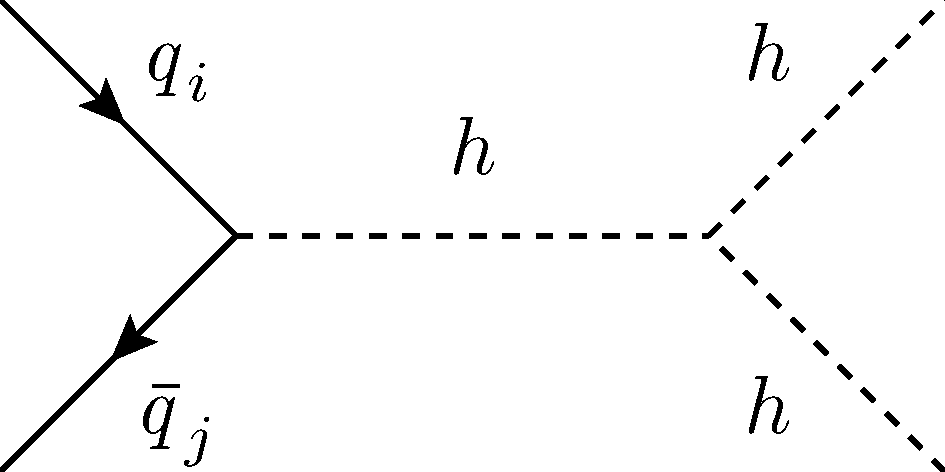
\includegraphics[scale =0.25]{./fig/qqh_higgs_prpg}}
		\put(20,120){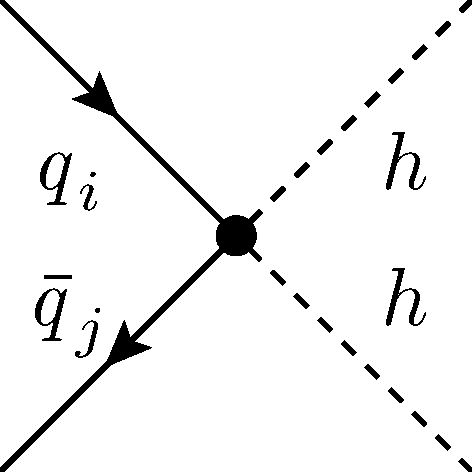
\includegraphics[scale = 0.25]{./fig/qqh_dim6}}
		\put(110,110){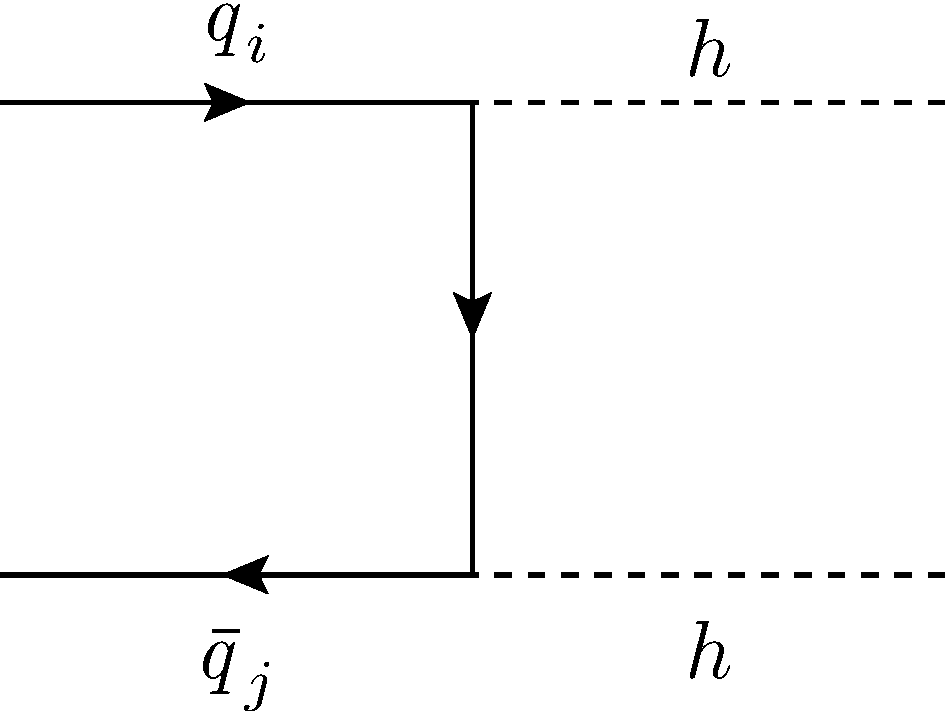
\includegraphics[scale =0.21]{./fig/qqh_tchannel}}
		\put(230,145 ){{\large+ crossed} }
	\end{picture}
	\vspace*{-4cm}
	\caption{ Feynman diagrams for the~$\qqA$ Higgs pair production in the SMEFT paradigm. The middle diagram shows a contact $hh q\bar q$ interaction that constructively interfere with the $s$-channel topology. Combined with the PDF enhancement,  Higgs pair production is significantly more sensitive to ligh Yukawa couplings compared to its single Higgs counterpart. }
	\label{qqA_fd}
\end{figure}
\begin{figure}[t]
	\centering
	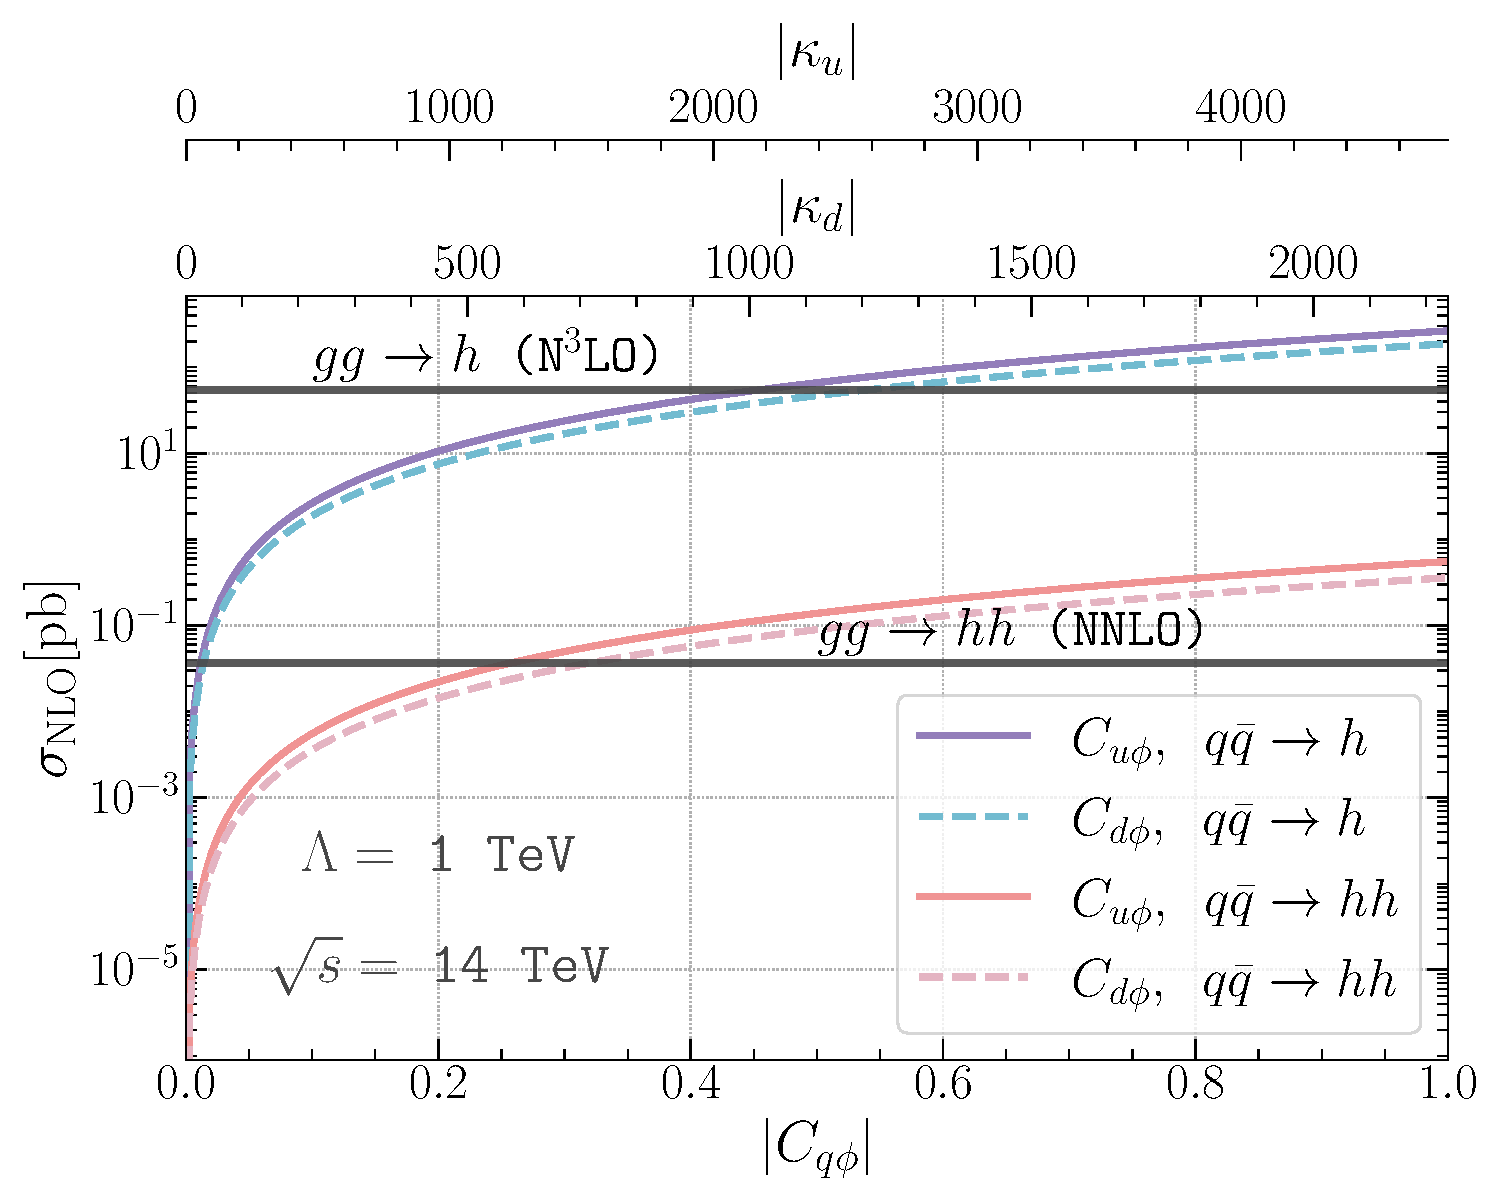
\includegraphics[width=0.75\textwidth]{fig/pph_hh_14Tev.pdf}
	\caption{ The production cross-section of single Higgs and di-Higgs at $14$ TeV from the quark anti-quark annihilation $q\bar{q}A$ as a function of the Wilson coefficients $C_{u\phi}$ and $C_{d\phi}$ versus the SM gluon fusion cross-sections, the horizontal solid line for gluon fusion channels. One can observe that for values of $C_{u\phi}=0.22\, (0.43)$ and $C_{d\phi}=0.26\, (0.47)$ the $q\bar{q}A$ channel becomes the dominant di-Higgs (single Higgs) production channel. The NP scale is set to $\Lambda = 1$ TeV. }
	\label{fig:pphhvsh}
\end{figure} 
\begin{figure}[!hb]
	\centering
	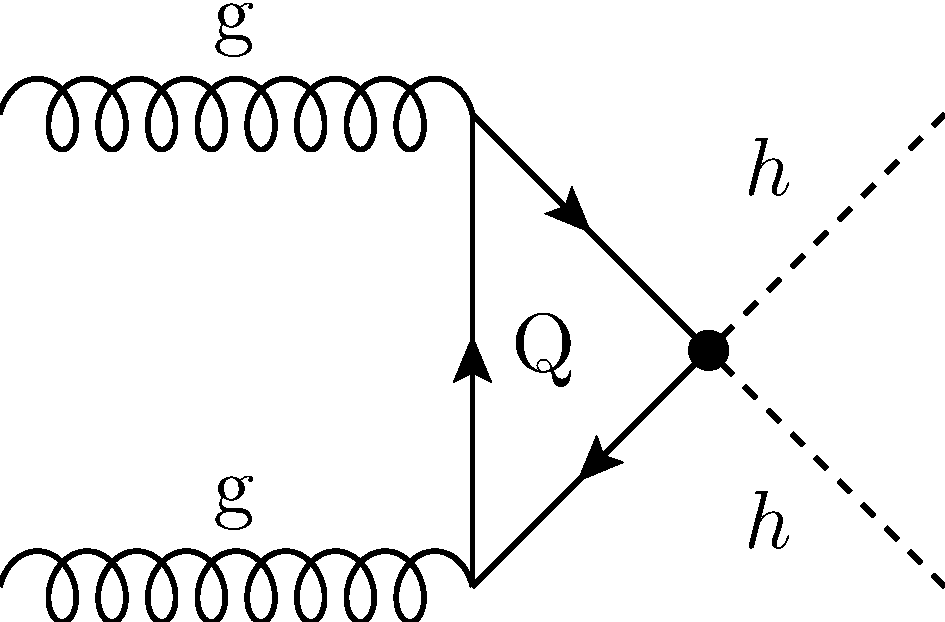
\includegraphics[width = 0.5\textwidth]{./fig/ggfdim6}
	\caption{The new diagram for ggF emerging from the~$hh q \bar q$ coupling appearing in SMEFT.}
	\label{fig_ggf_diag}
\end{figure}
This chapter aims to study the potential for Higgs pair production as a direct probe channel for light quark Yukawa interaction; focusing on the first generation quarks.  I will start by introducing the inclusion of light quark couplings to the Higgs in the SMEFT framework in~\autoref{sec:EFTlightyuk}. Then the NLO QCD calculation of the $\qqA$ channel is shown in~\autoref{sec:qqHH}. \autoref{sec:cutbasedly} outlines a cut-based analysis of the di-Higgs final state~$ b \bar b \gamma \gamma$ to estimate the sensitivity of this channel for the HL-LHC. Later, in~\autoref{sec:mlanalysisly} an optimised approach for enhancing the sensitivity based on multi-variant analysis and interpretable machine learning is showcased. The results of both analysis techniques are discussed and compared in ~\autoref{sec:resultsly} While in ~\autoref{sec:comparetoothers} I overview the other searches for light Yukawa couplings, comparing them to the Higgs pair production sensitivity. This chapter is concluded in~\autoref{sec:concly}. \\ The cut-based analysis has been published in~\cite{Alasfar:2019pmn}, while the interpretable machine-learning one is an undergoing project with R.~Gr\"ober, C.~Grojean, A.~Paul, and Z.~Qian, and expected to be published soon~\cite{IML}. 
%%%%%%%%%%%%%%%%%%%%%%%%%%%%%%%%%%%%%%%%%%%%%%%%%%
\section{SMEFT and light Yukawa couplings\label{sec:EFTlightyuk}}
%%%%%%%%%%%%%%%%%%%%%%%%%%%%%%%%%%%%%%%%%%%%%%%%%%
Explicitly writing the flavour indices~$ij$ of the SMEFT operators and lifting the condition of their flavour universality, we could get light quark -Higgs coupling enhancement from the operators
\begin{equation}
	\Delta \mathcal{L}_{y}=\frac{\phi^{\dagger}\phi}{\Lambda^2}\left( C_{u \phi}^{ij} \bar{Q}_L^i \tilde{\phi} u_R^j + C_{d \phi}^{ij} \bar{Q}_L^i \phi d_R^j +h.c.\right)\,,
	\label{eq:EFTop}
\end{equation}
The mass matrices of the up-and down-type quarks obtained from the Yukawa and the new SMEFT coupling are
%
\begin{align}
	M^u_{ij} =& \frac{v}{\sqrt{2}} \left( y^u_{ij}-\frac{1}{2} (C_{u\phi})_{ij}\frac{v^2}{\Lambda^2}\right)\,,\nonumber\\
	M^d_{ij} =& \frac{v}{\sqrt{2}} \left( y^d_{ij}-\frac{1}{2} (C_{d\phi})_{ij}\frac{v^2}{\Lambda^2}\right)\,, \label{eq:mass}
\end{align}
where $y^q_{ij}$ are the SM Yukawa matrix elements introduced in eq.~\eqref{lag-yuk}. Since the quark masses are measured quantities, one would naturally rotate to the mass basis using bi-unitary transformation represented by the matrices~$ \mathcal{V}_q, \mathcal{U}_q$, like in the SM. The Wilson coefficients matrix elements in the flavour space in the mass basis can be written as
\begin{equation}
	\tilde{C}_{q \phi}^{ij}= \left(\mathcal{V}_{q}\right)^*_{ni}C^{nm}_{q\phi}\left( \mathcal U_{q}\right)_{mj}\, , \; \; \; \;  \text{with } \;\;\;\;\; q = u,d\, .
\end{equation}
In order to match these Wilson coefficients to Higgs couplings to quarks,  the Lagrangian operator describing these couplings is used
\begin{equation}
	\mathcal{L}\supset g_{h\bar{q}_i q_j}\bar{q}_i q_j h + g_{h\bar{q}_i q_j}\bar{q}_i q_j h^2
\end{equation}
Then, one gets the matching results in identifying the SMEFT couplings of Higgs and quarks
\begin{equation}
	g_{h\bar{q}_i q_j} := \quad \frac{m_{q_i}}{v}\delta_{ij}-\frac{v^2}{\Lambda^2} \frac{	\tilde{C}_{q \phi}^{ij}}{\sqrt{2}}\,, \quad \quad \quad \quad \quad g_{h h\bar{q}_i q_j} := \quad -\frac{3}{2\sqrt{2}}\frac{v}{\Lambda^2}	\tilde{C}_{q \phi}^{ij}\,. \label{eq:couplingsEFT}
\end{equation}
It is possible to observe that, in the general case,  non-diagonal couplings can be generated. However, such couplings are strongly constraint by flavour observables, particularly neutral meson mixing~\cite{Blankenburg:2012ex}.
\begin{equation}
	|\tilde{C}_{q\phi}^{12}| \lesssim 10^{-5} \Lambda^2/v^2| \quad \quad  \quad \quad | \tilde{C}_{d\phi}^{13/23}| \lesssim 10^{-4} \Lambda^2/v^2.
\end{equation}
Due to these strong constraints, it is typical to consider SMEFT with minimal flavour violation~(MFV)~\cite{DAmbrosio:2002vsn}, in which the SM Yukawa matrices~$y_q^{ij}$ are the only spurions breaking the global~$SU(3)_Q \otimes SU(3)_U \otimes SU(3)_D \to U^6(1)$ flavour symmetry. This implies that the Wilson coefficients matrices in the mass basis are simultaneously diagonalisable with the SM Yukawa matrices and inherit their hierarchy.  Therefore,  MFV is not a viable scheme for considering significant enhancements to the couplings for first and second generations while keeping the third generation couplings unchanged. \\ In order to bypass the constraints of MFV and also avoid flavour changing neutral currents~(FCNC) that are prohibited by flavour observables, one needs to turn to flavour alignment~\cite{Pich:2009sp,Pich:2010ic} or its generalisation aligned flavour violation~(AFV)~\cite{Egana-Ugrinovic:2018znw}. \\ 
With flavour alignment schemes, the NP flavour parameters~(here the Wilson coefficients) are aligned with the SM Yukawa, such that both can be simultaneously diagonalised, thus preventing tree-level FCNCs.  Contrary to MFV, the duress of making these new parameters proportional to the SM Yukawa couplings is lifted. This would induce radiative FCNCs, as this formalism in unstable under quantum corrections ~\cite{Ferreira:2010xe,Jung:2010ik,Botella:2015yfa}. This alignment breaking would not be seen in the SMEFT but rather when UV-complete models are considered. AFV resolves this instability by ensuring that any NP Spurion breaking the flavour symmetry will transform trivially under the quark phases transformations $ U^6(1)$, keeping the CKM matrix the only flavour object that has non-trivial transformations. Thereby the CKM will have physical flavour changing currents as well as a $\mathcal{CP}$-violating phase. This constraint on the NP flavour spurions $k_q$, allows them to be written as a series in powers of the CKM matrix, known as the alignment expansion
\begin{align}
	k_u &= K_{0,u}+ K_{1,u} V^*_{CKM} K_{2,u} V^T_{CKM} K_{3,u} + \mathcal O(V^4_{CKM})+ \dots,  \\
	(k_d)^\dagger&=K_{0,d}+ K_{1,d} V^T_{CKM} K_{2,d} V^*_{CKM} K_{3,d} + \mathcal O(V^4_{CKM}) + \dots,
	\label{eqK}
\end{align}
where $K_{i,u}$ and $K_{i,d}$ are complex $3\times3$ diagonal matrices invariant under flavour transformations. This formalism is stable under renormalisation group evolution as any linear combinations, or tensor products of the spurions will remain flavour aligned. \\
For simplicity, I shall only consider the first term in the alignment expansion, such that only diagonal $C_{q\phi}$ are investigated, as the other terms are already CKM-suppressed and not of particular phenomenological interest.  With this in mind, and using the translation between SMEFT and $\kappa$-formalism discussed in~\autoref{eftkappa}, it is possible to identify the couplings in SMEFT with the $\kappa$'s
\begin{equation}
	g_{h\bar{q}_i q_i} =\kappa_q g_{h\bar{q}_i q_i}^{\text{SM}} \,, \quad \quad \quad \quad \quad g_{h h\bar{q}_i q_i}= - \frac{3}{2}\frac{1-\kappa_q}{v}g_{h\bar{q}_i q_i}^{\text{SM}} \,,
	\label{eq:def_kappa}
\end{equation}
in a slight abuse of language of the $\kappa$-formalism as the $hhq \bar q$ coupling typically is not included in it.
\par
Higgs pair production offers an extra advantage for probing light Yukawa interactions, as it is susceptible to the $hh q\bar q$ interaction; one could also consider the non-linear HEFT by extending it to include Wilson coefficients $c_q$ and $c_{qq}$ for the first and second-generation quarks, in analogy to ones defined for the top quark in eq.~\eqref{eq:coupl_def}~ \cite{Contino:2010mh}. The analysis performed on these HEFT parameters is published in~\cite{Alasfar:2019pmn}. 
%%%%%%%%%%%%%%%%%%%%%%%%%%%%%%%%%%%%%%%%%%%%%%%%%%
\section{Higgs pair production and Higgs decays with modified light Yukawa couplings \label{sec:qqHH}}
%%%%%%%%%%%%%%%%%%%%%%%%%%%%%%%%%%%%%%%%%%%%%%%
As we have briefly discussed in the introduction, the gluon fusion channel of Higgs pair production is affected by enhanced light Yukawa couplings in two ways: First is the inclusion of light quark loops in the triangle and box diagrams. Second, the new diagrams introduced by the contact $hh q\bar q$ coupling are shown in~\autoref{fig_ggf_diag}. However, these effects are negligible due to the mass-suppression of these diagrams by the light quark appearing in the loops. Therefore, effectively, one could consider the ggF channel as purely derived by third-generation quarks and only affected by the trilinear coupling~$C_\phi$ as far as this analysis is concerned.
%This benchmark is inspired by ref.~\cite{Bar-Shalom:2018rjs}.
\subsection{Higgs pair production via quark anti-quark annihilation}
Contrary to the ggF, the $\qqA$ channel is severely suppressed by quark masses in the SM.  In fact, if  these quarks are considered massless, like in the 5-flavour scheme, this channel vanishes in the SM.  There are four-diagrams contributing to $\qqA$ shown in~\autoref{qqA_fd}, computing the matrix-elements for it gives the differential partonic cross-section 
\begin{align}
	\frac{d \hat \sigma_{q_i\bar{q}_j}}{d \hat t} &= \frac{1}{16 \pi}\, \frac{1}{12  \hat{s}} \bigg[ \left| 2  g_{hh q_i \bar q_j} + \frac{g_{hhh}\, g_{h q_i \bar q_j}}{\hat{s}-m_h^2-im_h\Gamma_h}\right|^2+ \mathcal{O}(g_{h q_i \bar q_j}^4) \bigg],
	\label{sigmaqqa}
\end{align}
where the~$ \mathcal{O}(g_{h q_i \bar q_j}^4)$ terms stem from the $\hat{t}$- and $\hat{u}$-channel diagrams, and their contribution is typically only $\sim 0.1 \%$ of the total cross-section.
The hadronic cross section is then obtained by
\begin{equation}
	\sigma_{\mathrm{hadronic}} =  \int_{\tau_0}^1 d\tau \int_{\hat{t}_-}^{\hat{t}_+} d\hat{t} \sum_{i,j} \frac{d\mathcal{L}^{q_i\bar{q}_j}}{d\tau}\frac{ d\hat \sigma_{q_i\bar{q}_j}}{d \hat t}\,, \label{eq:sigmahadron}
\end{equation}
with $ \tau_0= 4\, m_h^2/s$, $\hat{s}=\tau s$ and
\begin{equation}
	\hat{t}_{\pm}=m_h^2-\frac{\hat{s}(1\mp \beta)}{2} \quad\quad \text{and}\quad \quad \beta=\sqrt{1-\frac{4 m_h^2}{\hat{s}}}\,.
\end{equation}
The parton luminosity is given by
\begin{equation}
	\frac{d{\cal L}^{q_i \bar q_j}}{d\tau} = \int_\tau ^1 \frac{dx}{x} \,\left[  f_{q_i}(x/\tau,\mu_F^2) f_{\bar{q}_j}(x,\mu_F^2) + \,f_{\bar{q}_j}(x/\tau,\mu_F^2) f_{q_i}(x,\mu_F^2)\right]\,.
\end{equation}
All the kinematic masses were neglected, following the 5-flavour scheme of the PDFa, while the coupling of the Higgs boson to the light quarks (for flavour diagonal couplings) is
\begin{equation}
	g_{hq_i\bar{q}_j}=\frac{m^{\bar{MS}}_q(\mu_R)}{v}  \kappa_q \delta_{ij}\,,
\end{equation}
and analogously for the $g_{hhq_i\bar{q}_j}$ coupling.  It is worth noting that there is no inconsistency with such an assumption since, in scenarios of modified Yukawa couplings, the masses of the quarks need not be generated by electroweak symmetry breaking.
%%%%%%%%%%%%%%%%%%%%%%%%%%%%%%%%
\subsubsection{NLO QCD correction \label{sec:qqA_NLO}}
%%%%%%%%%%%%%%%%%%%%%%%%%%%%%%%%
Since the ggF NLO QCD corrections are sizeable,  it is reasonable to assume that the same would apply to the $\qqA$ similitude.  Computing the NLO QCD corrections to this channel is a relatively straightforward task. More simplifications can be made by neglecting the NLO corrections of the $\hat{t}$ and $\hat{u}$ channels because they are strongly suppressed.  This enables us to adapt the NLO QCD corrections results from $ b \bar b \to h$ in the 5-flavour scheme~\cite{Dicus:1998hs, Balazs:1998sb, Harlander:2003ai}, also for $b\bar{b}hh$~\cite{Dawson:2006dm, H:2018hqz}, to the $s$-channel and contract term $\qqA$ diagrams. This is achieved by some adjustments taking into account the modified LO cross-section and the different kinematics of the process.
The Feynman diagrams at NLO QCD are shown in~\autoref{qqA_nlo}.
%%
\begin{figure}[!t]
	\centering
	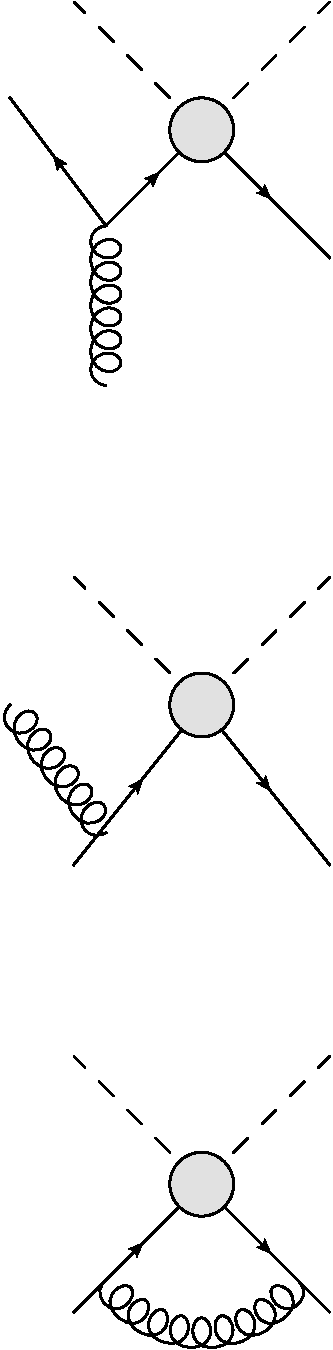
\includegraphics[width = 0.20\textwidth, angle = -90]{./fig/qqbar_hh_nlo.pdf}
	\caption{Generic form of the QCD corrections of order~$\mathcal O(\alpha_s)$ to the $\qqA$ Higgs pair production. }
	\label{qqA_nlo}
\end{figure}
%%
The NLO corrections are given by~\cite{Spira:2016ztx}
%%
\begin{subequations}
	\begin{eqnarray}
		\sigma(q\bar q\to h) & = & \sigma_{LO} + \Delta\sigma_{q\bar q} +
		\Delta\sigma_{qg},  \\
		\Delta\sigma_{q\bar q} & = & \frac{\alpha_s(\mu_R)}{\pi} \int_{\tau_0}^1
		d\tau \sum_q \frac{d{\cal L}^{q\bar q}}{d\tau} ~\int_\tau^1 dz~\hat{\sigma}_{LO}(Q^2=z\tau s)~\omega_{q\bar
			q}(z) , \\
		\Delta\sigma_{qg} & = & \frac{\alpha_s(\mu_R)}{\pi} \int_{\tau_0}^1 d\tau
		\sum_{q,\bar q} \frac{d{\cal L}^{qg}}{d\tau}~\int_\tau^1 dz~\hat{\sigma}_{LO}(Q^2=z\tau s)~\omega_{qg}(z),
	\end{eqnarray}
\end{subequations}
and
\begin{equation}
	\hat{\sigma}_{LO}(Q^2)= \int_{\hat{t}_-}^{\hat{t}_+} \frac{ d\hat \sigma_{q_i\bar{q}_j}}{d \hat t},
\end{equation}
%%
with $z=\tau_0/\tau$, $\sigma_{LO}=\sigma_{\mathrm{hadronic}}$ of eq.~\eqref{eq:sigmahadron}, and the $\omega$ factors are given by \\
%%
\begin{subequations}
	\begin{eqnarray}
		\omega_{q\bar q}(z) & = & -P_{qq}(z) \ln \frac{\mu_F^2}{\tau s}
		+ \frac{4}{3}\left\{ \left(2\zeta_2-1 +
		\frac{3}{2}\ln\frac{\mu_R^2}{M_{hh}^2} \right)\delta(1-z)  \right. \\ &+ & \left.  (1+z^2) \left[
		2 {\cal D}_1(z) - \frac{\ln z}{1-z} \right] + 1-z \right\} \nonumber \,, \\
		\omega_{qg}(z) & = & -\frac{1}{2} P_{qg}(z) \ln \left(
		\frac{\mu_F^2}{(1-z)^2 \tau s} \right) - \frac{1}{8}(1-z)(3-7z)\,,
	\end{eqnarray}
\end{subequations}
%%
with $ \zeta_2 = \frac{\pi^2}{6}$.
The Altarelli Parisi splitting functions $ P_{qq}(z)$ and $ P_{qg}(z)$~\cite{gribov1972deep,Altarelli:1977zs,Dokshitzer:1977sg} are given by
\begin{subequations}
	\begin{align}
		P_{qq}(z) & = \frac{4}{3} \, \left[2{\cal D}_0(z)-1-z+\frac{3}{2}\, \delta(1-z)\right],  \\
		P_{qg} &= \frac{1}{2}\, \left[  z^2+(1-z)^2\right],
	\end{align}
\end{subequations}
and the ``plus'' distribution is
\begin{equation}
	{\cal D}_n(z) := \left(\frac{\ln(1-z)^n}{1-z} \right)_+.
\end{equation}
The renormalisation scale $ \mu_R = M_{hh}$ and the factorisation scale $ \mu_F= M_{hh}/4$, were chosen as central values. \\
The NLO $\qqA$ cross-section as well as the LO ggF were implemented in a private FORTRAN code utilising the \texttt{VEGAS} integration algorithm, and NNPDF30 parton distribution functions~(PDF's)\cite{Ball:2017nwa} available through the \texttt{LHAPDF-6} package \cite{Buckley:2014ana}. For the one-loop integrals appearing in the form-factors of the box and triangle diagrams, I have used the \textsc{Collier} library~\cite{Denner:2014gla} to ensure numerical stability of the loop integral calculation for massless quarks inside the loops~\footnote{I have expanded the code to include other SMEFT operators, and it can be found in the \texttt{GitHub} repository \url{https://github.com/alasfar-lina/HH_XS_in_SMEFT} }. 
The resulting NLO $K$-factor was found to be
\begin{equation}
	K_{NLO}=\frac{\sigma_{NLO}}{\sigma_{LO}} = 1.28 \pm 0.02\,,
\end{equation}
with the error denoting the theoretical uncertainty.
The $K$-factor does not depend on the scaling of the couplings nor the flavour of the initial $q \bar q$ since the LO cross-section factors out (except for the different integration in the real contributions). \\
%The $\qqA$ channel enhance the overall Higgs pair production cross-section. Still, if one considers the ggF as an SM background for the Yukawa enhancement  ``signal'' $\qqA$ channel, it would be interesting to estimate qualitatively when this signal becomes dominant, further emphasising the sensitivity of Higgs pair to light Yukawa enhancements as~\autoref{fig:pphhvsh} demonstrates.
%The dominant term for  $\qqA$ comes from the $hh q \bar q$ vertex diagram, such that the $\qqA$ cross-section behaves for large values of $\kappa$ as (assuming that $ \sigma^{qqA}_{SM}\sim 0 $)
%\begin{equation}
%	(\sigma^{qqA}-\sigma^{qqA}_{SM}) \sim  g_{hh q \bar q}^2 \sim v^{-4}\,{m_q^2\,\kappa_q^2}.
%\end{equation}
%The ggF cross-section instead gets contributions from light quark loops interfering with top quark loops in the triangle SM diagram,  leading to scaling of
%\begin{equation}
%	(\sigma^{ggF} - \sigma^{ggF}_{SM} ) \sim  \kappa_q\, \frac{m_q^2}{ v^2\,M_{hh}^2}\,\ln^2{\left(\frac{M_{hh}}{m_q}\right)}\,.
%\end{equation}
%Taking the ratio we get
%\begin{equation}
%	\frac{(\sigma^{qqA}-\sigma^{qqA}_{SM})}{(\sigma^{ggF} - \sigma^{ggF}_{SM} )} \sim  \frac{\kappa_q}{ v^2\left(\frac{
%			\ln^2{\left(\frac{M_{hh}}{m_q}\right)}}{M_{hh}^2}\right)}\,.
%\end{equation}
%This ratio approaches one (neglecting effects from different PDFs) when
%\begin{equation}
%	\kappa_q^{qqA = ggF} \sim  \frac{v^2\,\ln^2{\left(\frac{M_{hh}}{m_q}\right)}}{M_{hh}^2}\,.
%\end{equation}
%Using this order of magnitude estimate, we see that  the two cross sections are roughly equal if $\kappa_c^{qqA = ggF} \sim 1$, $\kappa_s^{qqA = ggF} \sim 10$ and $\kappa_u^{qqA = ggF} \sim \kappa_d^{qqA = ggF} \sim 10^3$.
%The actual values of $\kappa_q^{qqA = ggF}$ for the first generation quarks can be read from fig.~\ref{pphhvsh}.It is interesting to point out to the pact that these $\kappa_q$ values are not yet excluded.
%%%%%%%%%%%%%%%%%%%%%%%%%%%%%%%
\subsection{Higgs decays \label{sec:Hdecay}}
%%%%%%%%%%%%%%%%%%%%%%%%%%%%%%%
The same way $hh$ production acquires additional channels due to enhanced Yukawa couplings, also Higgs decays to light quarks will become significant compared to the SM scenario~\cite{deFlorian:2016spz}.  In addition to the contribution of light quarks in the loop-level decays~$h \to \gamma \gamma/Z \gamma$ and $ h \to gg$, though this effect is small.  Since the $ h \to q\bar q$ decay are near impossible to detect with the current technologies, the effect of opening these decay channels is reduction in the branching ratios of the Higgs final states of experimental interest, like $ h \to b \bar b $ and $ h \to \gamma \gamma$. \\ In order to compute the Higgs partial widths and branching ratios (BR) at higher orders in QCD, I have modified the FORTRAN programme \texttt{HDECAY}~\cite{Djouadi:1997yw,Djouadi:2018xqq} to include the light fermion decay channels and loops in the above-mentioned decays~\footnote{The modified \texttt{HDECAY} code can be found in the \texttt{GitHub} repository \url{https://github.com/alasfar-lina/hdecay_lightflavour}}. The overall change of the Higgs total width is given by
\begin{equation}
	\Gamma_H \approx \Gamma_{\text{SM}}+\sum_{q=c,s,u,d}\frac{g_{h \bar{q}_i q_i}^2}{(g_{h \bar{q}_i q_i}^{\text{SM}})^2}\Gamma_{q}\,,
\end{equation}
where $\Gamma_q$ can be obtained at NLO QCD from the modified ~\texttt{HDECAY} code. Detailed results for the Branching ratios for the final states of interest have been published in~\cite{Alasfar:2019pmn}.\\ 
%###
In order to have a preliminary estimate about the sensitivity of Higgs pair production to light Yukawa enhancements, it is important to consider both production and decay effects in terms of signal strength
\begin{equation}
	\mu_i : = \frac{\sigma \, {\rm BR}_i } {\sigma^{\SM} \, {\rm BR}_i^{\SM}}.
\end{equation}
Comparing the production of single Higgs to Higgs pair signal strengths, for any final state of interest, we could see in~\autoref{signal_strength_hh} that for first-generation $C_{q \phi} \lsim 0.8$ Higgs pair production has a higher signal strength than single-Higgs production despite having double the reduction in the signal strength from the decays of two Higgs bosons as opposed to a single one. 
\begin{figure}[!t]
	\centering
	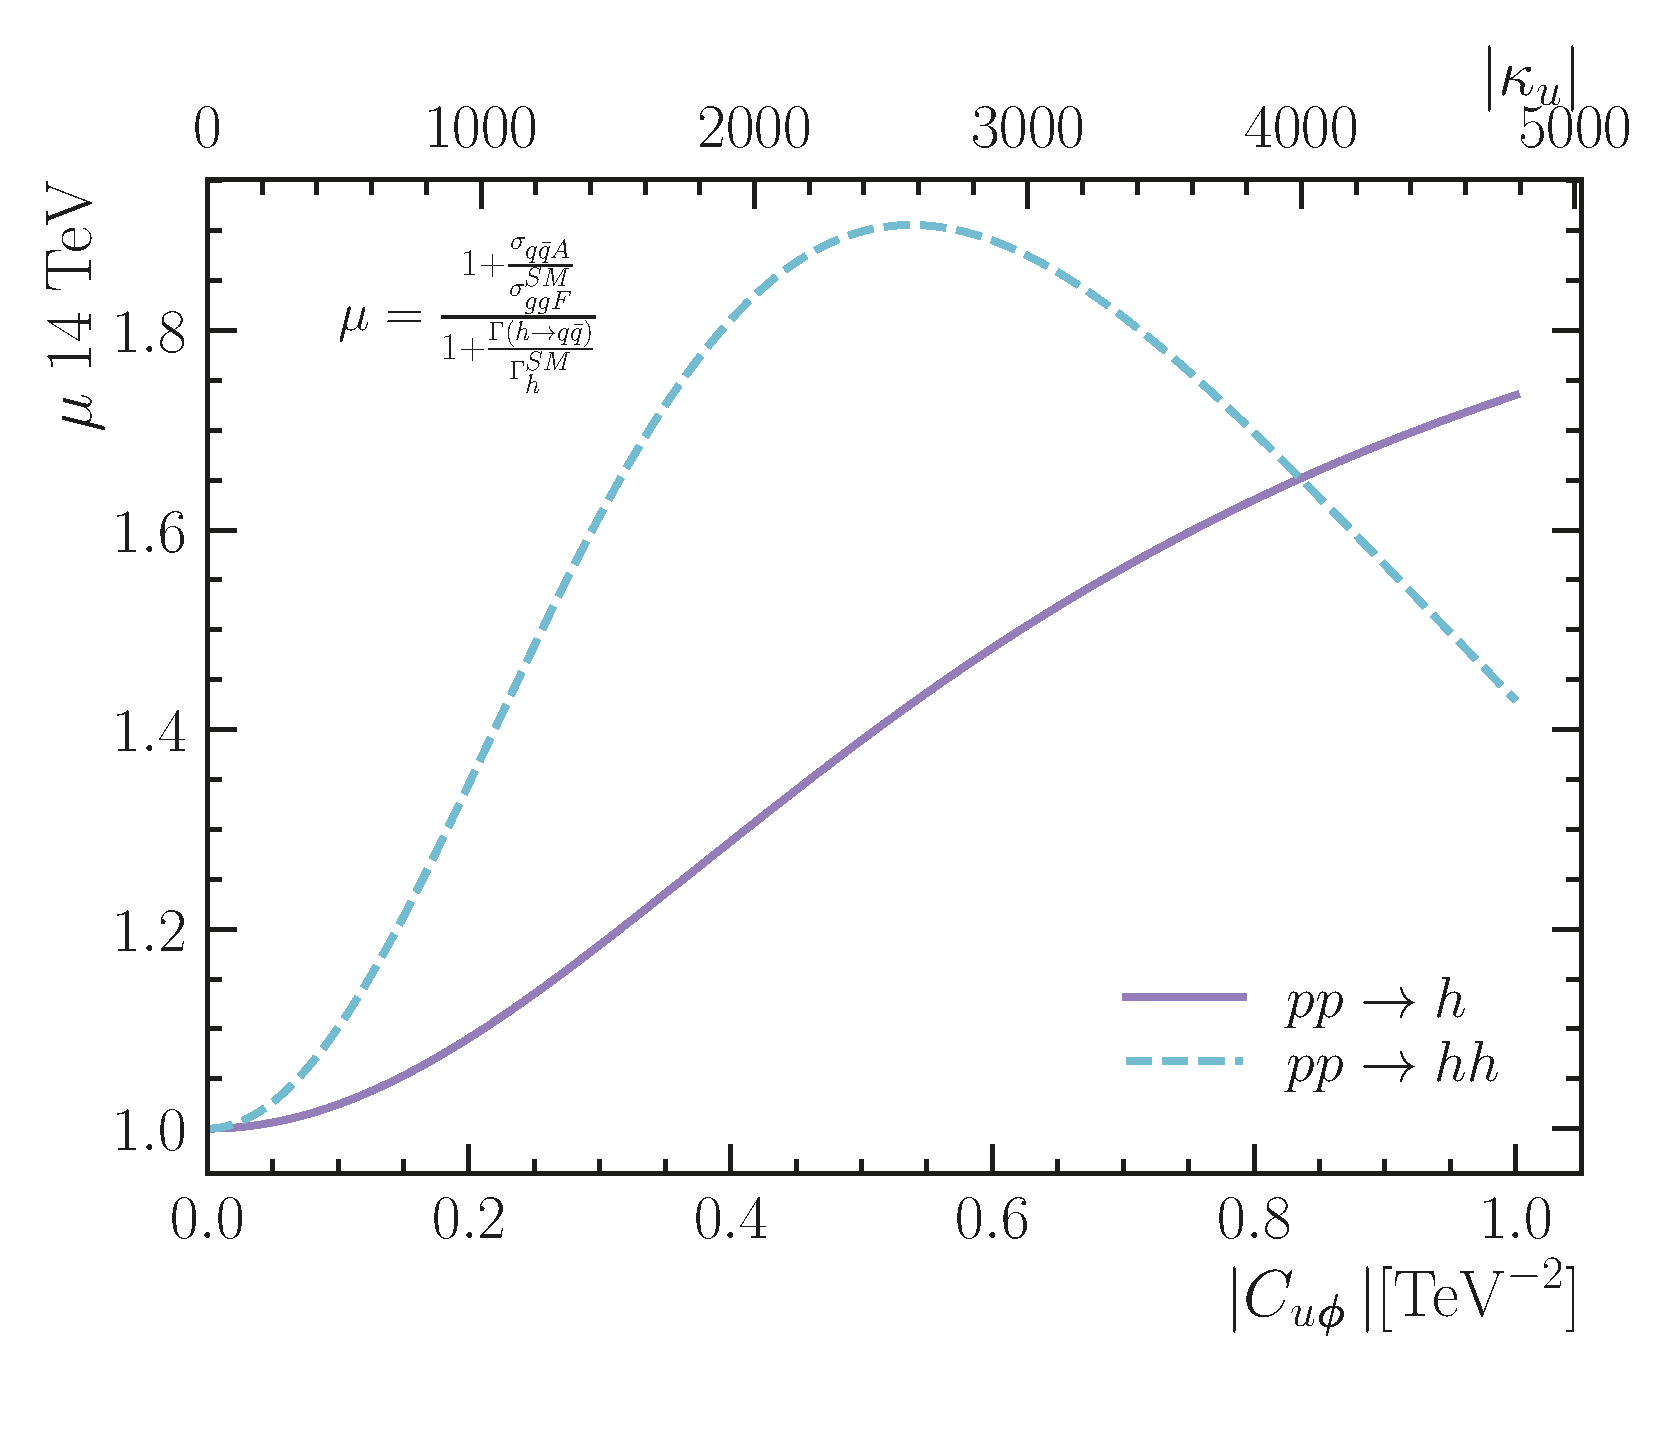
\includegraphics[width = 0.49\textwidth]{./figures/up-signal-strength.pdf}
	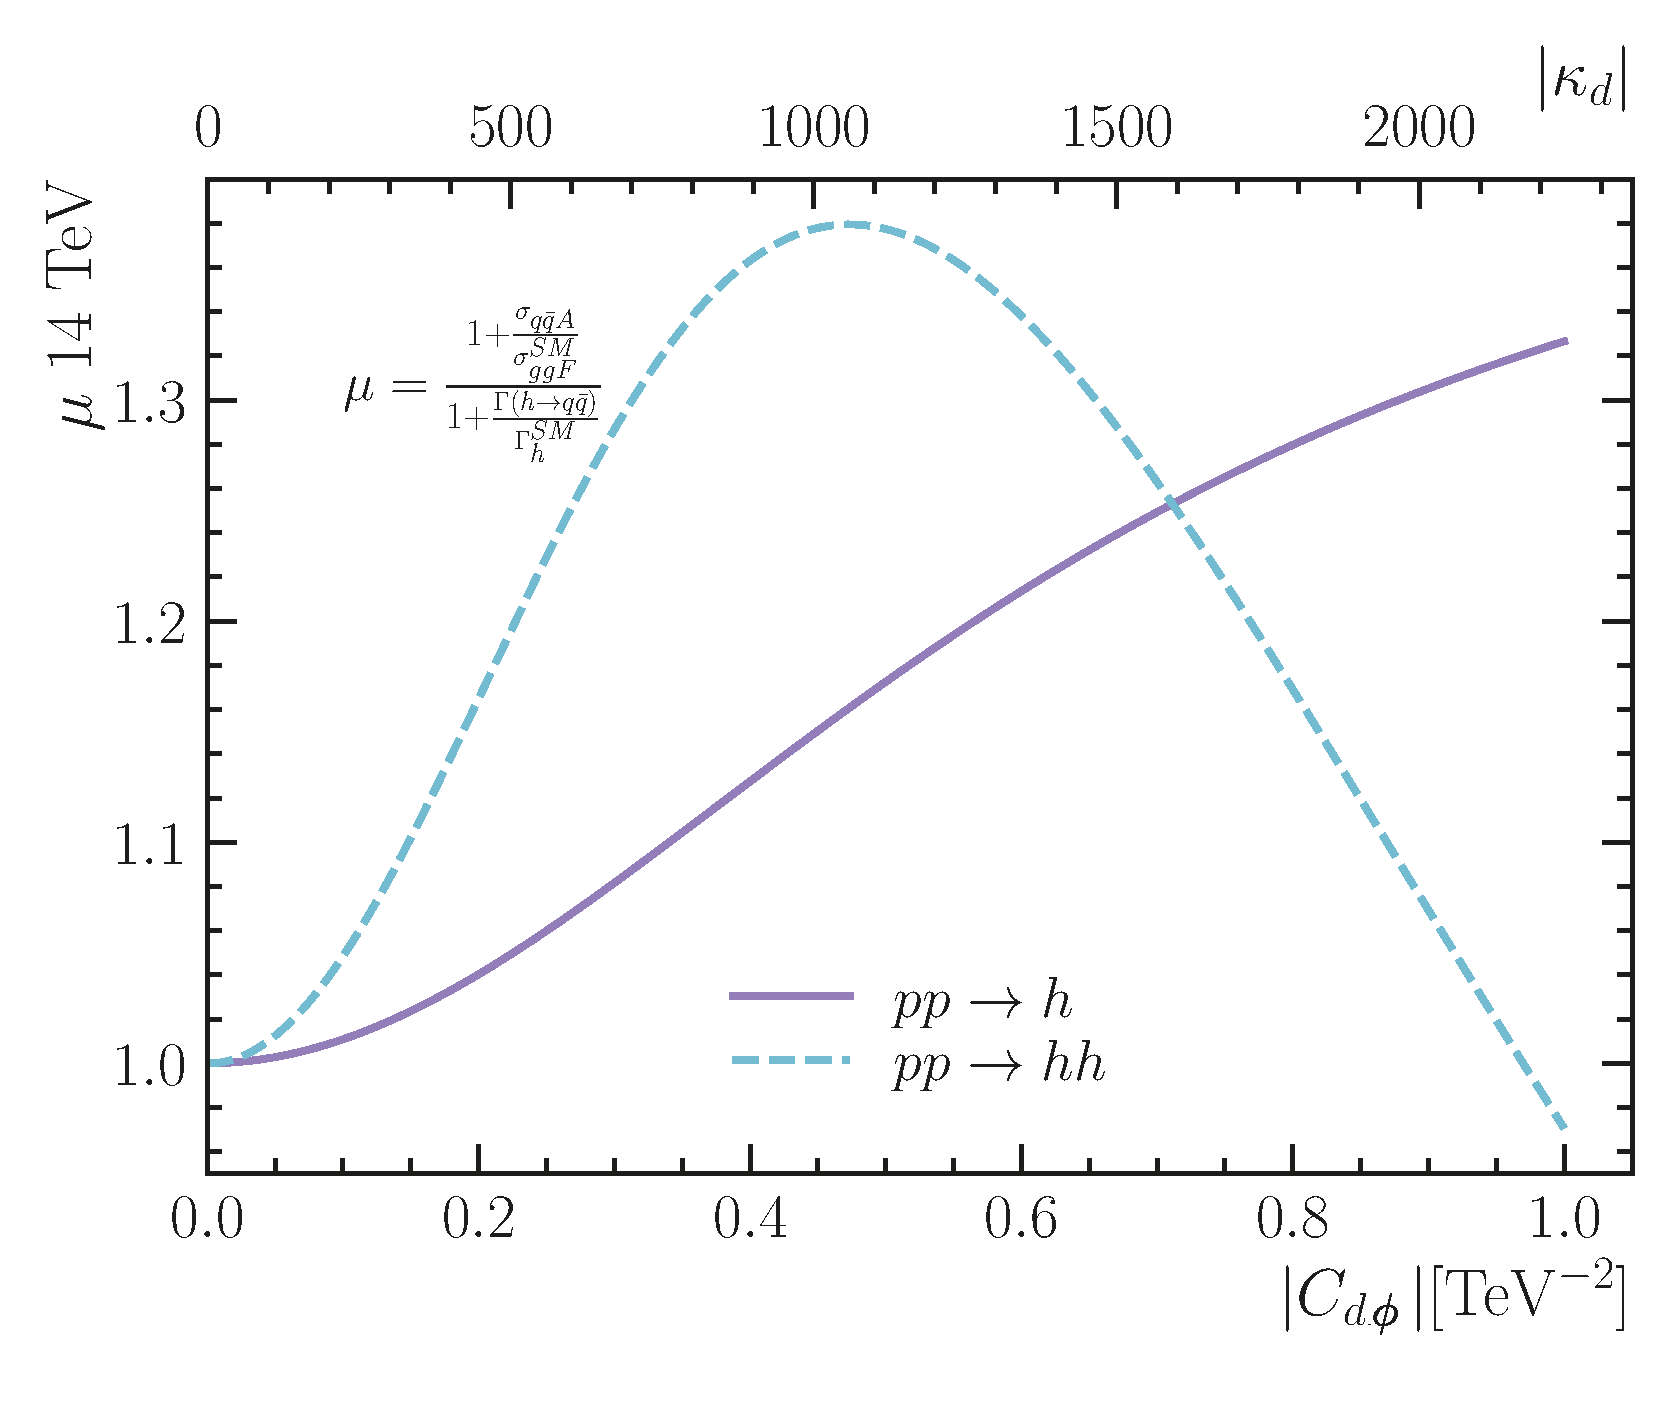
\includegraphics[width = 0.49\textwidth]{./figures/dn-signal-strength}
	\caption{Signal strengths at 14 TeV LHC, of the single Higgs (purple solid line) vs. Higgs pair (blue dashed line) as functions of $C_{u\phi}$ (left) and $C_{d \phi}$ (right). Both plots show that for $C_{q \phi} \lsim 0.8$  the signal strength of Higgs pair production is higher than the single Higgs one. This implies that Higgs pair production is more sensitive to enhancements of light quark Yukawa in SMEFT. This is independent of the final state (except for $ h \to q \bar q$).  }
	\label{signal_strength_hh}
\end{figure}
In fact, and as we shall see in~\autoref{sec:comparetoothers}, values of $C_{q \phi} >0.4$ have been already excluded by multiple searches. 
%%%%%%%%%%%%%%%%%%%%%%%%%%%%%%%
\section{Event generation for the final state $ hh \to b \bar b \gamma \gamma$ \label{sec:evnt}}
%%%%%%%%%%%%%%%%%%%%%%%%%%%%%%%
For this study, the final state~$b \bar{b} \gamma \gamma$ is considered, as this channel has the most potential for Higgs pair searches~\cite{Cepeda:2019klc}. It has the ``clean'' $h \to \gamma \gamma$ decay, but also the other Higgs decay to $b$-quark pair is a channel with a large branching ratio~$\sim 58\%$ and b-tagging capabilities for ATLAS and CMS are continuously improving. \\
\par 
For the cut-based analysis, the FORTRAN codes used to compute the $hh$ cross-section and decay have been interfaced with ~\texttt{Pythia} 6.4~\cite{Sjostrand:2006za}, where the $\qqA$ process was generated at NLO and the ggF at LO, then multiplied with the NLO K-factor. The generated events were written to a ROOT file via \texttt{RootTuple} tool~\cite{roottuple} for further analysis. \\ The backgrounds were not simulated for this analysis; rather, the results from ~\cite{Azatov:2015oxa} were used because we have used the same cuts as this reference.
\par 
For the multivariate analysis based on interpretable BDT, the backgrounds and signal events needed to be generated. The backgrounds described in~\autoref{tab:xsec14} were generated using~\texttt{MadGraph\_aMC@NLO}~\cite{Alwall:2014hca}, then showered via ~\texttt{Pythia 8.3}~\cite{Sjostrand:2014zea} and a fast detector simulation is done using \texttt{Delphes 3}~\cite{deFavereau:2013fsa}, the QED/QCD background $ b \bar b\gamma \gamma$, $Zh$  and $ b \bar b h$ events were taken from the analysis data of ref.~\cite{Grojean:2020ech}, while $t \bar t h $ events were generated specifically for this analysis. In order to obtain the NLO cross-section for these process, the events were multiplied by their respective $K$-factors that have been obtained from~$t\bar{t}h$~\cite{Beenakker:2001rj}, $b\bar b \gamma\gamma$~\cite{Fah:2017wlf}, $Zh$~\cite{Campanario:2014lza} and the remaining part of the $b\bar bh$ processes from~\cite{Dawson:2005vi}. \\ 
The Higgs pair signals were generated in a slightly different pipeline. The ggF channel events were simulated first using \texttt{POWHEG}~\cite{Heinrich:2017kxx,Heinrich:2019bkc,Heinrich:2020ckp}, which has been modified to separate the individual contributions from the box, triangle, and their interference.  This is done to easily scale by $\kappa_\lambda$ (or $C_\phi$), as the box does not depend on it, while the triangle and the interference have quadratic and linear dependence, respectively. The $\qqA$ channel events were generated via~\texttt{MadGraph\_aMC@NLO} using a model created with \texttt{FeynRules}~\cite{Alloul:2013bka}. Samples for both up-and down-quark initiated $q\bar q$A processes have been generated. Parton showering and fast detector simulation for both Higgs pair processes were run through the same pipeline as the backgrounds. This also goes for the scaling by the NLO  of $ \qqA$ and NNLO for ggF $K$-factors after the event generation. The Higgs bosons were decayed with the assumption of narrow width approximation, and the BR values were computed in the modified \texttt{HDECAY} code. 
\\
To be inclusive and to explore the capabilities and importance of the full detector coverage, no generator-level cuts were applied on these processes except for the $b\bar b \gamma\gamma$  to avoid divergences. These minimal generator-level cuts for $b\bar b\gamma\gamma$ are
\begin{equation}
	\begin{aligned}
		& Xp_T^b>20\,\gev, \\
		\textrm{generator level cuts:}\qquad& \eta_\gamma<4.2,~ \Delta R_{b\gamma}>0.2, \\
		& 100< m_{\gamma\gamma} \,(\gev) < 150.
	\end{aligned}
\end{equation}
Here $Xp_T^b$ implies a minimum $p_T$ cut for at least one $b$-jet. 
After the showering and detector simulation, further basic selection cuts were applied to select events with
\begin{equation}
	\textrm{basic cuts:}\qquad
	\begin{array}{l}
		n_{\mathrm{eff}}^{bjet}\geq 1,~n_{eff}^{\gamma jet} \geq 2,\\
		p_T^{bjet}>30\,\gev,~p_T^{\gamma jet}>5\,\gev,\\
		\eta_{bjet,\gamma jet}<4,~ 110\, \gev < m_{\gamma_1\gamma_2} < 140\,\gev,
	\end{array}
	\label{eqn:bcuts}
\end{equation}
and $n_{eff}^{b/\gamma jet}$ representing the number of $b/\gamma$-jets that pass the basic selection. The cross-section, $K$-factors, number of events with 6ab$^{-1}$ luminosity at 14 TeV are given in~\autoref{tab:xsec14} for the background and in~ \autoref{tab:kfact} for the Higgs pair signals. 
\begin{table}[t]
	\centering
	\begin{tabular}{ccccc}
		\toprule
		Channel	        &LO $\sigma $ [fb]	&$K$-fact.	&Order&6$\inab$ [\#evt @ order]   \\
		\midrule
		$\hhtri$	        &  $7.288 \cdot10^{-3}$    & 2.28 &\multirow{3}{*}{NNLO}   &  96   \\ 
		$\hhbox$            & $0.054$    & 1.98 &  & 680   \\ 
		$\hhint$            &$-0.036$    & 2.15 &  &-460   \\ 
		$\uuA$ $(C_{d\phi}=0.1)$ &  $2.753$    & 1.29&\multirow{2}{*}{NLO} &  28   \\ 
		$\ddA$ $(C_{u\phi}=0.1)$ &  $4.270$    & 1.30 & &  43   \\ 
		\bottomrule
	\end{tabular}
	\caption{  The LO cross-section for Higgs pair production processes~(including the decay $hh \to b \bar b \gamma \gamma$ ) for 6$\inab$ 14 TeV HL-LHC.}
	\label{tab:kfact}
\end{table}
Both analysis methods included sensitivity studies for the HL-LHC, i.e. 14 TeV and 6$\inab$~\footnote{In the published cut-based analysis~\cite{Alasfar:2019pmn} 3$\inab$ luminosity for the HL-LHC were used. However, here I used 6$\inab$ when reporting fit results} luminosity and projections for a future hadron circular collider (FCC-hh), with 100 TeV and the luminosity of 30 ab$^{-1}$ have been made for the ML-based analysis. The results for the FCC can be found in the~\autoref{app:fcc}.

%%%%%%%%%%%%%%%%%%%%%%%%%%%%%%%
\section{Cut-based analysis \label{sec:cutbasedly}}
%%%%%%%%%%%%%%%%%%%%%%%%%%%%%%%
A cut and count analysis has been performed mainly as a ``proof of concept'' to demonstrate the sensitivity of Higgs pair production for probing light quark Yukawa couplings.  The analysis used the same cuts and $m_{hh}$ binning as ref.~\cite{Azatov:2015oxa} such that their background events counts can be used. 
%%%%%%%%%%%%%%%%%%%%%%%%%%%%%%%
\subsection{Analysis strategy}
%%%%%%%%%%%%%%%%%%%%%%%%%%%%%%%
The number of expected background $N_b$ and signal $N_s$ events needs to be estimated from simulated events to derive sensitivity bounds. Since  $N_b$ is  taken from ~\cite{Azatov:2015oxa}, the task is to estimate $N_s$ for the $\qqA$ process as a function of $C_{q\phi}$, and to reproduce $N_s$ of the ggF SM process published in the reference as a cross-check.\\ 
Since the cross-section, branching fraction and the integrated luminosity are readily available, it is only needed to estimate the selection efficiency $\epsilon_{SEL}$ from the applied cuts appearing in eq~\eqref{nevents} to obtain the number of signal events.\\
The basic cuts of trigger-level selection are jets and photons with minimal $\pt$ and maximal $\eta$.
\begin{equation}
	p_T(\gamma/j) > 25 \, \GeV\,, \; \; \; \; |\eta(\gamma/j)| < 2.5\,.
	\label{tricut1}
\end{equation}
Additionally, a veto on the events with hard leptons is applied  
\begin{equation}
	p_T(\ell) > 20 \, \GeV, \; \; \; \; |\eta(\ell)| < 2.5\,,
	\label{tricut2}
\end{equation}
Jets were clustered using \texttt{fastjet}~\cite{Cacciari:2011ma} with the anti-kt algorithm with a radius parameter of $R=0.5$. \\
The $b$-tagging efficiency of $ \epsilon_b = 0.7$, as well as the photon identification efficiency~$ \epsilon_\gamma = 0.8$ have been simulated in accordance with the ATLAS and CMS performance~\cite{Chatrchyan:2012dk,CMS:2013vea,ATL-PHYS-PUB-2013-009,ATL-PHYS-PUB-2013-009,CMS:2013aoa}.
The selection cuts we used are the same ones as in~\cite{Azatov:2015oxa}, starting with the cuts of the transverse momentum $p_T$ of the photons and $b$-tagged jets. The two hardest photons/$b$-tagged jets,  with transverse momentum $p_{T>}$, and the softer ones with $p_{T<}$ are selected to satisfy
\begin{equation}
	p_{T>}(b/ \gamma) > 50 \, \GeV, \quad \text{and} \quad   p_{T<}(b/ \gamma) > 30 \, \GeV\,.
	\label{cut1}
\end{equation}
In order to ensure well-separation of the photons and $b$-jets, we required the following cuts on the jet radius,
\begin{equation}
	\Delta R(b,b) < 2  ,\; \; \; \; \Delta R(\gamma,\gamma) < 2, \; \;  \; \; \Delta R(b,\gamma) > 1.5\,.
	\label{cut2}
\end{equation}
The mass windows used are about three times the photon resolution of ATLAS and CMS~\cite{ATL-PHYS-PUB-2013-009,CMS:2013aoa}, such wide windows were used in order to avoid signal loss
\begin{equation}
	105\,\GeV < m_{b \bar b} < 145 \, \GeV, \; \; \; \;123\, \GeV < m_{\gamma \gamma} < 130 \, \GeV\,.
	\label{cut3}
\end{equation}
The selection cuts are summarised in table~\autoref{cuts_eff} with their corresponding efficiency. 
\begin{table}[!t]
	\centering
	\begin{tabular}{l cc }
		\toprule
		cut  & $\epsilon_{\mathrm{cut}}$  &  $ \delta \epsilon_{\mathrm{cut}}$ \\
		\midrule
		Trigger-level in eq.~\eqref{tricut1} and~\eqref{tricut2} &0.71 & 0.04 \\
		$p_T$ cuts in eq.~\eqref{cut1} & 0.35 & 0.07\\
		$\Delta R$ cuts  in eq.~\eqref{cut2} & 0.69 & 0.21 \\
		\hline
		total    & 0.11 & 0.06 \\
		\bottomrule
	\end{tabular}
	\caption{The cuts used in the analysis with their efficiency $\epsilon_{\mathrm{cut}}$ and uncertainties on these efficiencies $ \delta \epsilon_{\mathrm{cut}} = \sqrt{\epsilon(1-\epsilon)\,N}$, where $N$ is the total number of events. The analysis was performed on 100K SM simulated events. }
	\label{cuts_eff}
\end{table}
%
The total selection efficiency for the ggF channel was found to be $\epsilon_{ggF} = 0.044$, consistent with the results of~\cite{Azatov:2015oxa}, while the $\qqA$ channel efficiency is slightly higher $\epsilon_{qq} = 0.05 \pm 0.001$ for the up and down quark initiated $ \qqA$, results for second generation quarks can be found in~\cite{Alasfar:2019pmn}.
%%%%%%%%%%%%%%%%%%%%%%%%%%%%%%%
\subsection{Statistical analysis}
%%%%%%%%%%%%%%%%%%%%%%%%%%%%%%%
The likelihood ratio test statistic~$q_\mu$ was used  in order to estimate the HL-LHC sensitivity, and set projected limits on the SMEFT Wilson coefficients $C_{q\phi}$, with and without the modifier of the trilinear coupling~$C_\phi$.\footnote{ Additionally the HEFT parameters $c_q$ and $c_{qq}$ were studied, the results can be found in the published paper ~\cite{Alasfar:2019pmn}.} The likelihood function was constructed from the signal and background events in each bin of the $m_{hh}$ distribution described in ~\cite{Azatov:2015oxa} 
\begin{equation} \label{loglik}
	- \ln \mathscr L (\mu) = \sum_{i \in \mathrm{bins}} (N_{bi} + \mu\, N_{si}) - n_i\, \ln(N_{bi} + \mu\, N_{si}),
\end{equation}
with  $N_{bi}$ and $N_{si}$ being the number of background  and signal events in the $i$th $ m_{hh}$ distribution, respectively. In order to include the theoretical uncertainties on the expected number of signal events, the above likelihood was extended by a Gaussian distribution for $N_{si}$ in which the mean equals to the central value of the bin values and standard deviation $\sigma$ equals to its theoretical uncertainty.
The signal strength $ \mu$ was then estimated by minimising $- \ln \mathscr L (\mu)$ to obtain the estimator for $\hat \mu$ by injecting SM signal plus background events $n_i$. The test statistic is then given by
\begin{equation}
	q_\mu = 2 (\ln \mathscr L (\mu)- \ln \mathscr L ( \hat \mu) ),
\end{equation}
following the procedure described in~\cite{Cowan:2010js}, and using the Python package~\texttt{pyhf}~\cite{pyhf,pyhf_joss}.
The expected  6$\inab$ HL-LHC sensitivity for the signal strength  at 95\% (68 \%) CL is found to be $\mu  = 1.5 (1.1)$.
%%%%%%%%%%%%%%%%%%%%%%%%%%%%%%%
\section{Optimised search for Higgs pair via Interpretable machine learning \label{sec:mlanalysisly}}
%%%%%%%%%%%%%%%%%%%%%%%%%%%%%%%
When dealing with a multivariate problem, such as separating the Higgs pair signal from its backgrounds, using ``simple'' cuts is not the most efficient method for accomplishing this task. This is mainly because the various features used in the classification correlate with each other in multivariate analyses, and making simple cuts, like in the previous section, would not capture this correlation.  On the other hand,  with a BDT or a random forest classifier, it is possible to capture these correlations and introduce highly non-trivial cuts.
%%%%%%%%%%%%%%%%%%%%%%%%%%%%%%%
\subsection{Constructing features \label{constructingfeat}}
%%%%%%%%%%%%%%%%%%%%%%%%%%%%%%%
The simulated events of the signal and background described in the event selection section are required to contain at least two reconstructed photons and at a $b$-tagged jet. From these events, the following high-level features were constructed
\begin{itemize}
	\setlength{\itemsep}{0pt}
	\item $p_T^{b_1}$, $p_T^{b_2}$, $p_T^{\gamma_1}$, $p_T^{\gamma\gamma}$, 
	\item $\eta_{b_{j1}}$, $\eta_{b_{j2}}$, $\eta_{\gamma_1}$, $\eta_{\gamma\gamma}$,
	\item $n_{bjet}$, $n_{jet}$, $\Delta R_{\rm min}^{b\gamma}$, $\Delta \varphi_{\rm min}^{bb}$, 
	\item $m_{\gamma\gamma}$, $m_{bb}$, $m_{b_{1} h}$, $m_{b\bar b h}$, $H_T$.
\end{itemize}
Here, $p_T^{{b/\gamma}_{1,2}}$ and $\eta^{{b/\gamma}_{1,2}}$ are the $p_T$ and pseudorapidity for the tagged leading and sub-leading $b/\gamma$-jets (in our definition the subleading $b$-jet could be a null four-vector since it is required to have at least one $b$-jet inclusive), $n_{bj}$ is the number of tagged and passed $b$-jets. $\Delta R_{\rm min}^{b\gamma}$ and $\Delta \varphi_{\rm min}^{bb}$ are the minimum jet-distance and $\varphi$-angle between a tagged $b$-jet and a photon jet. The remaining variables are the invariant masses, and $H_T$ is the scalar sum of the transverse mass of the system. \\ These features are the same as those studied in ref.~\cite{Grojean:2020ech} for $\bbh$. However, they are, by no means, unique. It is possible to run the analysis with another set of features and obtain the same results, as long as these features are independent and highly correlated. \autoref{fig:voilen} shows the distributions four most important features from this list, the $m_{\gamma \gamma}$ is very important in distinguishing the large $b \bar b \gamma \gamma$ background from the signal and $ t\bar t h$ ( or other background that contain $ h \to \gamma \gamma$). While the rest, particularly $ H_T$, distinguishes the different $hh$ channels and also $hh$ from other Higgs channels backgrounds.  
\begin{figure}[htpb!]
	\centering
	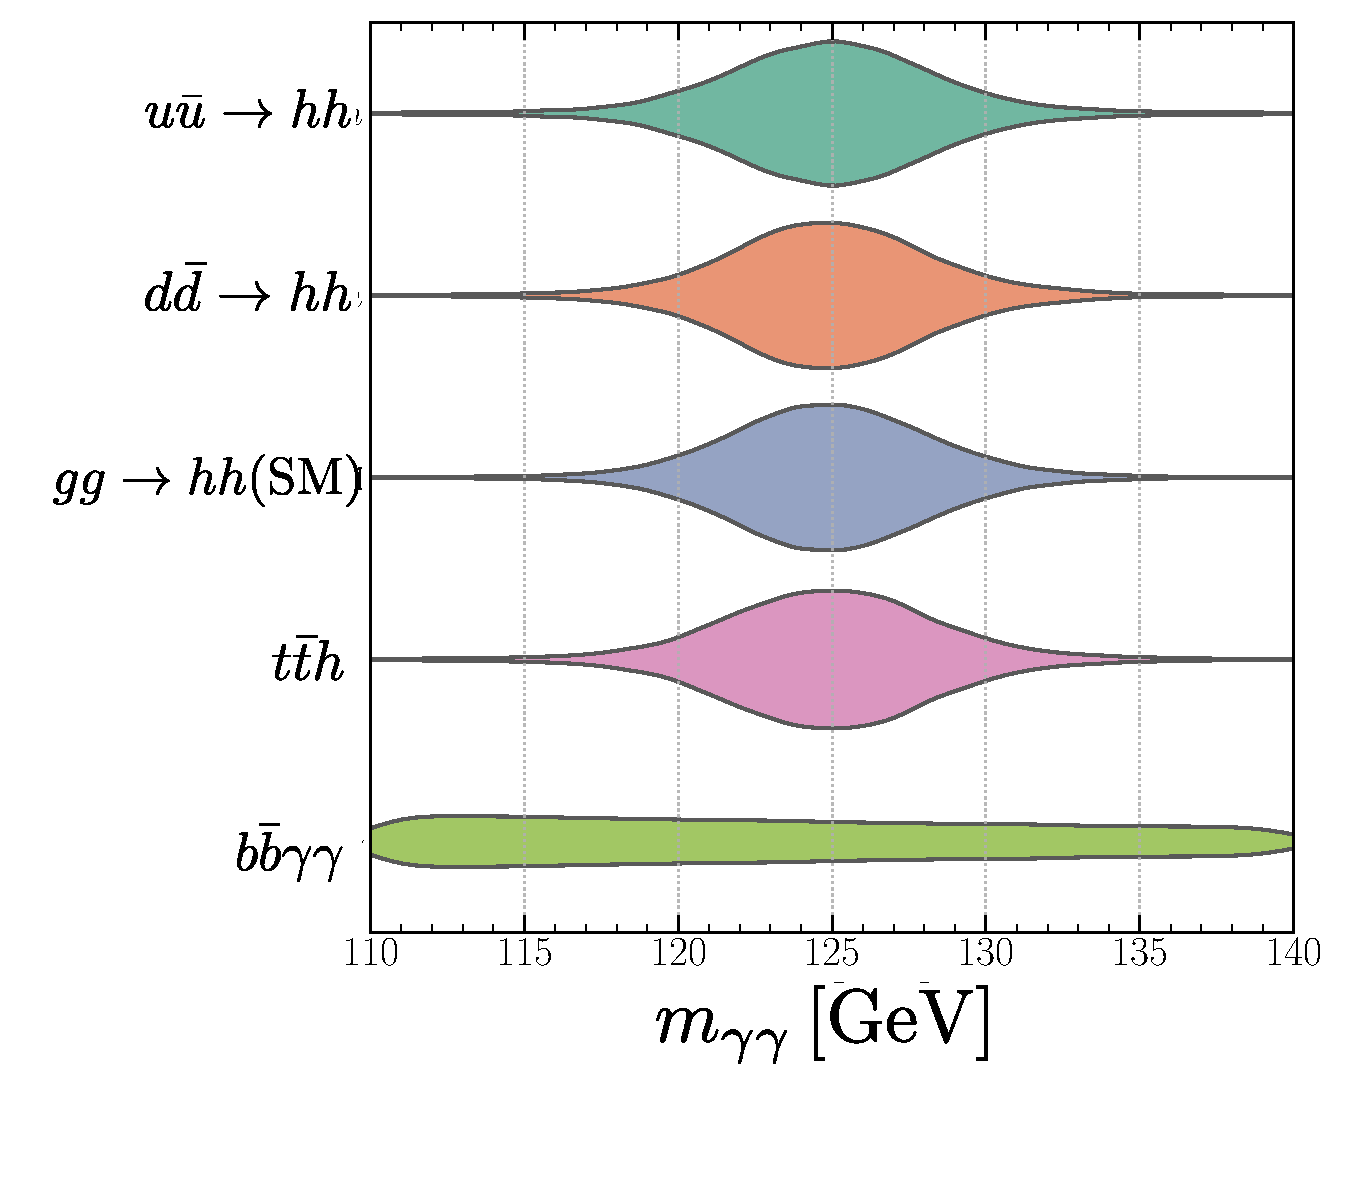
\includegraphics[width=0.35\textwidth]{fig/shape-MAA} 	\hspace*{0.25 cm}
	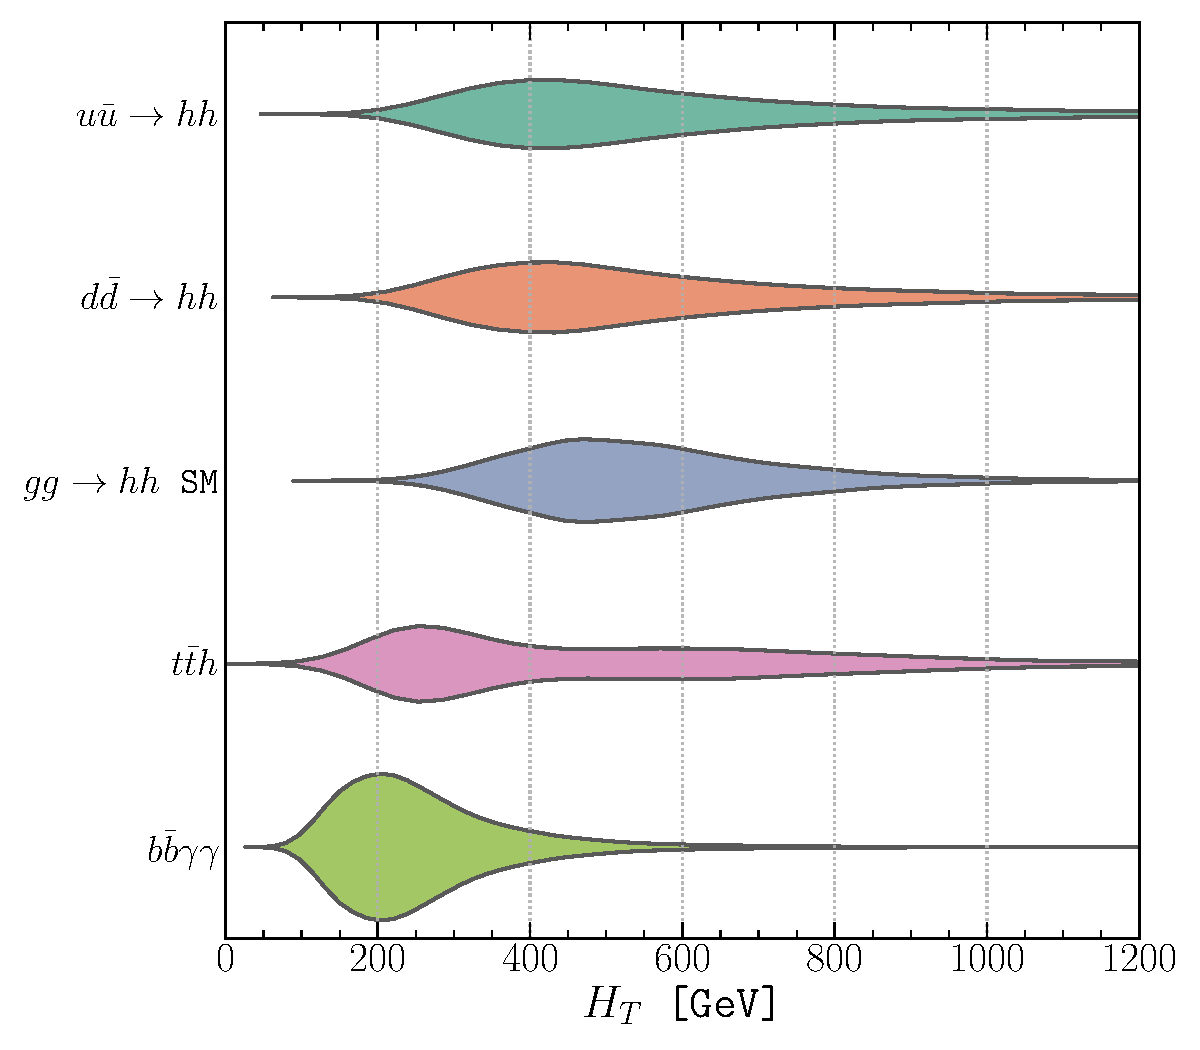
\includegraphics[width=0.35\textwidth]{fig/shape-HT}  \\
	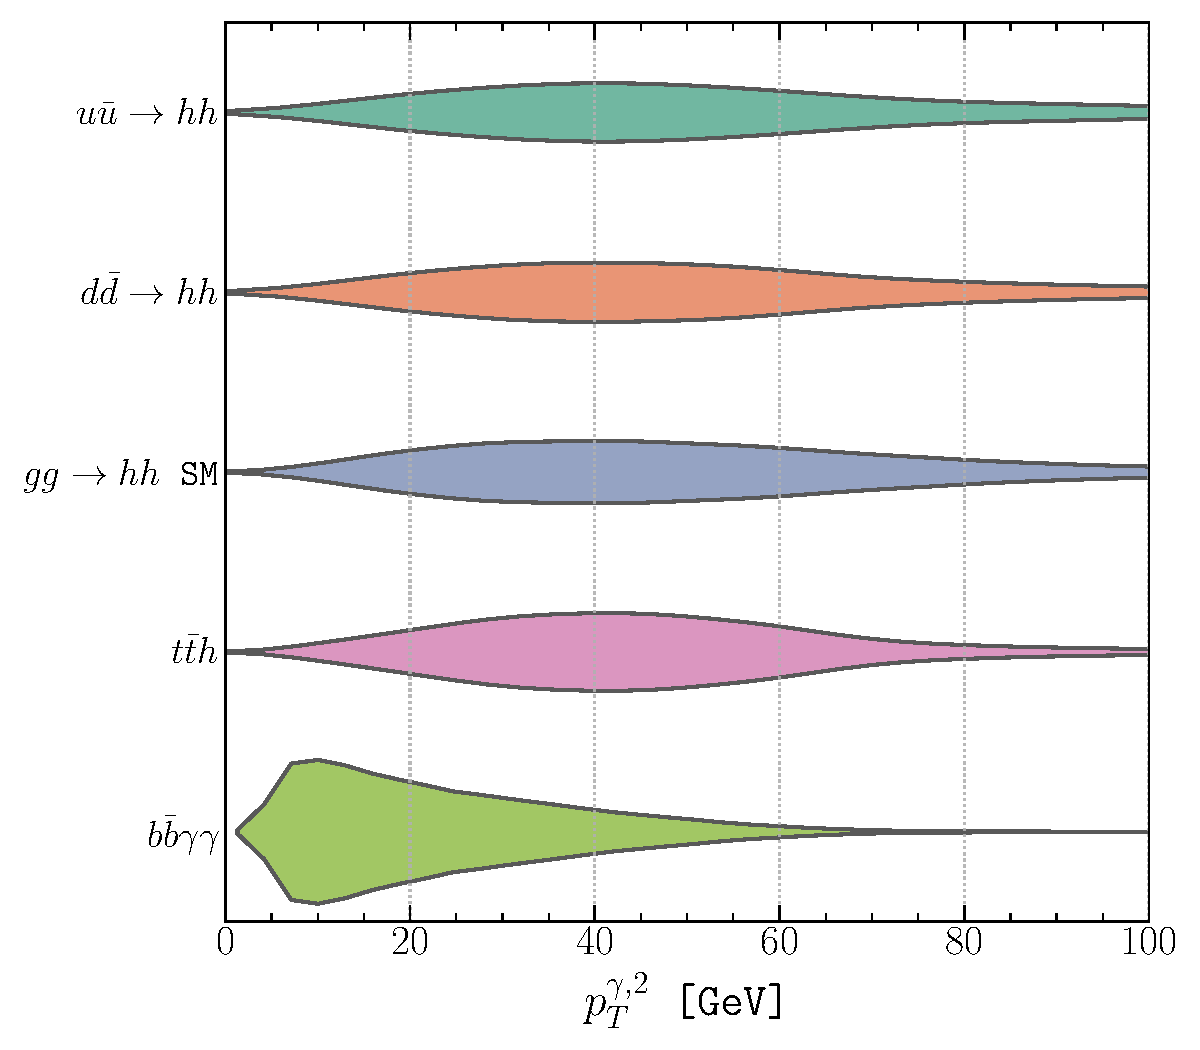
\includegraphics[width=0.35\textwidth]{fig/shape-PTA2} \hspace*{0.25 cm}
	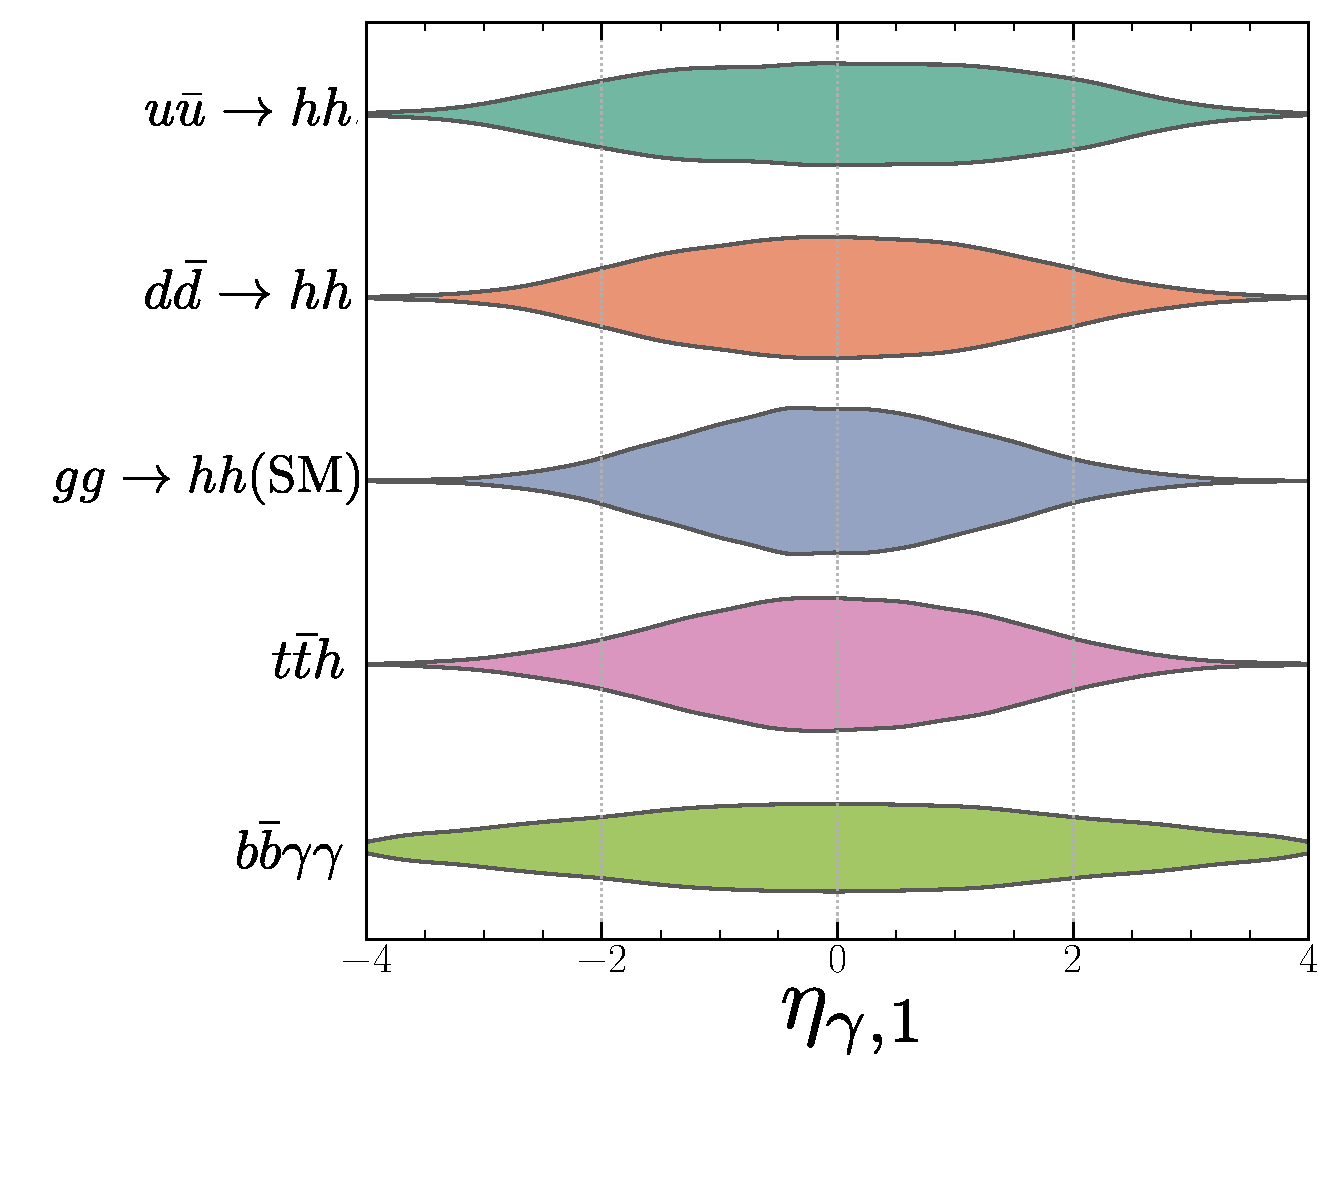
\includegraphics[width=0.35\textwidth]{fig/shape-ETAa1} 
	\caption{Violin plots showing the distributions of the most significant features used by the BDT classifier for the signal channels, and the two most significant backgrounds $ b \bar b \gamma \gamma$. }
	\label{fig:voilen}
\end{figure}  
%%%%%%%%%%%%%%%%%%%%%%%%%%%%%%%
\subsection{ Exploratory network analysis}
%%%%%%%%%%%%%%%%%%%%%%%%%%%%%%%
The aim of this analysis is to explore how the kinematic variables constructed in the previous section are related to each other. Furthermore, we are interested in examining their variation across the channels.  This can be achieved by calculating the intra-feature correlations stratified according to the signal types (ggF, $\uuA$, $\ddA$ ) or a background. This correlation will play the role of the effect measure of these features across the different channels. The correlations can  be represented as network diagrams as seen in (a) of~\autoref{fig:cor-net}. The Pearson's correlation networks show some differences amongst the different signal strata.\footnote{For network plots of the backgrounds see~\cite{Grojean:2020ech}.}. These differences can be further investigated by a post-hoc hypothesis test, based on a linear mixed effects model for each pair of the features~$X_i, X_j$ stratified according to the processes ~(ggF, $\uuA$, $\ddA$ and background )~$S_k$, given as follows
\begin{equation}
	X_i = \beta_{ij} X_j + \beta_k S_k + \beta_0,
	\label{gemisteseffekt}
\end{equation}
where $\beta_{ij}$, $\beta_k$ and $\beta_0$ are the constants for the fit. The hypothesis test is therefore preformed by taking  the ratio of log likelihood for the linear model of eq.~\eqref{gemisteseffekt}, defined as
\begin{equation}
	t = \frac{\mathscr{L} (\beta_{ij},\beta_k,\beta_0) }{\mathscr{L}(\beta_{ij},\beta_k=0,\beta_0)}.
\end{equation}
This analysis of variation~(ANOVA) yields a $p$-value for each feature pair, these $p$-values are false discovery rate~(FDR) corrected, and the correlation difference amongst the strata is considered significant if the FDR-corrected $p$-values pass the threshold $ p<0.001$ or $p>0.01$ when comparing $\uuA$ against $\ddA$.~\footnote{The threshold for this comparison is related due to the high degree of similarity between the two channels.} The result of these comparisons can be seen in sub-figures (b). We can see that many of the features do not have significant variation across the strata. This indicates that these features are not important in separating the signal from the background. The most significant variation is between the ggF (equivalently $\qqA$) and the background. While for the $\qqA$ channels, the correlation patterns are almost identical except for the correlation between the observables related to the PDFs, which is expected since the only kinematic difference between the up-and down-initiated $\qqA$ emerges from the PDFs of the up and down quarks. \\
\begin{figure}[h!]
	\centering
	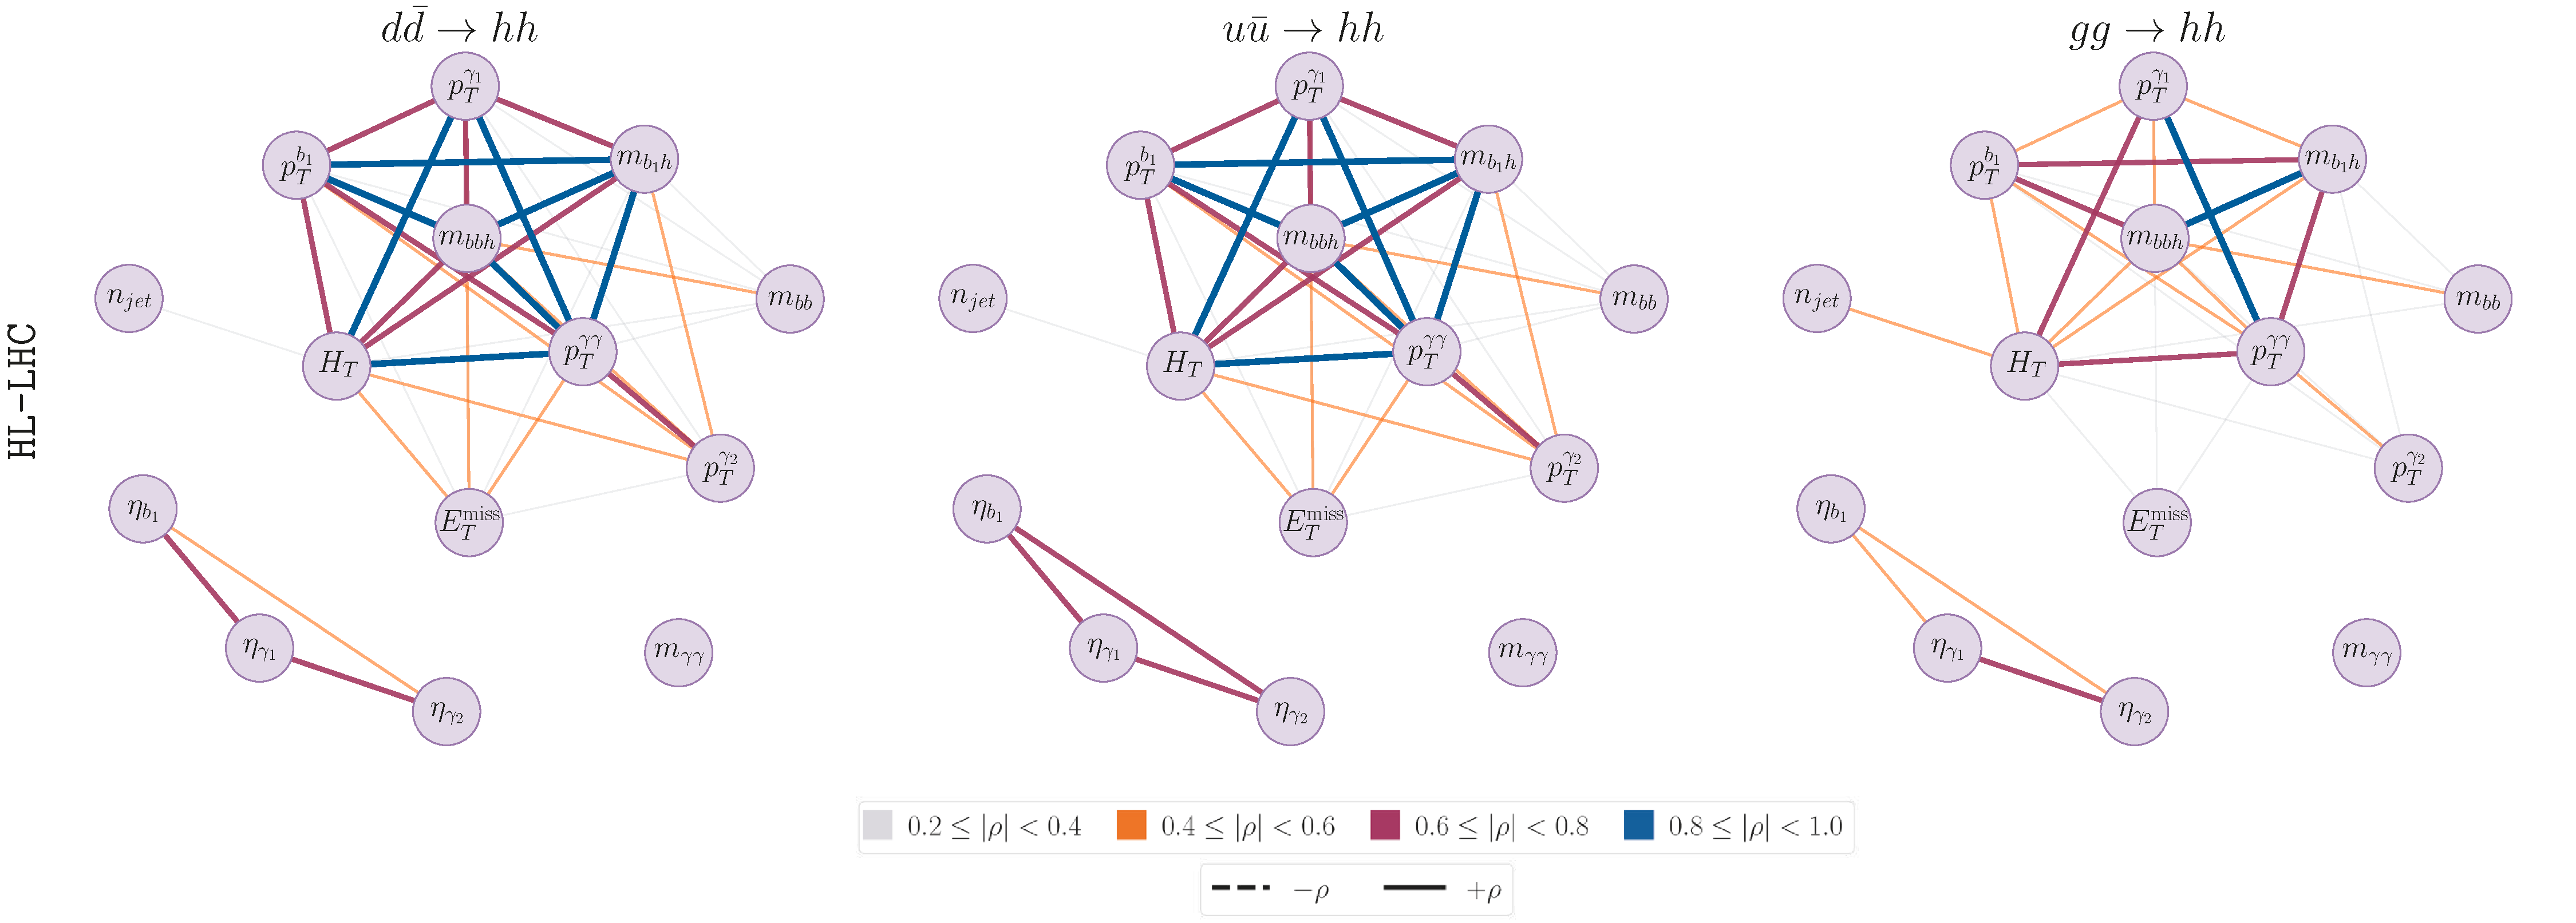
\includegraphics[width=0.9\linewidth]{fig/netzwerk/networks-signal-HL-LHC}\\
	\vspace{-0.2 cm}
	{  \footnotesize  (a)}\\
	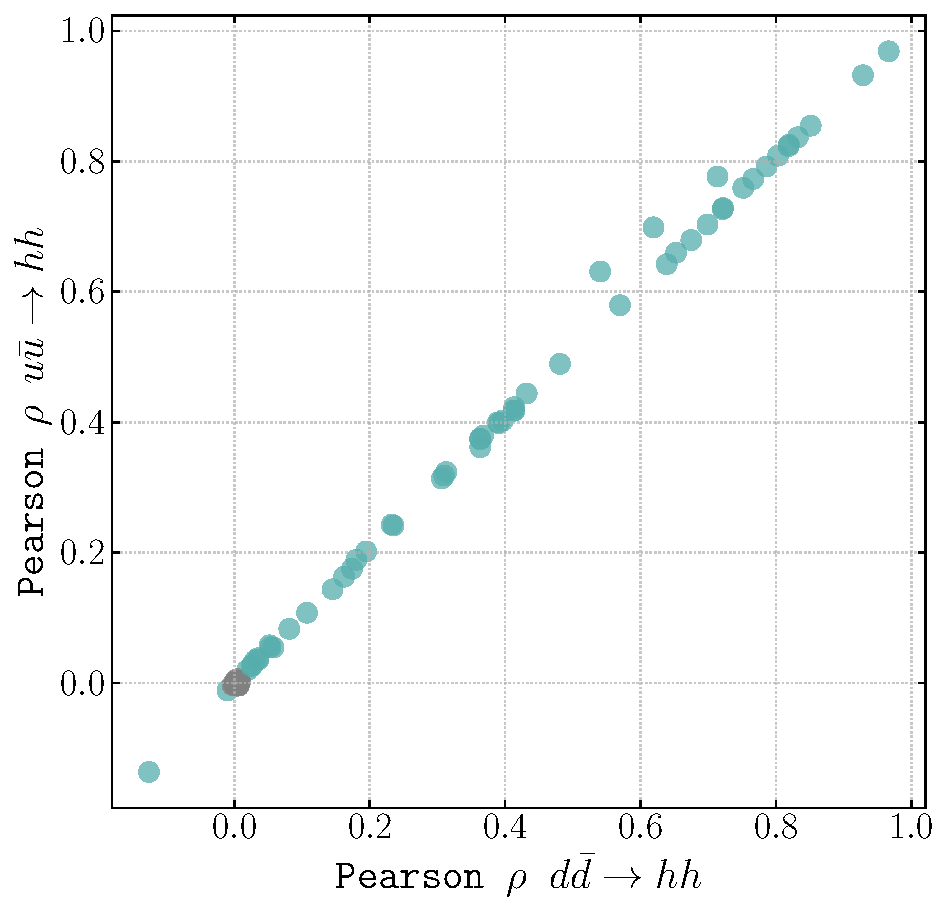
\includegraphics[width=0.45\linewidth]{fig/netzwerk/corr-ku-kd}
	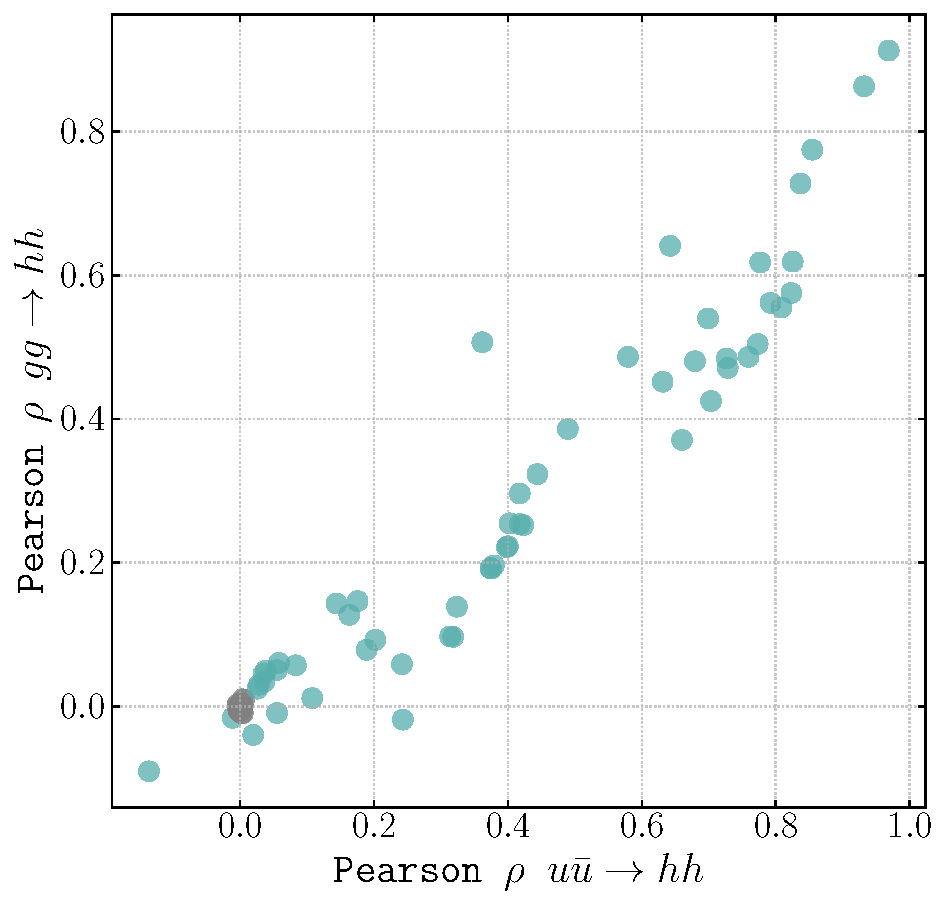
\includegraphics[width=0.45\linewidth]{fig/netzwerk/corr-ggF-ku} 
	%	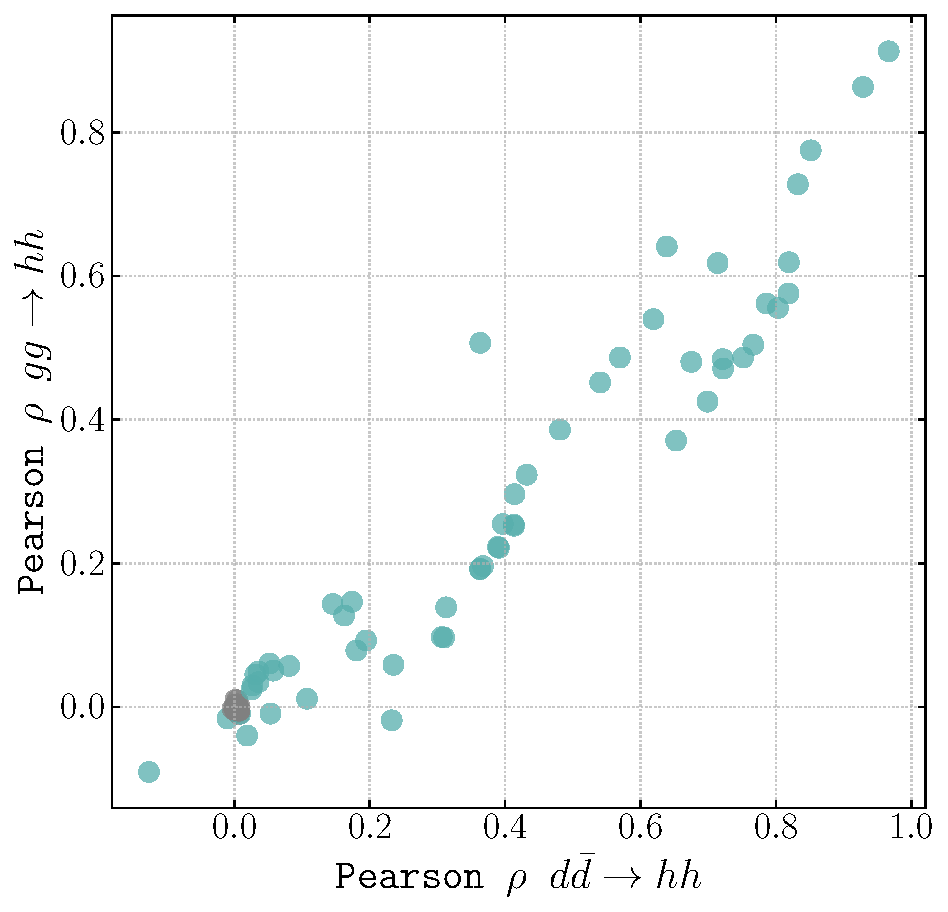
\includegraphics[width=0.29\linewidth]{fig/netzwerk/corr-ggF-kd}
	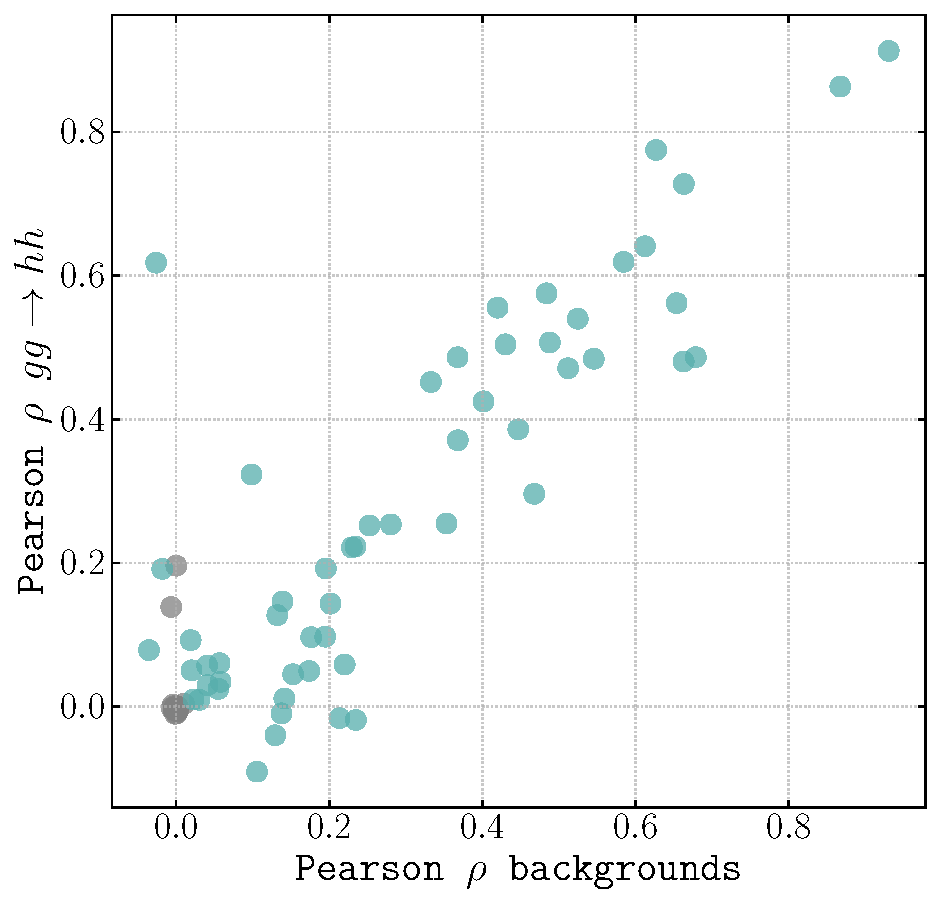
\includegraphics[width=0.45\linewidth]{fig/netzwerk/corr-ggF-bkg}\\
	{  \footnotesize  (b)}\\
	%	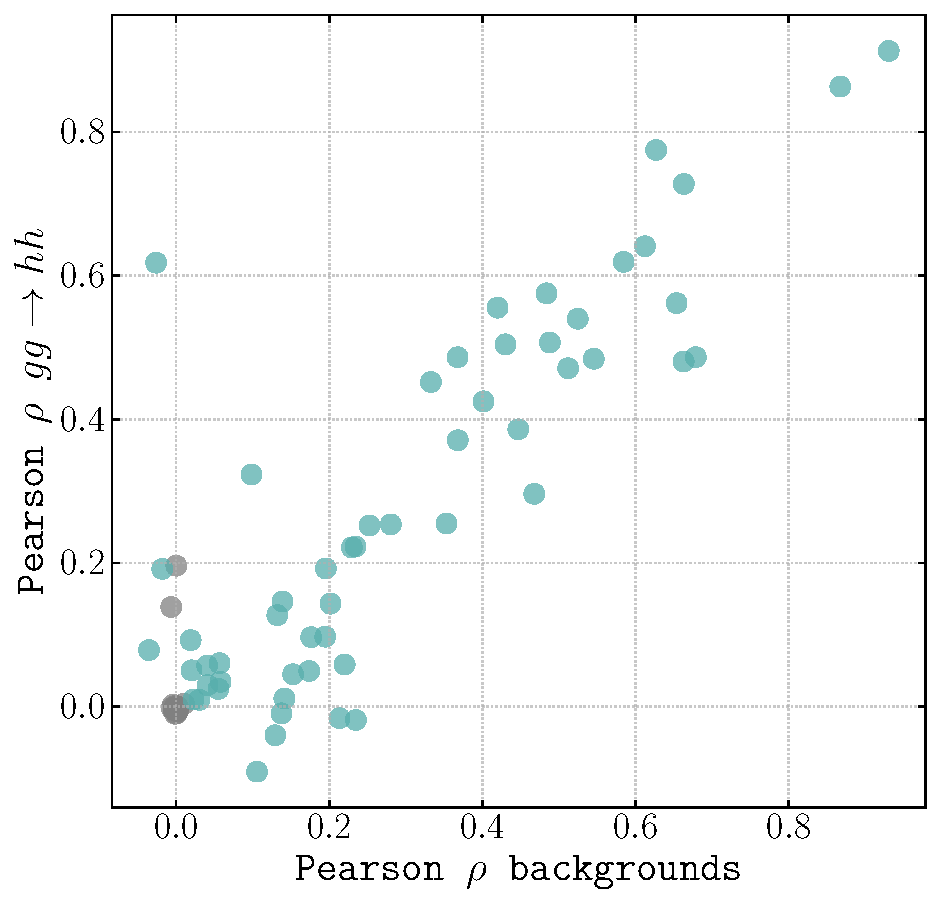
\includegraphics[width=0.375\linewidth]{fig/netzwerk/corr-ggF-bkg}
%	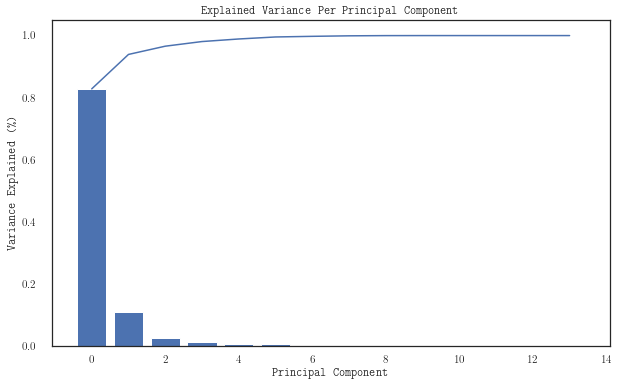
\includegraphics[height=0.25\textheight]{fig/netzwerk/download}
%	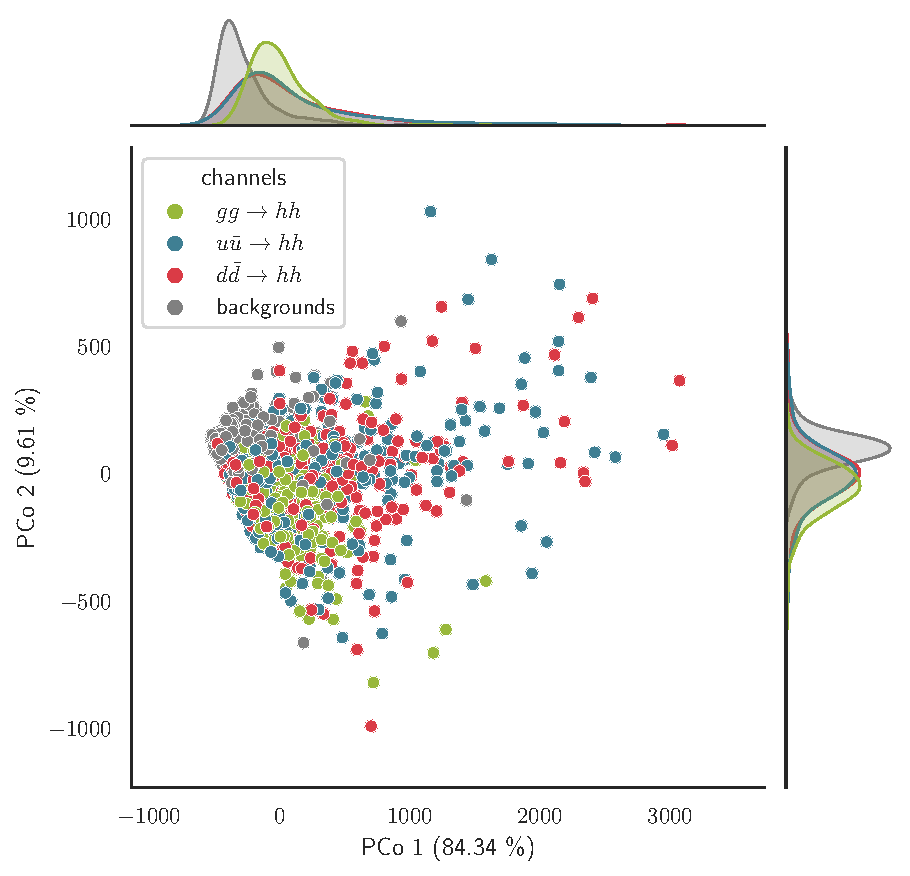
\includegraphics[height=0.25\textheight]{fig/netzwerk/pca_unsupervised-1}\\
%	\hspace{.8 cm} 			  { \footnotesize  (c)}    \hspace{6. cm}        { \footnotesize  (d)} 
	\caption{(a) Network diagrams of the signal channels of their Pearson correlation ($\rho$) between the features, showing slightly different patterns of correlation amongst these channels. (b) The same  Pearson correlations of figure (a) plotted against each other for the different signals, with the colouring indicating whether the difference between the correlation passes the hypothesis testing (ANOVA) passes the threshold  FDR-corrected $p$-value indicated at each figure.
		% (c) Scree plot of the Principal-component clustering (PCo) of the the signal channels and the backgrounds, almost full variance coverage is obtained by the first four PCo's .(d) The clustering in the first two PCo's, one can see that even with unsupervised clustering the di-Higgs signals have a significantly different distribution than the background. However, it is hard to see a marked clustering for the different signal channels.
	}
	\label{fig:cor-net}
\end{figure}
\FloatBarrier
This network analysis gives some insight of the feature set at hand. When considering that many intra-feature correlations do not vary much across the channels as seen in (b) of~\autoref{fig:cor-net}. Such features will not play a major role in the classification procedure. 
%and the features themselves cluster into four groups according to their correlations, it is tempting to further reduce the dimensionality of the feature space by preforming an unsupervised clustering via Principle Component analysis~(PCoA). Panel (c) in ~\autoref{fig:cor-net} contains a scree plot showing that the variance explained by the first few PCo's is very high, thus reducing the dimensionality of our feature space significantly. When the first two PCo's are plotted in the panel (d) of~\autoref{fig:cor-net}, the clustering of signal and the background channels  can be seen. The distinction between  the signals vs. backgrounds is visible, but less marked between the signal channel themselves, in particular $\uuA$ against $\ddA$ .  The first PCo contains, from highest weight to lowest, $m_{\gamma \gamma}, H_T, n_{jet}, m_{bb}$ and $p_T^{\gamma_1}$. The rest of the of features have a negligible weight. \\ It is not surprising to see these feature contribute the most in the clustering of events given how they are distributed as we have seen in~\autoref{fig:voilen}. In the next step of the analysis we will see then appear once more.
%%%%%%%%%%%%%%%%%%%%%%%%%%%%%%%
\subsection{Classification analysis }
%%%%%%%%%%%%%%%%%%%%%%%%%%%%%%%
The network analysis merely offers a method to explore how the Higgs pair signal differs from the backgrounds. It is useful to reduce the dimensionality of the feature space and offer ``hints'' on which subset of features has the highest discriminant power. However, for analysis of the sensitivity and complete resolution of the signal against backgrounds, the golden standard is rule-based machine learning. 
BDTs and random forests in particle physics analysis have been explored since the early LHC days. Nowadays, it has become widespread, and its popularity becomes evident by simply examining the particle physics literature. Many recent Higgs experimental analyses were performed using some rule-based ML algorithm. \footnote{Rule-based ML algorithms outperform deep neural networks~(DNN) in terms of simplicity of implementation and computational requirements. In addition, rule-based algorithms, such as decision trees, are more transparent as far as the signal vs.~background separation is concerned }\\
In this analysis, the extreme gradient BDT~(XGBoost), with its Python implementation~\cite{10.1145/2939672.2939785}, has been used as the classifier algorithm. The standard procedure for training and testing the classifier was followed, starting with the complete list of features listed in~\autoref{constructingfeat} and then the most important features were shortlisted to improve the efficiency and performance of the classifier. This was possible due to the introduction of interpretability to the ML analysis that provided variable importance measures, by which features with a low importance index can be removed. \\
Interpretability is achieved by incorporating a mathematically robust measure from  Game Theory known as \textbf{Shapley values}~\cite{shapley1951notes}. This measure formulates an axiomatic prescription for fairly distributing the payoff of a game amongst the players in a $n$-player cooperative game. When applied to ML, Shapley values estimate the significance of the features used in the classification. The process naturally and mathematically lends itself to examining the correlations amongst the features used in the classification since all possible combinations of variables can be taken out of the game to check the outcome. Further information regarding the application of Shapley values in particle physics analysis can be found in refs.~\cite{Grojean:2020ech,Alvestad:2021sje,Cornell:2021gut}.  The same procedure described in~\cite{Grojean:2020ech} was followed for the Higgs pair production study. The importance of a variable in determining the outcome of classification will be quantified by the mean of the absolute Shapley value, $\overline{|S_v|}$, larger values signifying higher importance. The SHAP (Shapley Additive exPlanations)~\cite{NIPS2017_7062} package implemented in Python was used. This package computes the feature importance using Shapley values calculated exactly from  tree-explainers~\cite{2018arXiv180203888L, Lundberg:2020vt}. This analysis is to be published soon~\cite{IML}\\
\subsubsection*{Classifier output}
The trained BDTs outputs are extracted as confusion matrices,  with number of events as entries. The diagonal elements of these matrices represent the true positive~(TP) identification of the signal and true negative~(TN) rejection of the background. In contrast, the upper triangular part represents the signal loss, or false-negative counts~(FN). The lower triangular part shows the remaining background contamination of the signal, or the false-positive counts ~(FP). Using these counts, it is possible to estimate the accuracy score $ACC$ of the classifiers
\begin{equation}
	ACC = \frac{TP+TN}{TP+TN+FP+FN} \approx 0.7,
\end{equation}
And the sensitivity $ TP/P \approx 0.2$, which corresponds to the $\epsilon_{SEL}$ of the cut-based analysis. Here we see that the ML-based analysis yielded a four- to five-fold increase in~ $\epsilon_{SEL}$ compared to the cut and count method. \autoref{tab:HL-LHC-confusion-CH} shows one of these matrices from the classification of the ggF SM signal separated into the topologies according to their dependence on~$C_\phi$. 
\begin{table}[]
	\centering
	{\footnotesize
		\begin{tabular}{ll|rrrrr|r}
			\multirow{7}{*}{\rb{\bf Actual no. of events\hspace{0.45cm}}} & \multicolumn{7}{c}{\bf Predicted no. of events at HL-LHC}\\
			\cmidrule[\heavyrulewidth]{2-8}
			& Channel & $\hhtri$ & $\hhtri$ &  $\hhbox$&      $\QQh$ & $\bbaa$ &   total \\
			\cline{2-8}
			&$\hhtri$         &   28 &	14 &	18&	38&	10&	108 \\
			&$\hhint$         &   	89&	80&	129&	178&	41&	517\\
			&$\hhbox$         &   77&	105&	266&	265&	50&	763 \\
			&$\QQh$           &  177&	98&	191&	5,457&	1,835& 7,758 \\
			&$\bbaa$          & 1,743&	845&	1,074& 30,849&	287,280&	321,791 \\
			%	\cline{2-8}
			%	&$\mathcal{Z}_j$& 0.61&	2.37&	6.49&	28.45&	534.1	&       \\
			\cmidrule[\heavyrulewidth]{2-8}
		\end{tabular}
	} 
	\caption{The confusion matrix output of the trained BDT  five-channel classifier. The separation between the ggF topologies allows for setting constraints on $C_\phi$. The events shown are for the HL-LHC at 14 TeV and integrated luminosity of 6$\iab$, assuming the SM signal.}
	\label{tab:HL-LHC-confusion-CH}
\end{table}
For up- and down-quark $ \qqA$, the same matrices were constructed, and since the number of events for these processes scale with $C_{q\phi}^2$, it is only required to produce one confusion matrix for each classification procedure, like the case of the ggF channel. \\ For the fitting procedure, a Bayesian framework based on an MCMC method was used, analogous to the procedure described in~\autoref{sec:fit}. \\  The full analysis code, including the BDT training and fits as well as the confusion matrices for the classification procedures performed can be found in the~\texttt{Github} repository: \href{https://github.com/talismanbrandi/IML-diHiggs.git}{https://github.com/talismanbrandi/IML-diHiggs.git}. 
\begin{figure}[t!]
	\centering
	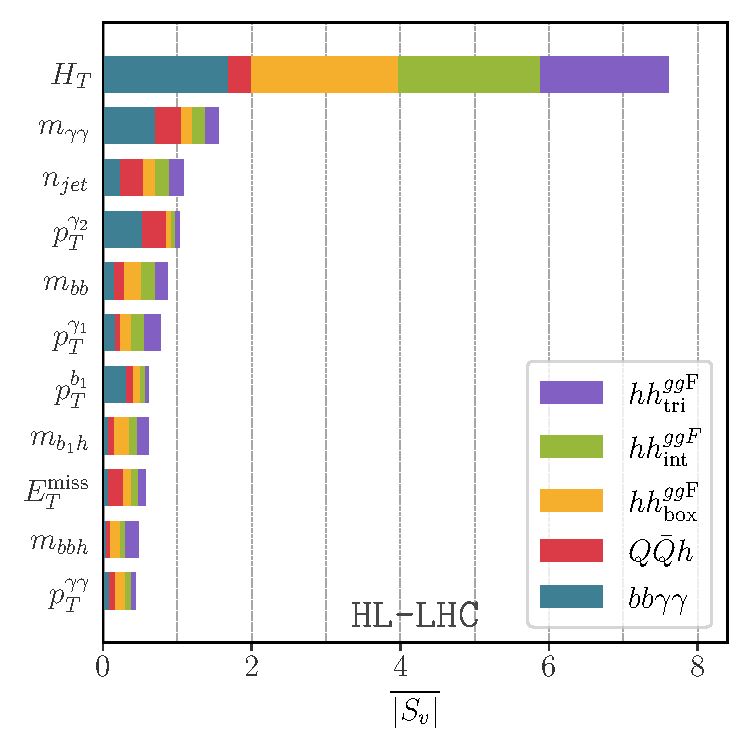
\includegraphics[width=0.4\linewidth]{fig/HL-LHC-shap-bbxaa-bbh-tth-hhsm.pdf}
	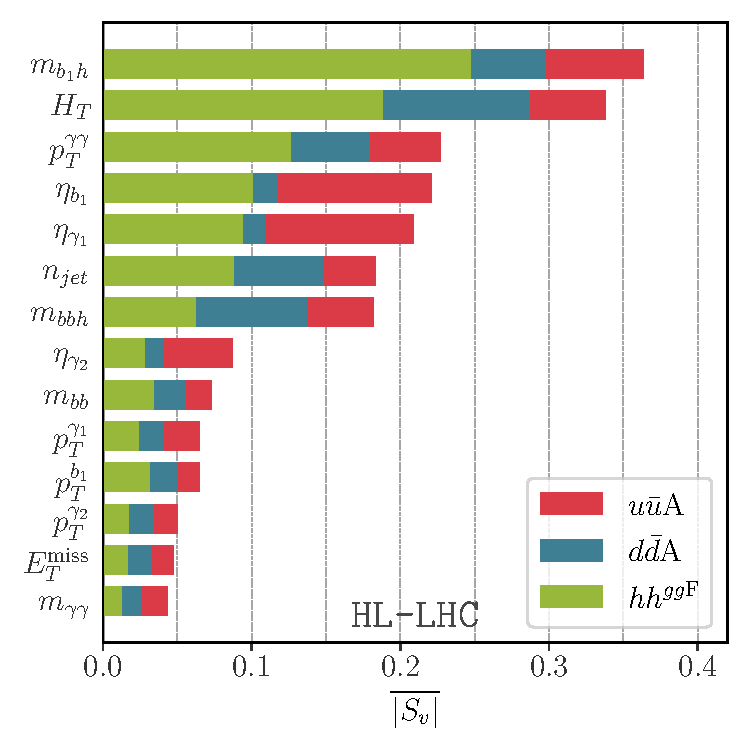
\includegraphics[width=0.4\linewidth]{fig/HL-LHC-shap-ku-kd-hhsm.pdf}\\
	\hspace{.5 cm} 			  { \footnotesize  (a)}    \hspace{5. cm}        { \footnotesize  (b)}  \\
	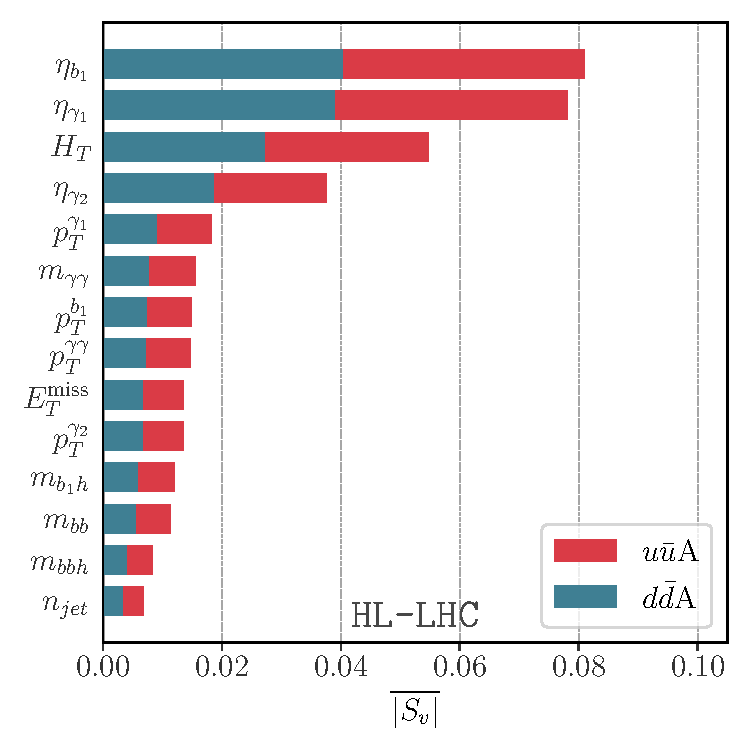
\includegraphics[width=0.4\linewidth]{fig/HL-LHC-shap-ku-kd.pdf}\\
	{  \footnotesize  (c)}
	\caption{The feature importance output in terms of $\overline{|S_v|}$. The higher the value of $\overline{|S_v|}$, the more important the kinematic variable is in separating the different channels : (a) The hierarchy of variables important for the separation of $\hhtri$ from $\hhint$ events from $\hhbox$, $\QQh$ and $\bbaa$ QCD-QED background  (b) The hierarchy of variables important for the separation of $hh^{gg\rm F}$, $\uuA$ and $\ddA$ events. (c) The hierarchy of variables important for the separation of $\uuA$ from $\ddA$ events.}
	\label{fig:shap}
\end{figure}
\FloatBarrier
\subsubsection*{Feature importance and Shapley values}
Another output of the interpretable BDT is the SHAP scores for the features used in the classification.  The $\overline{|S_v|}$ values are used to order the features used for the classification. The most important features in different classifiers used in this analysis is seen in~\autoref{fig:shap}. Panel (a) shows the hierarchy of the features used for the separation of the SM ggF signal from the backgrounds. The BDT was able to distinguish between the different signals, a task cut-based analysis or unsupervised clustering are unable to fructify. Panel (b) shows the list of feature importance for the ggF vs $\qqA$ classification, while (c) demonstrates the full strength of the BDT in distinguishing $\uuA$ from $\ddA$ despite having very little variation of their kinematic distributions.  As expected, $\uuA$ vs $\ddA$ classification, the features appeared on top of the list, are related to the different PDF's but their ranking was unintuitive because this classification is a genuine a multivariate problem, where the intra-variable correlations and differences have been fully extorted. 
%%%%%%%%%%%%%%%%%%%%%%%%%%%%%%%
\section{Fit results\label{sec:resultsly}}
%%%%%%%%%%%%%%%%%%%%%%%%%%%%%%%
The fit from the cut-bases analysis was originally made for 3$\inab$ and published in~\cite{Alasfar:2019pmn}. For a better comparison with the optimised BDT multivariate analysis, the fit for this thesis was carried out again for 6$\inab$, and with SMEFT Wilson coefficient parametrisation, thus harmonising it with the results of the other chapters. The fits were done in the $C_\phi-C_{q\phi}$ plane shown the top plots of~\autoref{fig:rescut}. As well as the $C_{u\phi}-C_{d\phi}$ one in the low panel of the same figure.  We see that even with the traditional technique, two-parameter fits were possible. However, the bounds obtained on the trilinear self-coupling modifier are weaker than the projected bounds for the HL-LHC, made by ATLAS and CMS~\cite{ATL-PHYS-PUB-2018-053, ATLAS:2018rvj,CMS-PAS-FTR-18-011}, which is expected due to the dilution of these bounds by adding light Yukawa coupling modifiers and the loss of some signal due to the analysis technique. For the $C_{u\phi}-C_{d\phi}$ combined fit, no correlation between the two parameters is seen. \\ To demonstrate the power of multivariate~(MV) analysis, we compare the fit results from single parameter fits of this analysis to the cut-and count technique~(CC) for both up and down quark coupling modifiers at 68\% CL/CI 
\begin{eqnarray}
	C_{u\phi}^{MV} \left(\kappa_u^{MV}\right) = [-0.09, 0.10] \;([-466, 454]),\quad C_{u\phi}^{CC} (\kappa_u^{CC}) = [-0.18, 0.17] \;([-841, 820]), \nonumber\\
	C_{d\phi}^{MV} (\kappa_d^{MV}) = [-0.16, 0.16] \;([-360, 360]),\quad C_{d\phi}^{CC} (\kappa_d^{CC}) = [-0.18, 0.18] \;([-405, 405]). \nonumber\\
\end{eqnarray}
\begin{figure}[htpb!]
	\centering
	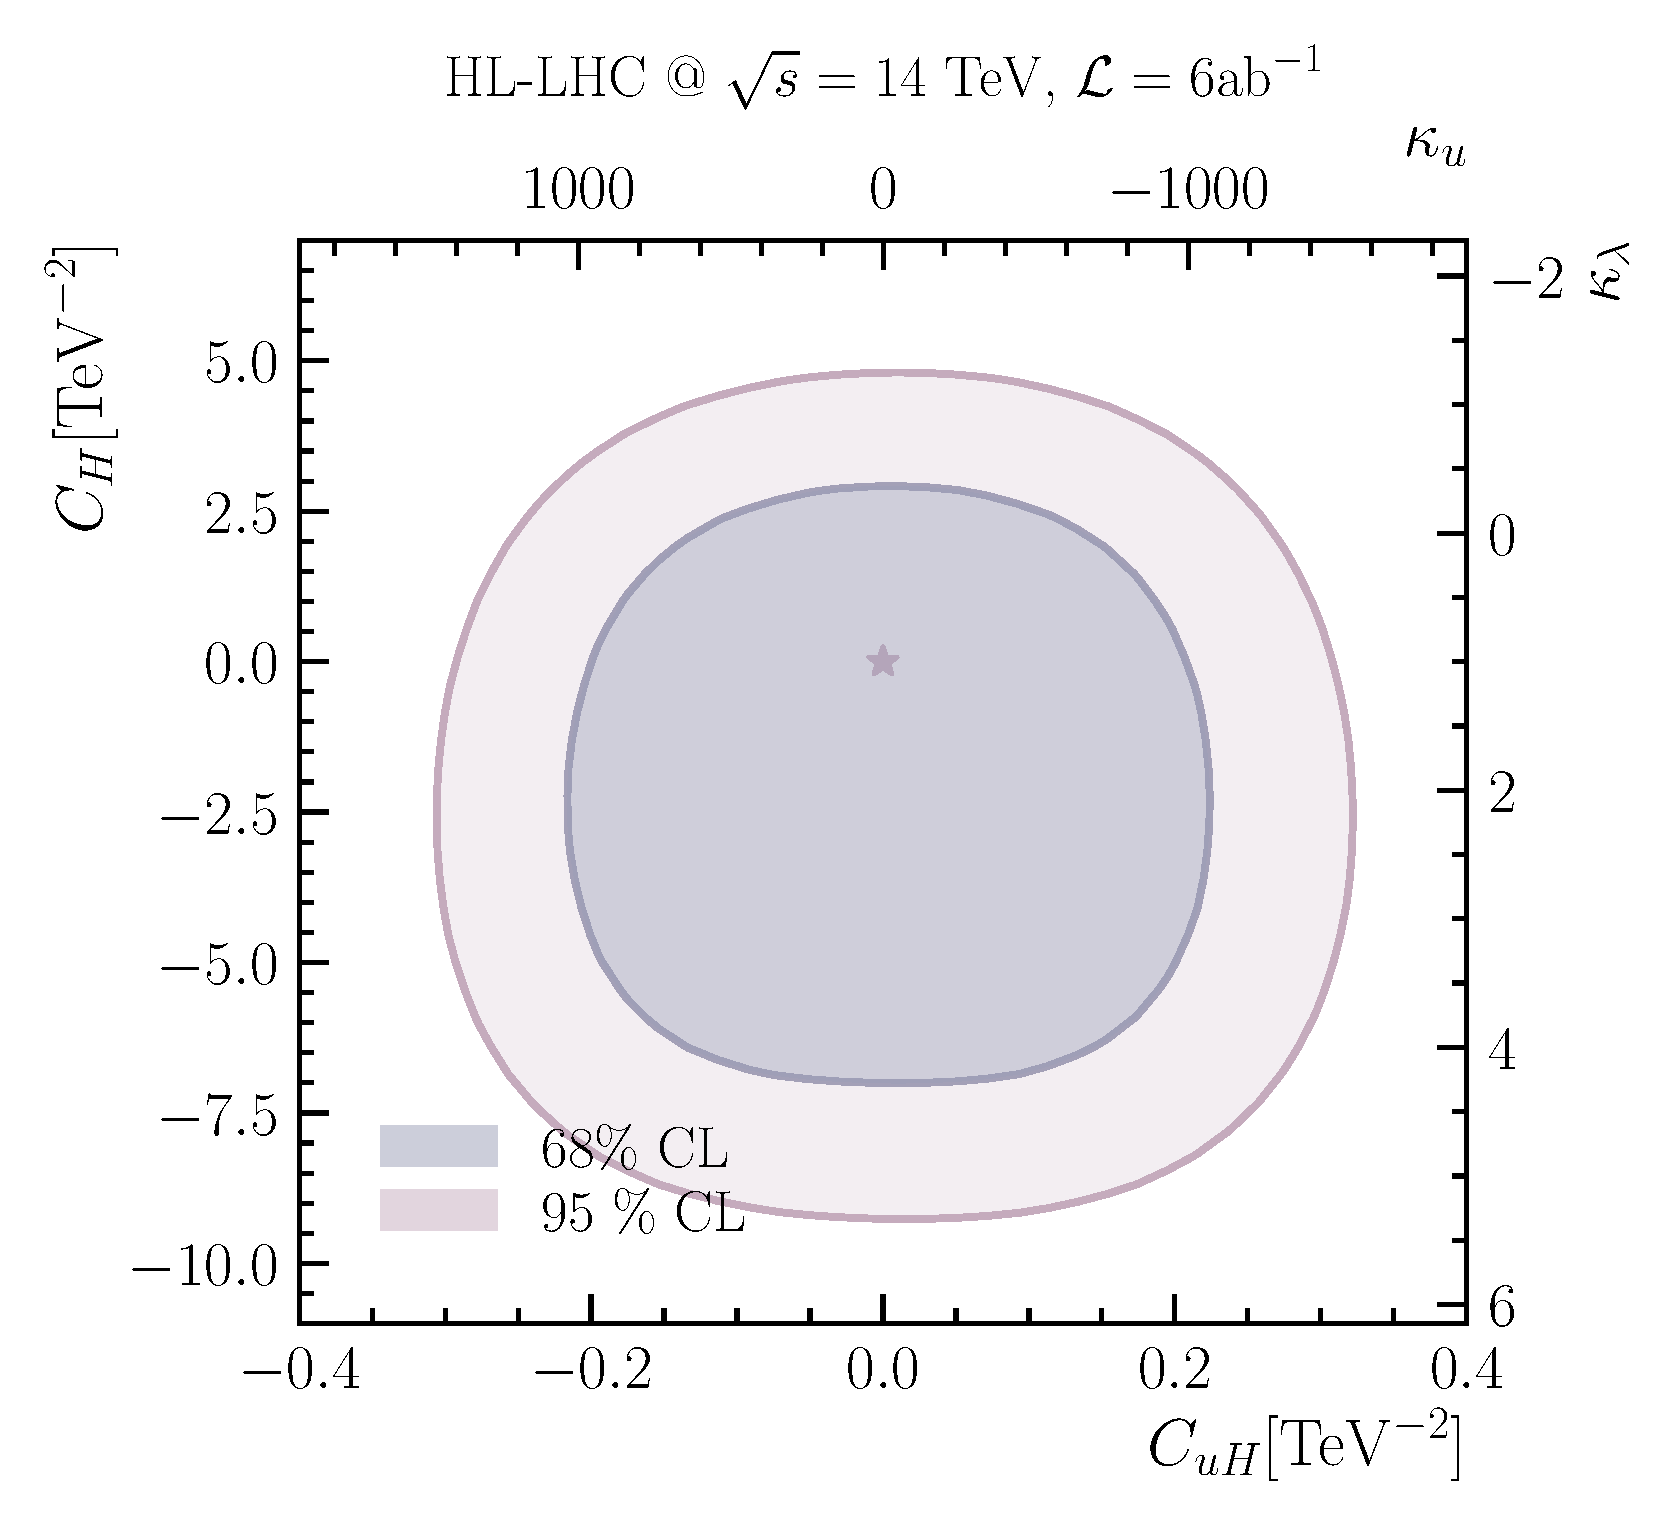
\includegraphics[width=0.46\textwidth]{fig/kukl-HL-LHC} % \hspace*{0.25 cm}
	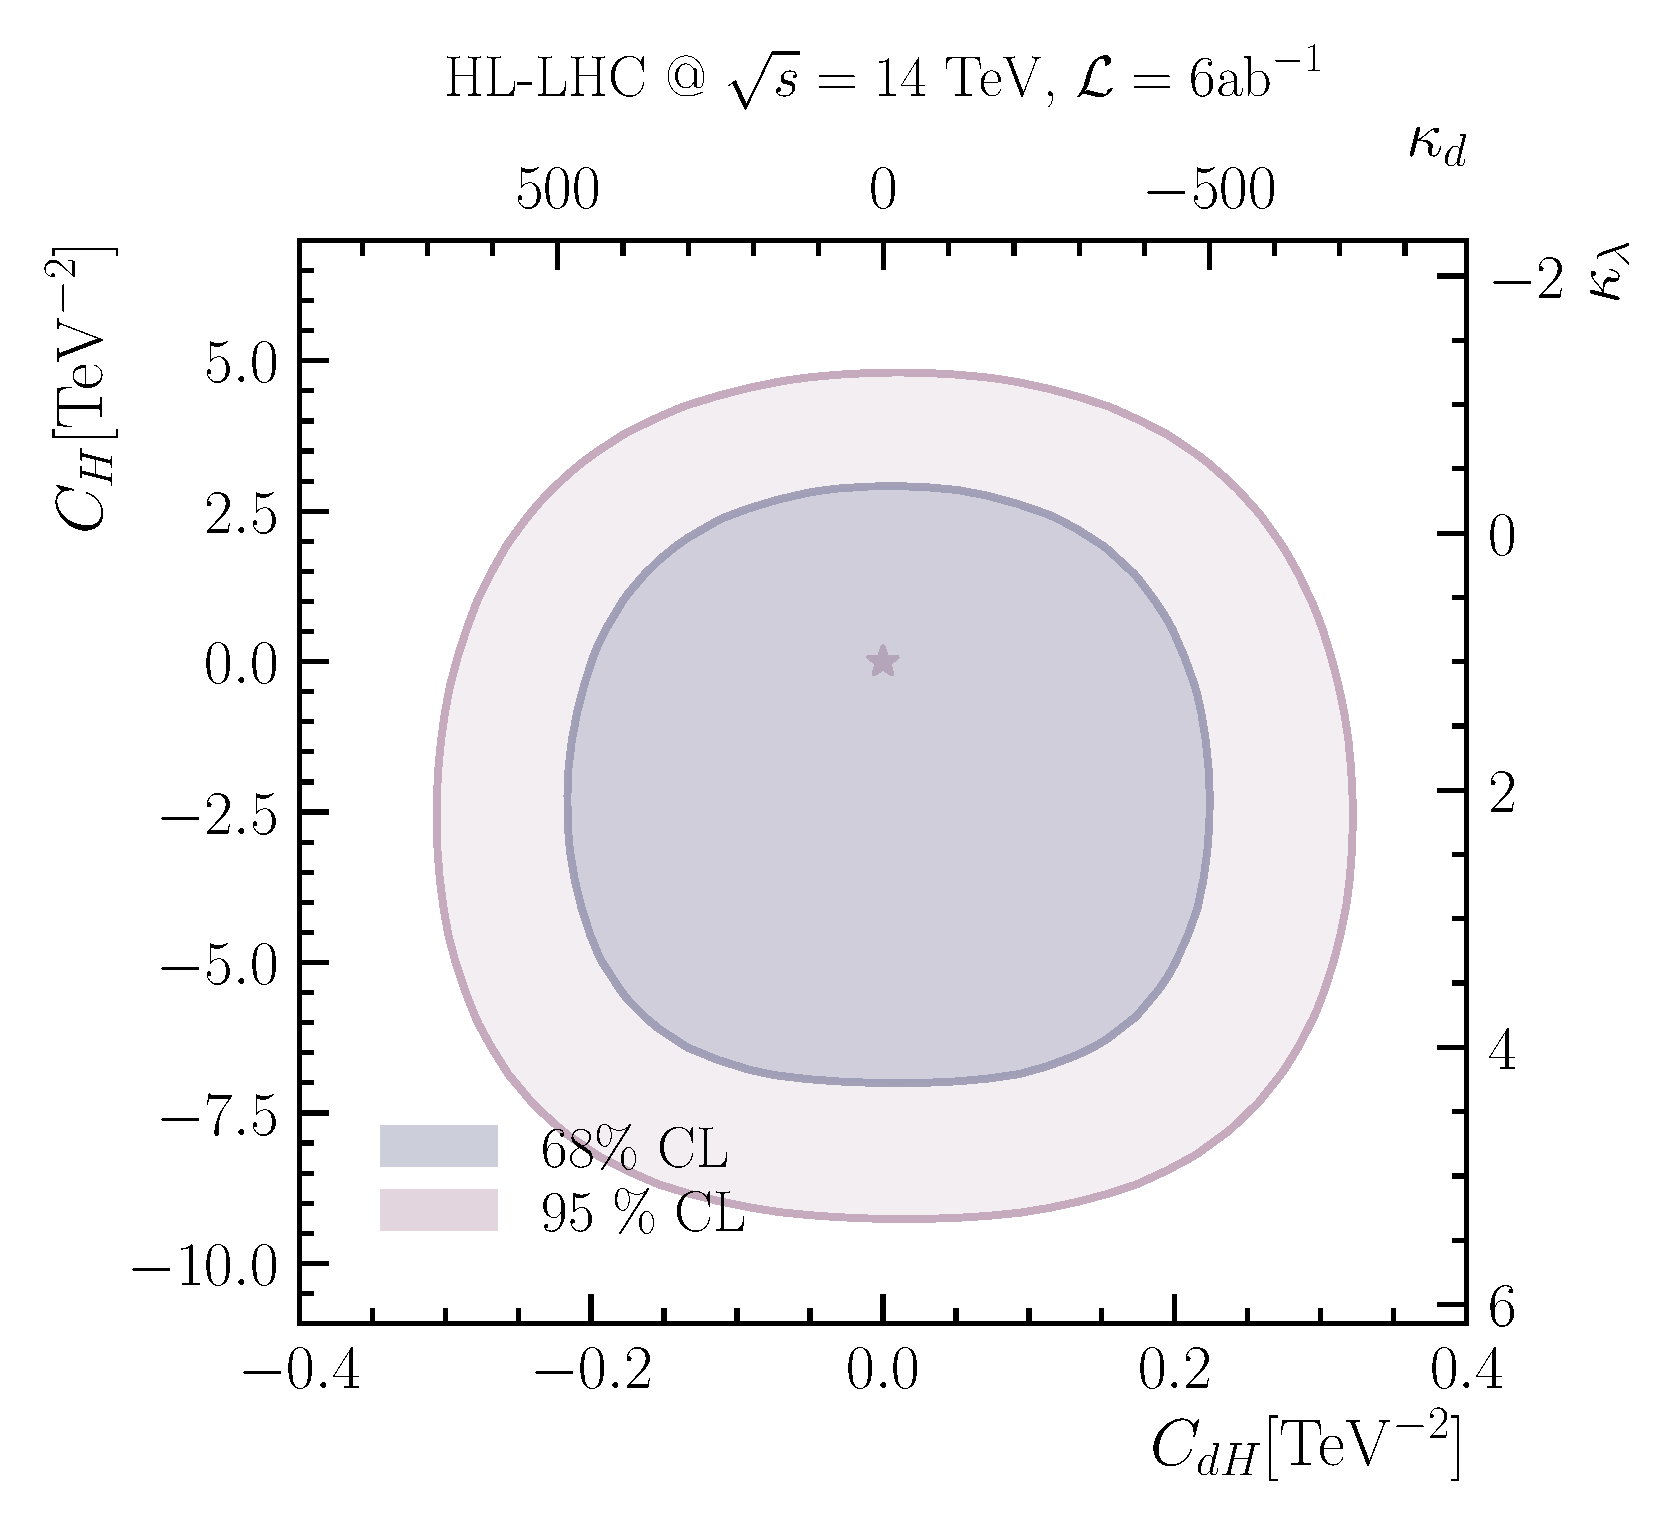
\includegraphics[width=0.46\textwidth]{fig/kdkl-HL-LHC} 
	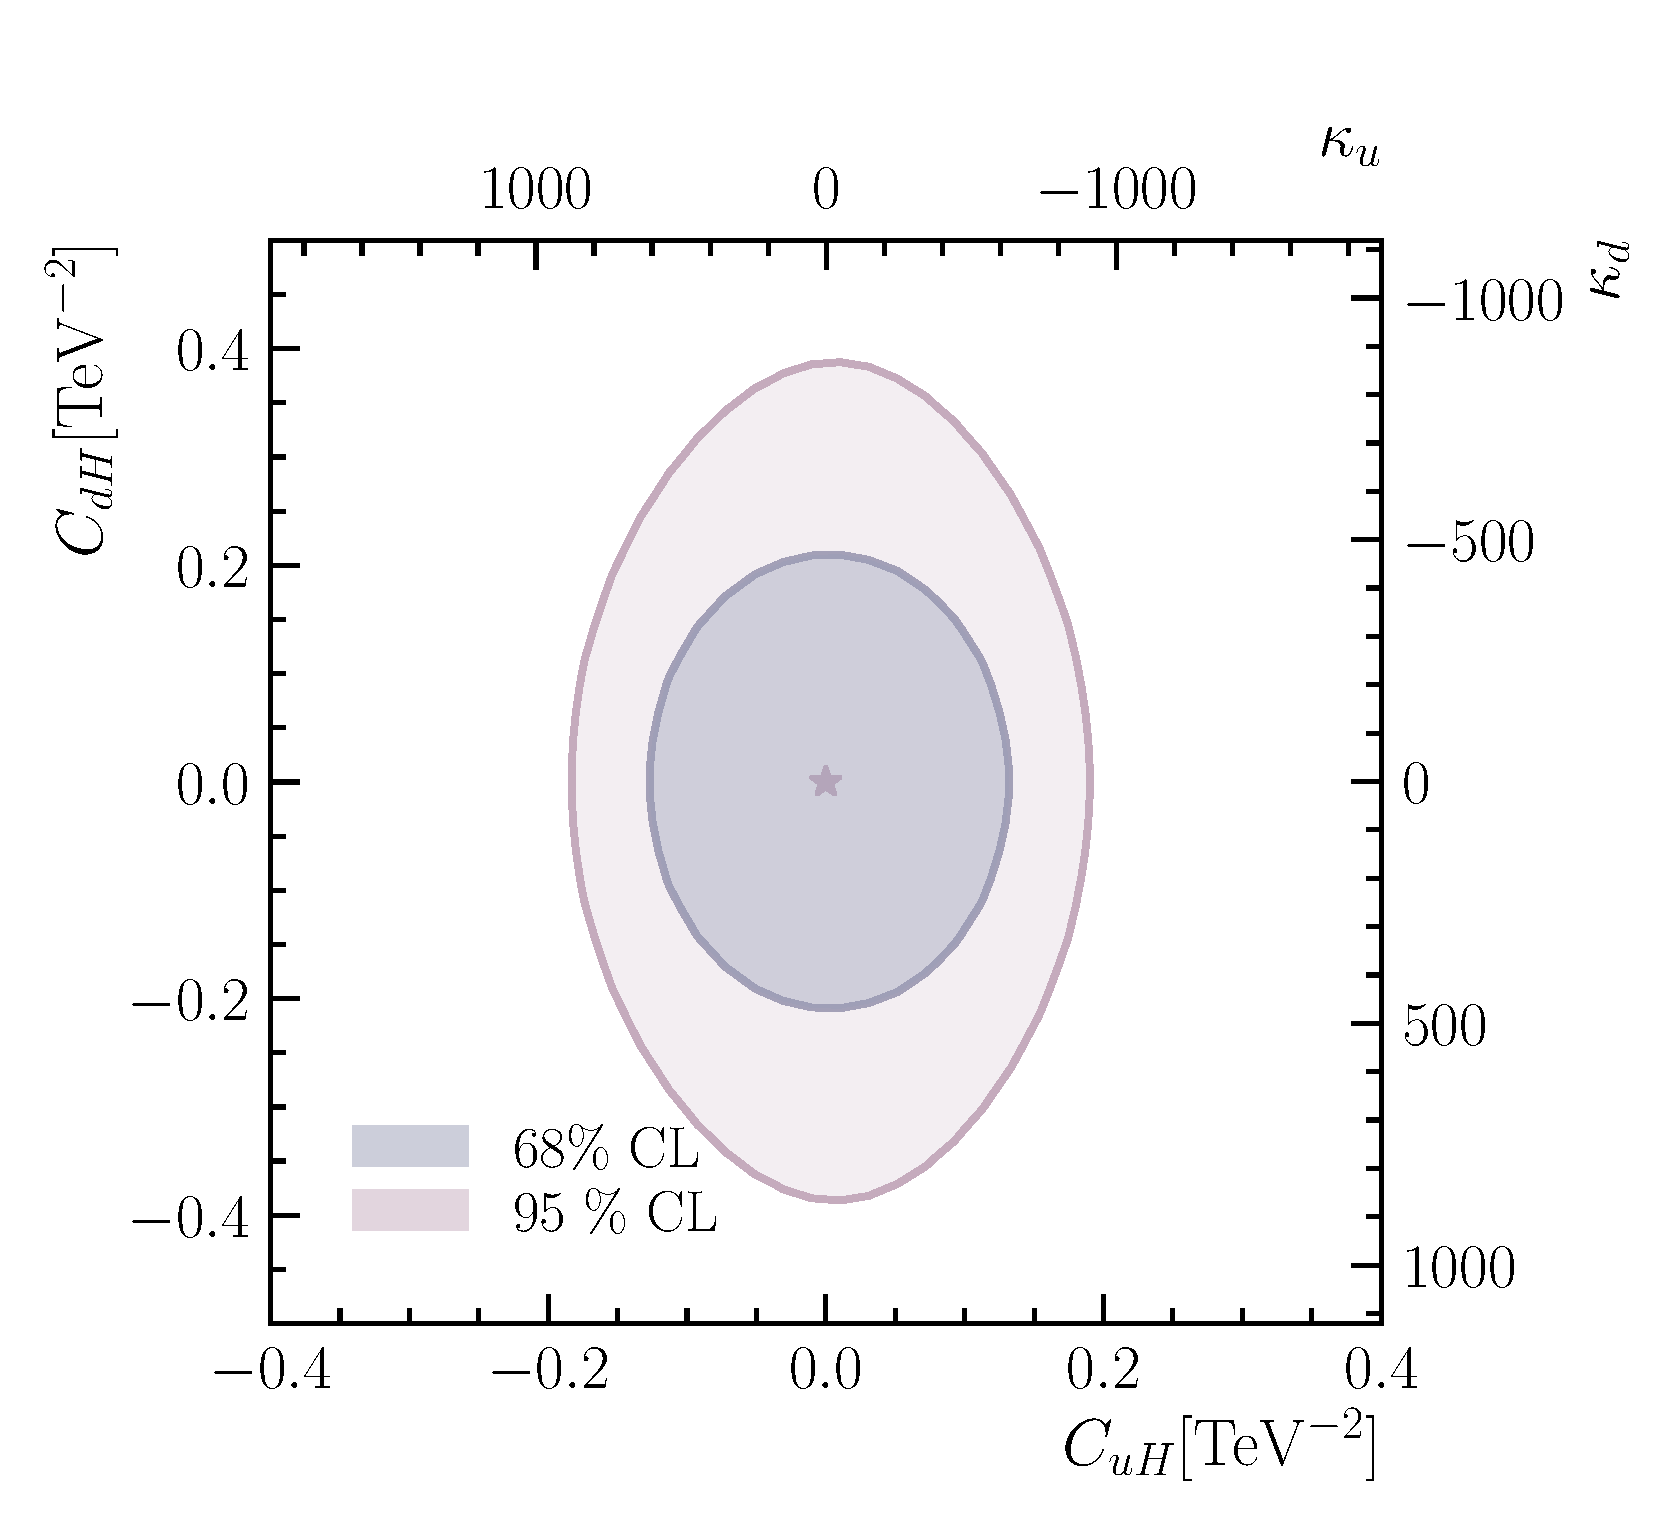
\includegraphics[width=0.46\textwidth]{fig/kdku-HL-LHC}  \\
	\caption{The  68\% and 95\% CL contours of the constraints on up and down Yukawa coupling modifiers as well as $C_\phi$ from two-parameter fits using the results of the cut-based analysis for the HL-LHC at 14 TeV and $6 \invab$ integrated luminosity. }
	\label{fig:rescut}
\end{figure}  
A significant improvement of the bounds from using MV analysis over CC one of two-fold for $C_{u \phi}$,  but a mild one for $C_{d\phi}$ with $\mathcal O(10\%)$ improvement.\\ 

To compare the ML multivariate analysis used to other sensitivity projections, the projections on the trilinear coupling modifier $C_\phi$ are shown in~\autoref{fig:constraintkl}. These bounds are obtained by using a BDT classification showcased in~\autoref{tab:HL-LHC-confusion-CH}, by showing the significance~$\mathcal Z = \sqrt{q_\mu}$ functions for the linear, quadratic and combined dependence on $C_\phi$. The constraints that we have obtained here are similar to or slightly better than the results quoted by the experimental sensitivity analysis quoted before. This was achieved by optimising the BDT by separating the signal and background channels, as well as the exclusion of less-important features. The projected $1\sigma$ bound on $C_\phi$ is $[-1.57, 1.00]$ at HL-LHC. 
\begin{figure}[h!]
	\centering
	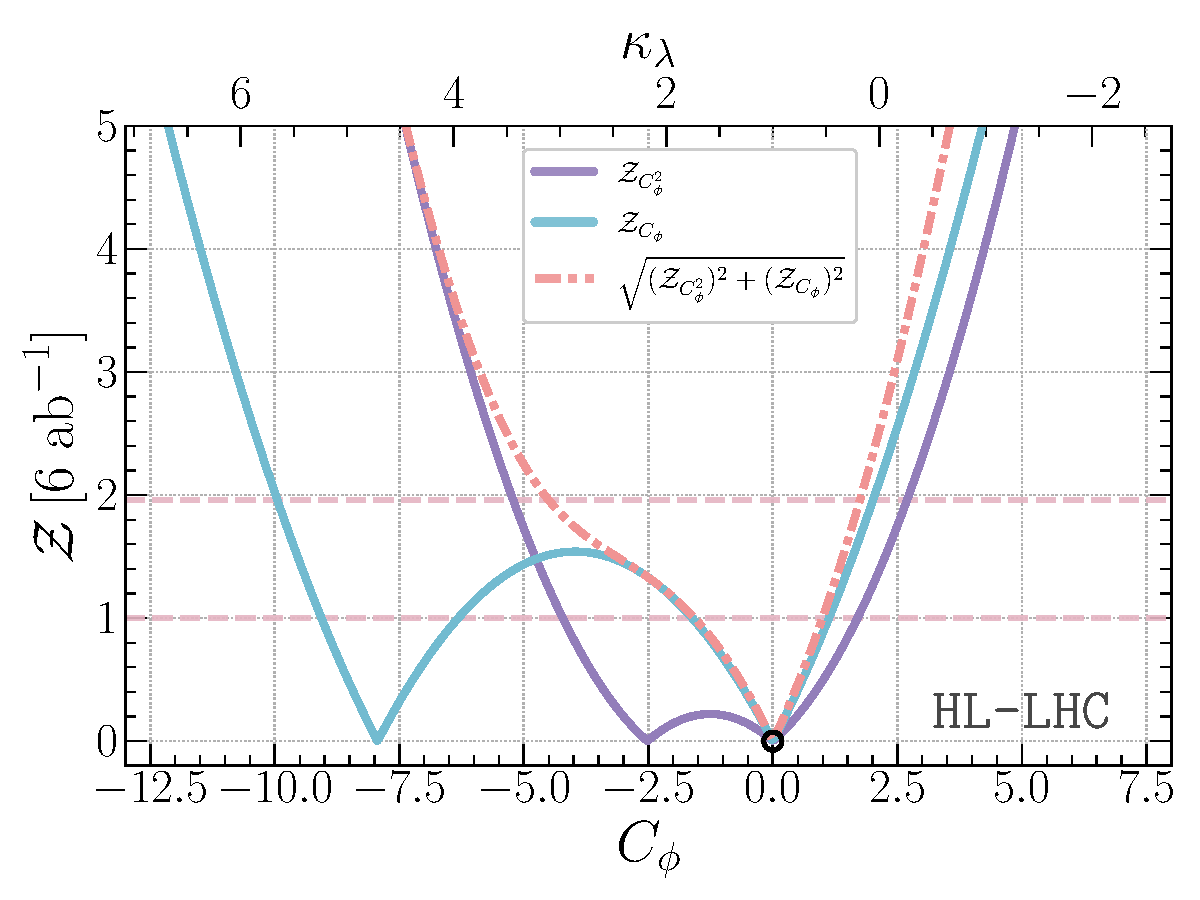
\includegraphics[width=0.55\linewidth]{fig/HL-LHC-sig14.pdf}
	%	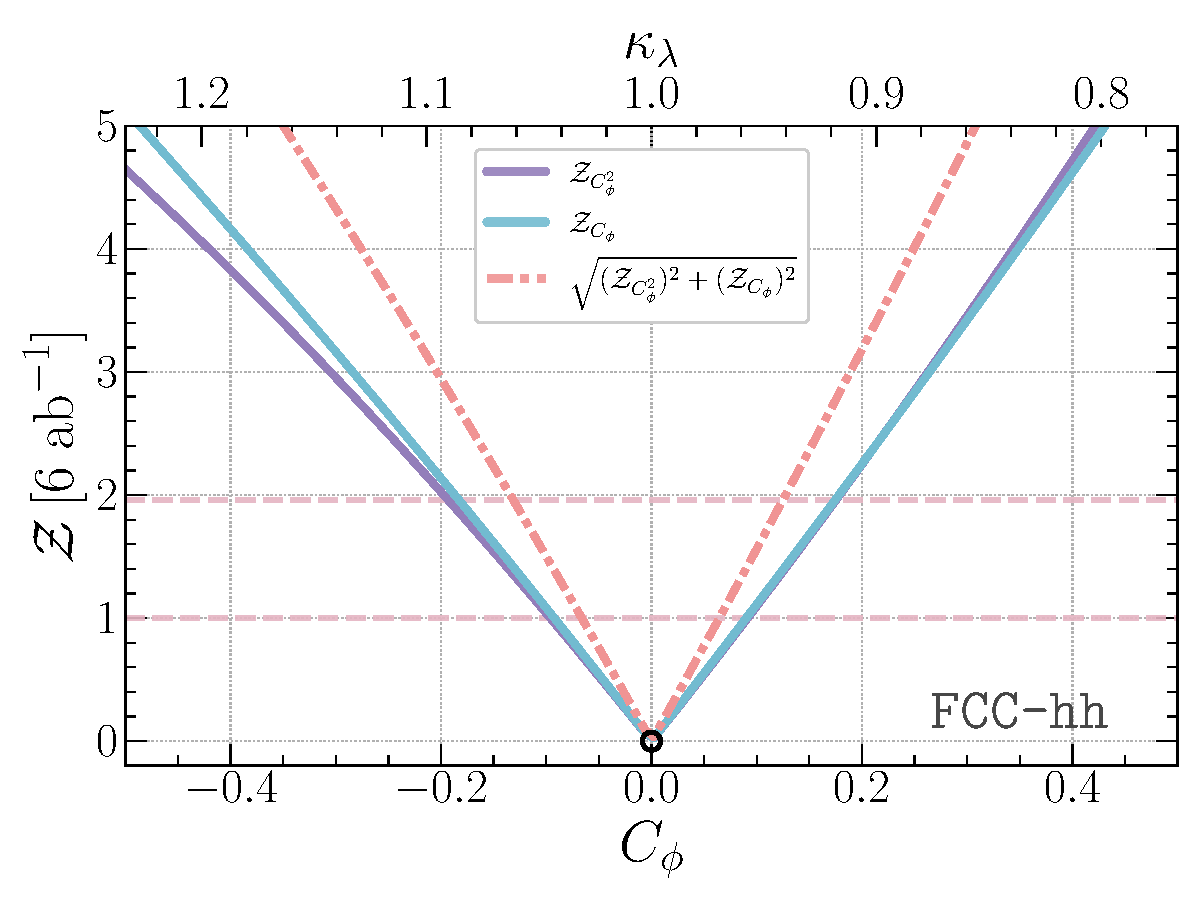
\includegraphics[width=0.47\linewidth]{fig/FCC-hh-sig100.pdf}
	\caption{ Bounds on $C_\phi$ (or $\kappa_\lambda$) at the HL-LHC from single parameter fit. The solid blue lines are the constraints from the $\hhint$ contribution, which scales linearly with the modified coupling. The solid purple line is from the $\hhtri$ contribution that scales quadratically with the modified coupling. The red dashed line is the combination of the quadratic and linear channels. The horizontal light red dashed lines mark the 68\% and 95\%CI's.}
	\label{fig:constraintkl}
\end{figure}
Another advantage of the optimised multivariate analysis is the ability to perform two-parameter fits in the same planes described above, shown in~\autoref{fig:constraint2d} while maintaining the improvement over the cut-based one. 
Since the BDT training achieved sufficient accuracy for the seven-channel classifier, including up and down $\qqA$, the different ggF topologies and the backgrounds. It was possible to resolve all of the signal channels strata and their parametric dependence on the three Wilson coefficients $C_{u\phi},\ C_{d \phi}$ and $C_\phi$. A three-parameter fit is possible without degeneracies, as seen in~\autoref{fig:constraint3d}.  However, the posterior distribution of the three-parameter fit shows no marked correlations amongst the Wilson coefficients. In both two- and three-parameter fits, a degeneracy in the $C_{d\phi}$ direction is observed at 99.7\$ CI. This is due to the reduction of the Higgs pair signal when the~$ h \to d \bar d$ decay channel is opened, particularly for high values of this Wilson coefficient as highlighted by~\autoref{signal_strength_hh}. When this analysis is applied for the strange quark, the overall effect of enhanced the strange quark is a reduction in the $ b \bar b \gamma \gamma$ signal, making this Higgs pair final state insensitive to the strange Yukawa enhancements; more details on this were discussed in ref.~\cite{Alasfar:2019pmn}. 
\begin{figure}[htpb!]
	\centering
	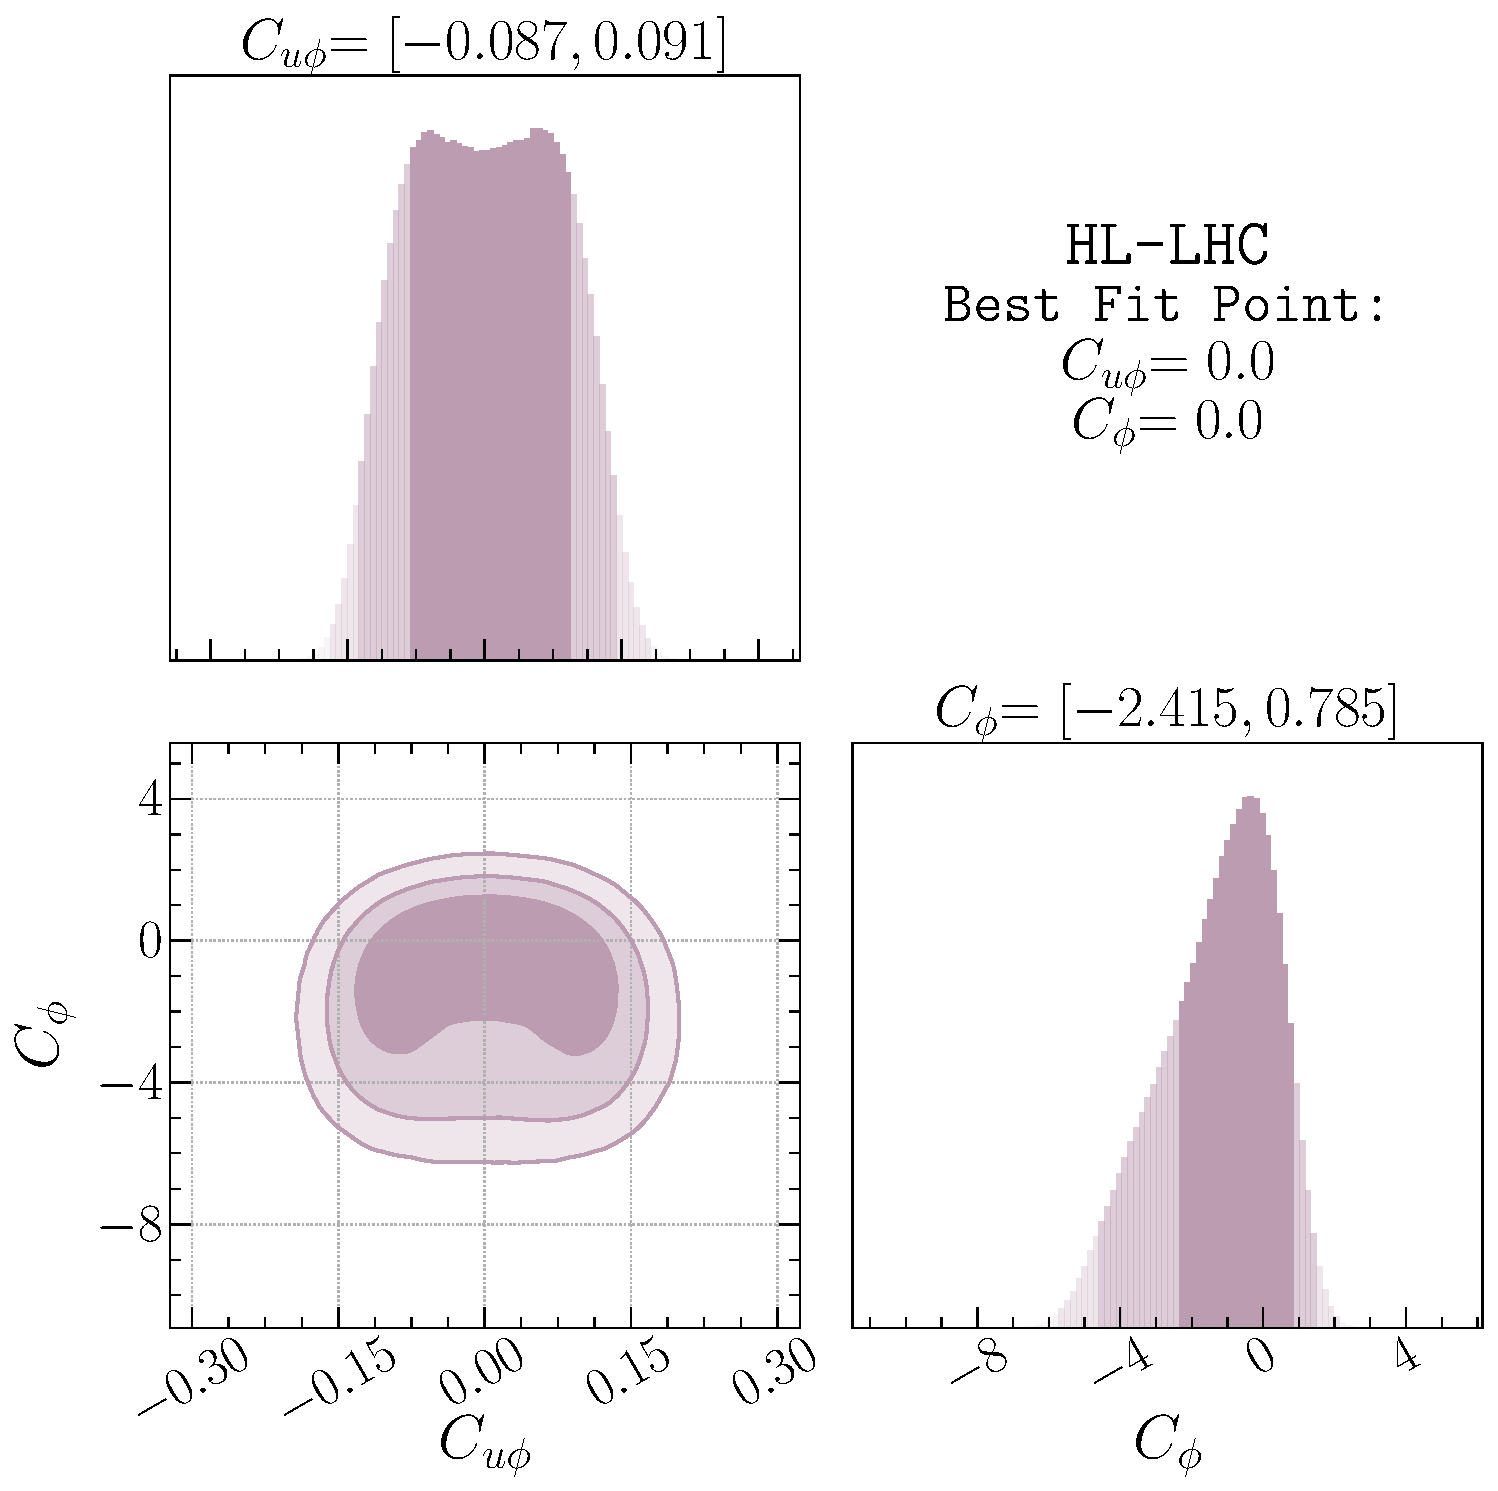
\includegraphics[width=0.4\linewidth]{fig/kappa_u-kappa_l-HL-LHC.pdf}
	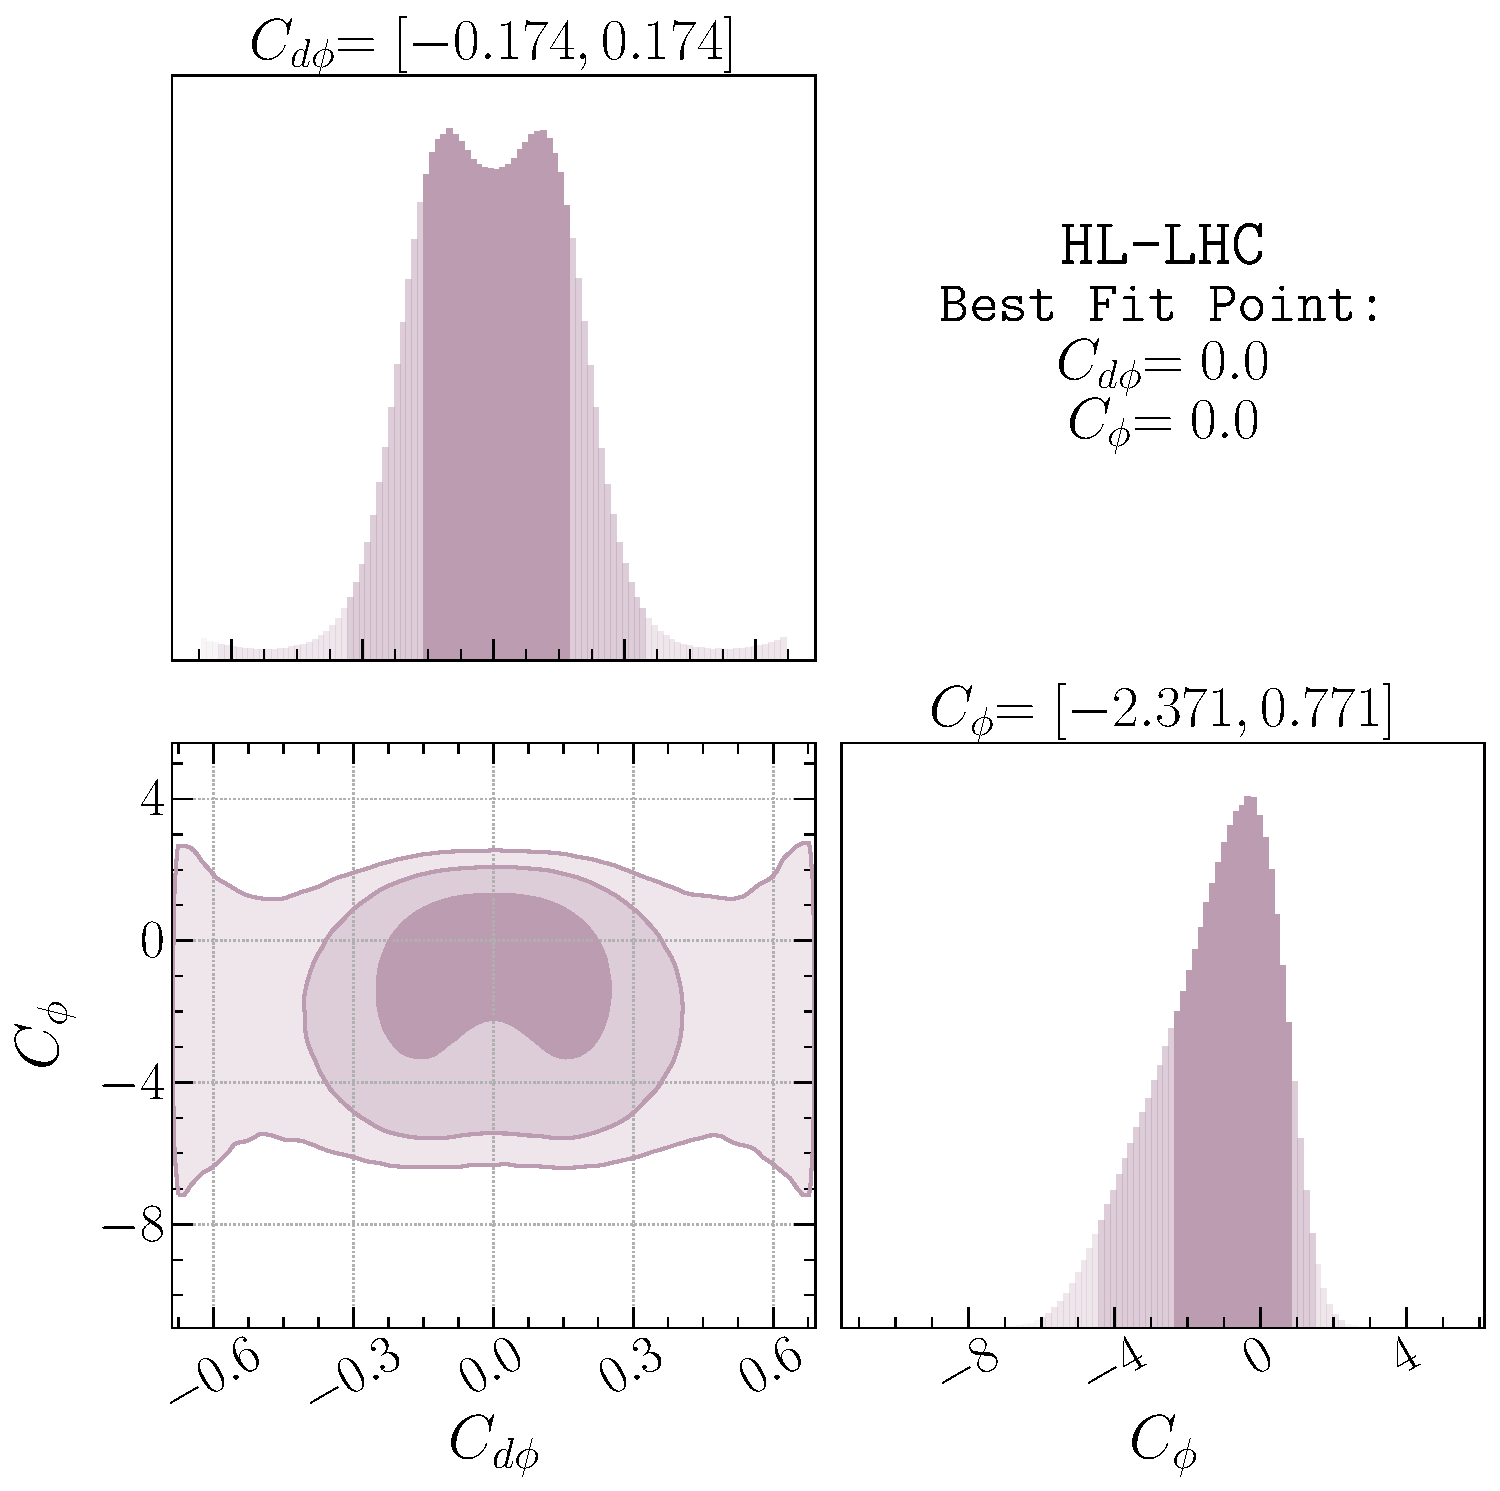
\includegraphics[width=0.4\linewidth]{fig/kappa_d-kappa_l-HL-LHC.pdf}
	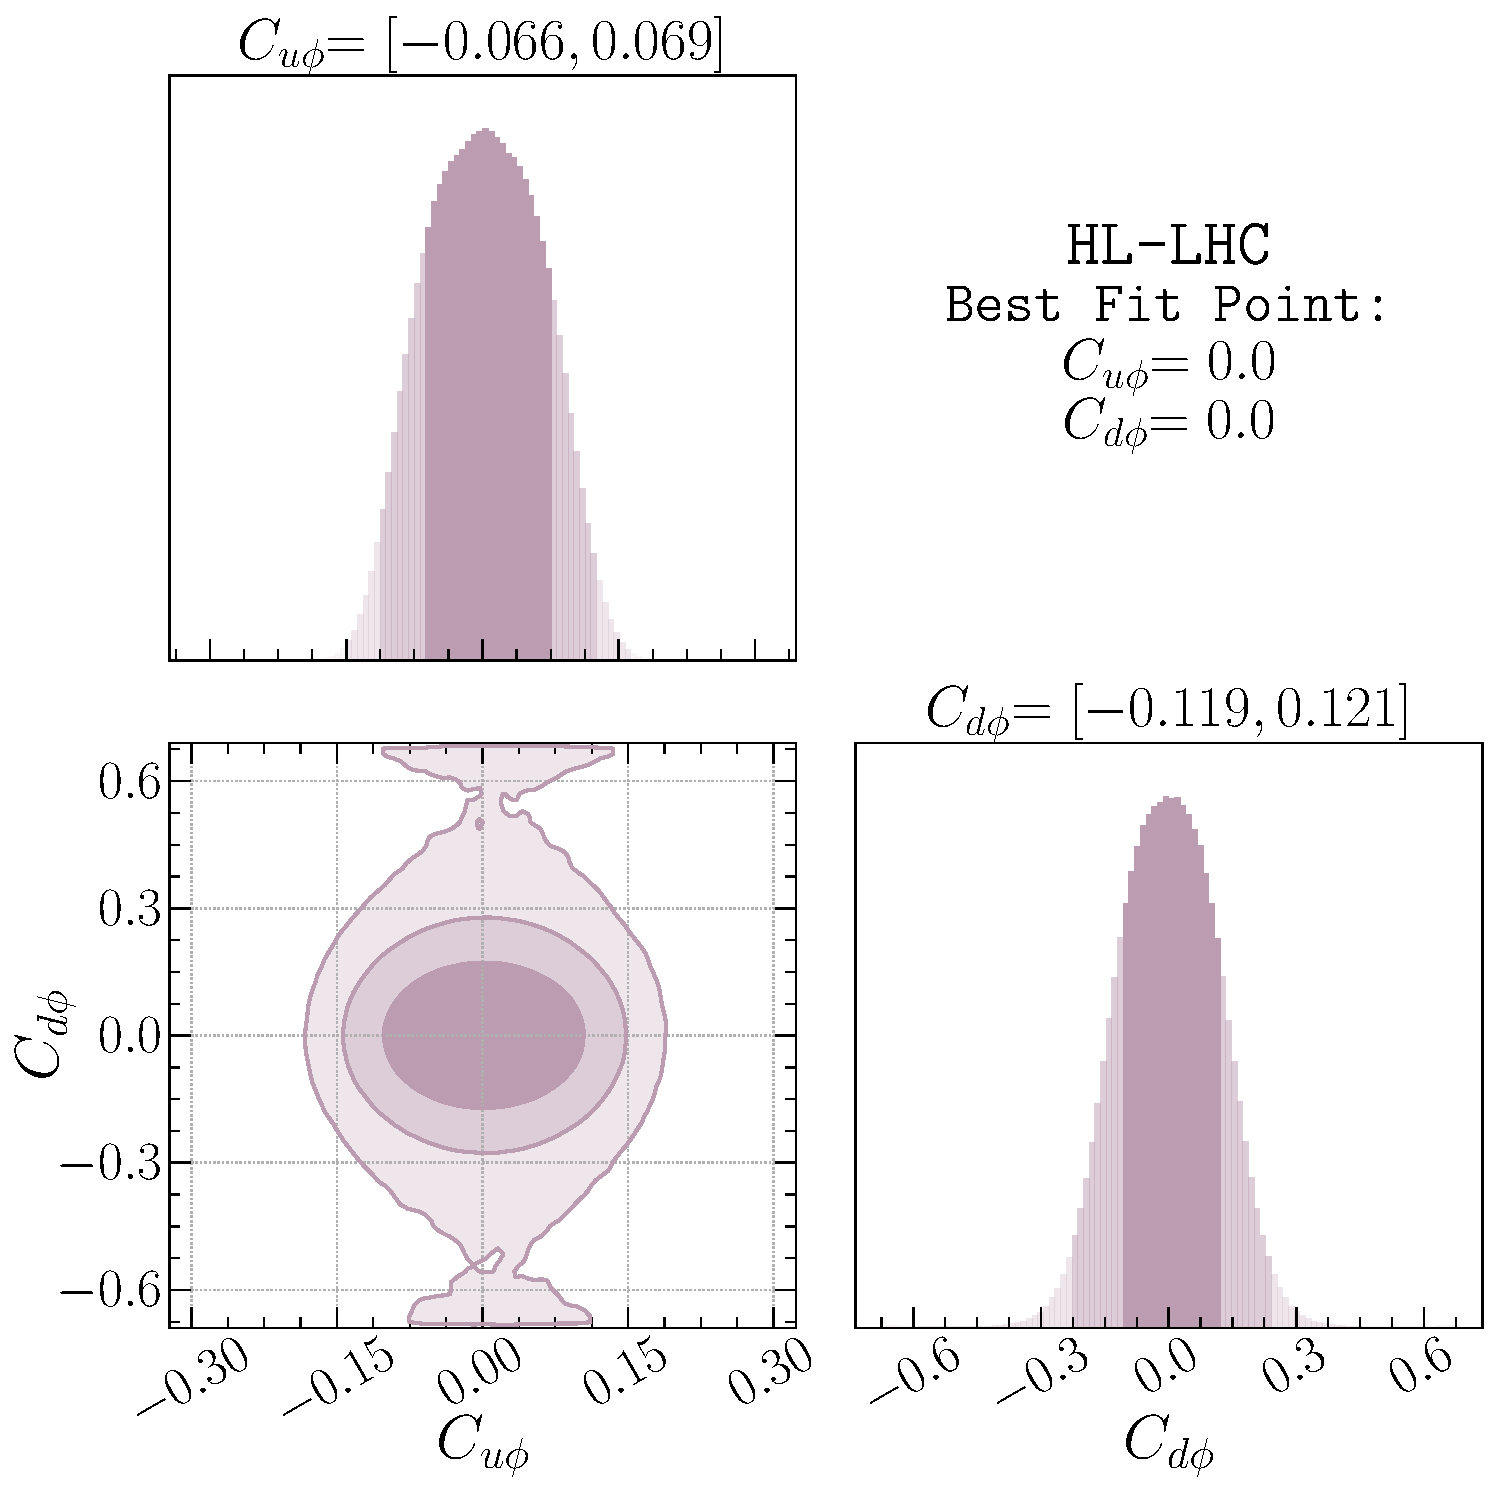
\includegraphics[width=0.4\linewidth]{fig/kappa_u-kappa_d-HL-LHC.pdf}
	\caption{The  68\%, 95\% and 99.7\% highest density posterior contours, for Bayesian fits preformed on pairs of Wilson coefficients for $C_\phi$, $C_{u\phi}$ and $C_{d\phi}$ form the multi-variate analysis output. The quoted intervals on top of the panel correspond to the 68\% CIs.}
	\label{fig:constraint2d}
\end{figure}
\begin{figure}[t!]
	\centering
	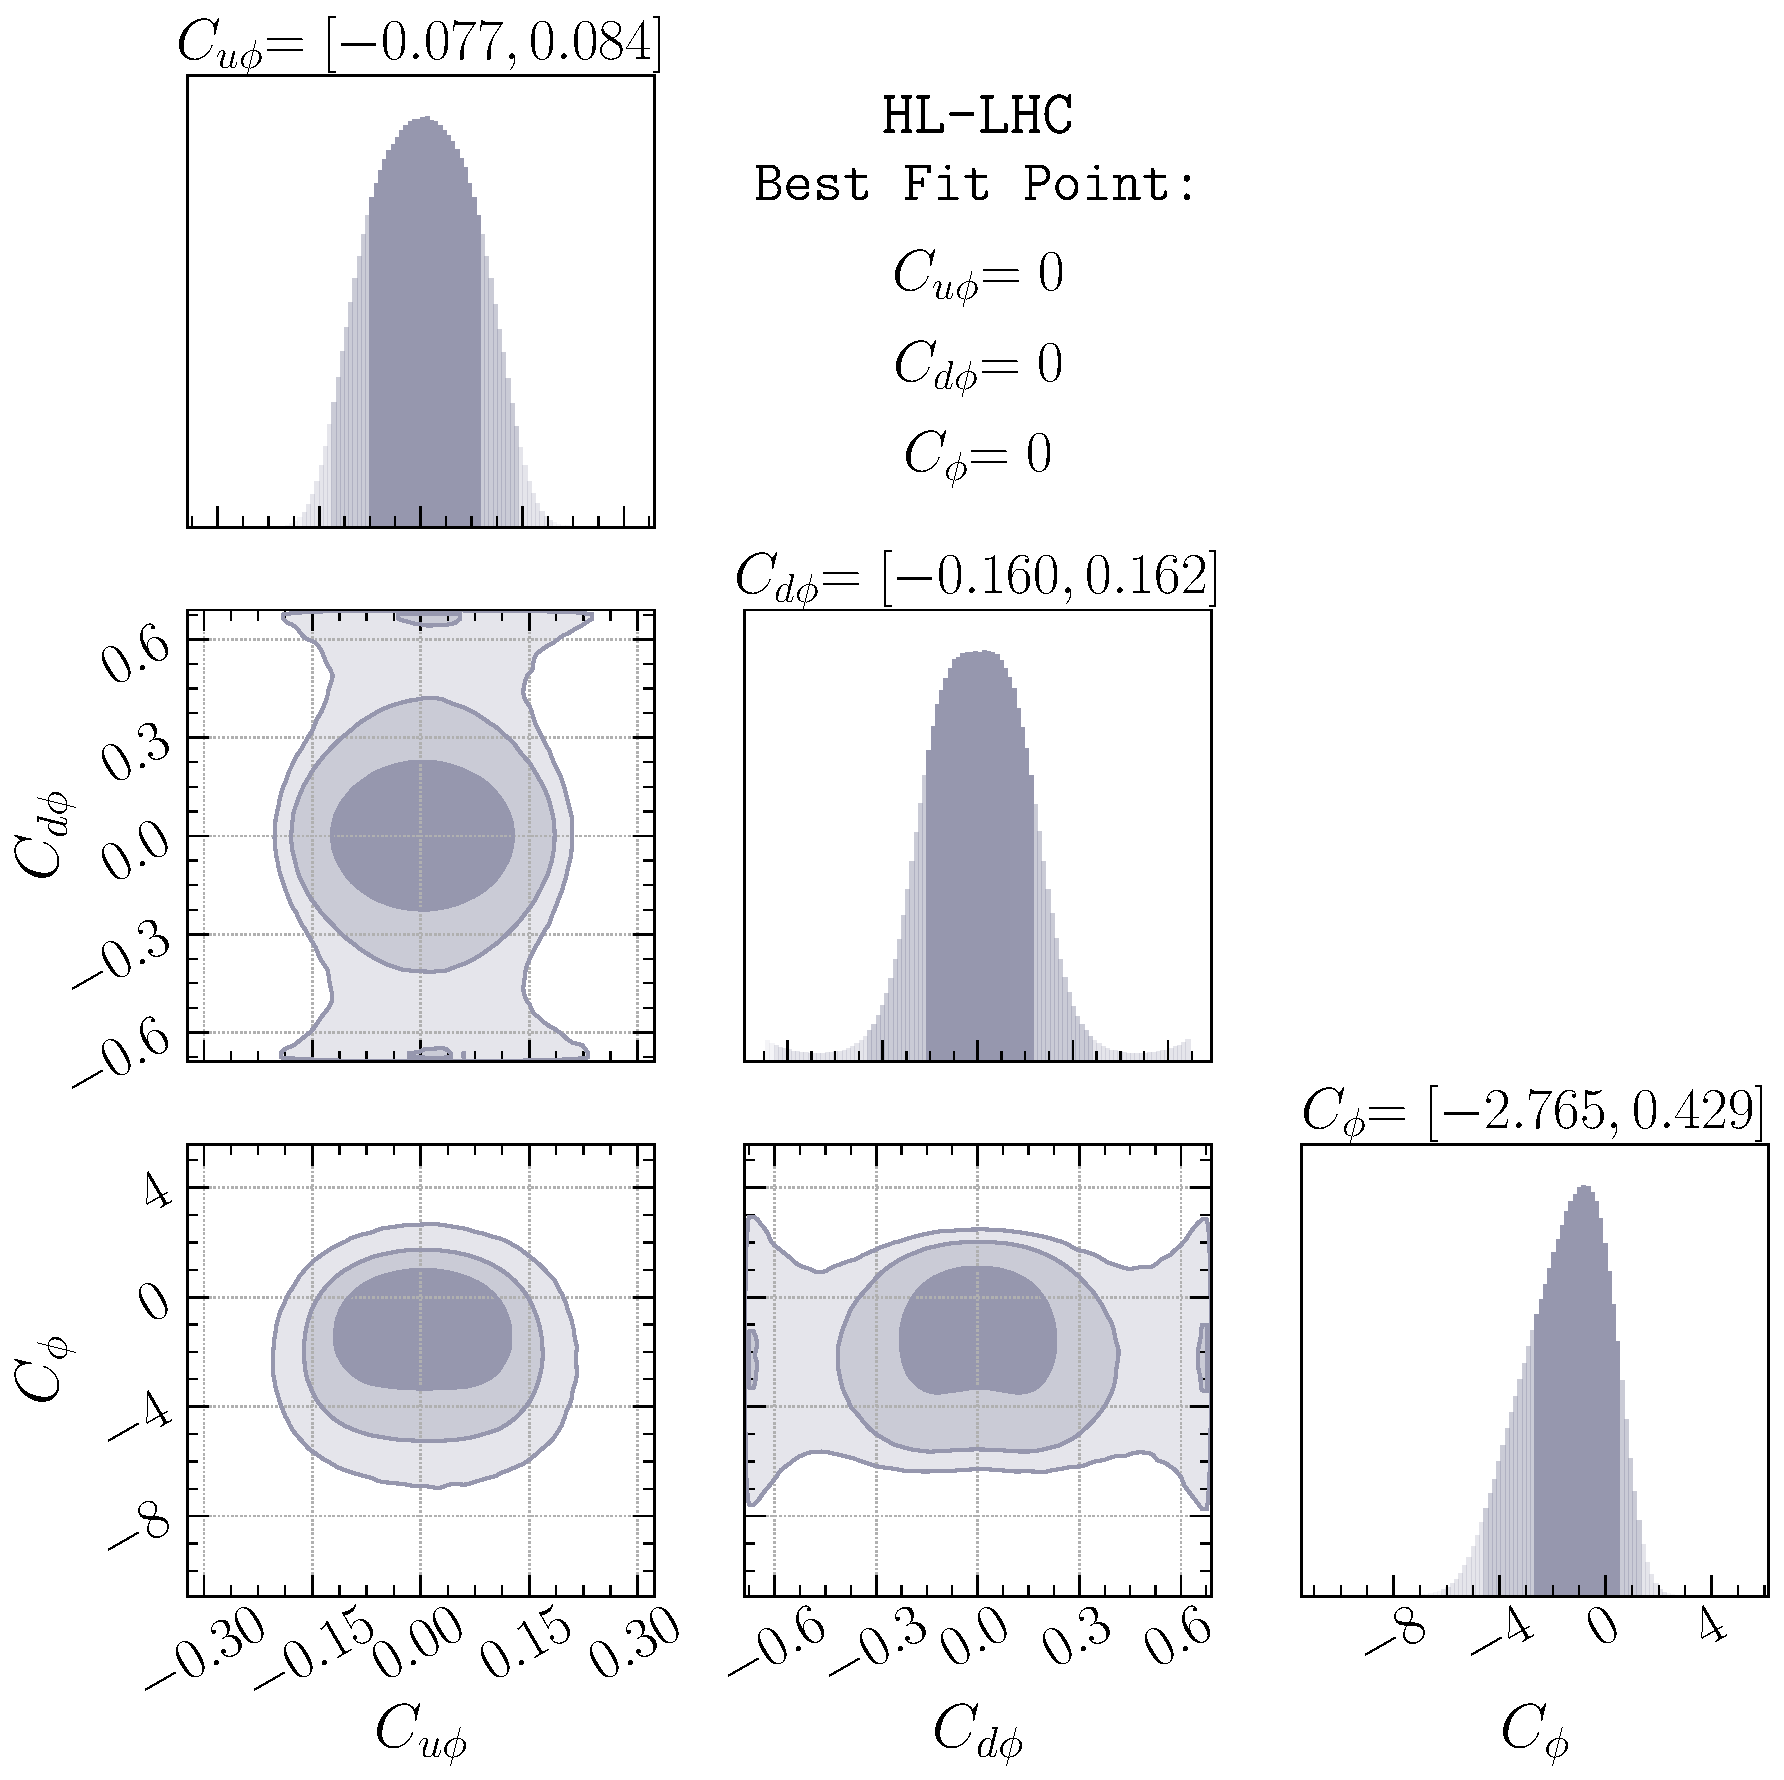
\includegraphics[width =0.65\linewidth]{fig/kappa_u-kappa_d-kappa_l-HL-LHC.pdf}
	\caption{ Three parameter Bayesian fits with $C_{u\phi}$, $C_{d\phi}$ and $C_\phi$, the highest density posterior contours are the same as~\autoref{fig:constraint2d}.}
	\label{fig:constraint3d}
\end{figure}
Comparing with the constraints on $C_\phi$ from a single parameter fit in~\autoref{fig:constraintkl}, it can be seen from the two- and three-parameter fits in~\autoref{fig:constraint2d} and~\autoref{fig:constraint3d}, respectively,  that, the constraints on $C_\phi$ become diluted when the light-quark Yukawa coupling modifiers $C_{q\phi}$ are taken into an account. This effect is somewhat more prominent for $C_{d\phi}$ than for $C_{u\phi}$ and stems from the fact that away from $C_{u\phi,d\phi} = 0$ larger negative values of $C_\phi$ are allowed by the crescent shaped curves of the highest density posterior contours. The bounds on $C_{u\phi}$ and $C_{d\phi}$ from the fit with two-parameters including $C_\phi$ remain the same as the bounds on these Wilson coefficient from the single parameter $C_{u\phi,d\phi}$ fits.  The fit results are summarised in~\autoref{tab:twoparambounds}. 
\begin{table}[]
	\centering
	{\footnotesize
		\begin{tabular}{cccc||ccc}
			\toprule
			Operators &  $C_{u\phi}$&   $C_{d\phi}$&   $C_{\phi}$&    $\kappa_{u}$&   $\kappa_{d}$&   $\kappa_\lambda$\\
			\midrule
			\multicolumn{7}{c}{HL-LHC 14 TeV 6$\inab$ @ 68\% CI}\\
			\midrule
			$\mathcal O_{\phi}$ &--   & --            &[-1.57, 1.00] &--  & -- &[0.53, 1.73]\\
			$\mathcal O_{u\phi}$&[-0.09, 0.10]   & --            &-- &[-477, 431]  & -- &--\\
			$\mathcal O_{d\phi}$&--   & [-0.16, 0.16]            &-- &--  & [-360, 360] &--\\
			$\mathcal O_{u\phi}$ \& $\mathcal O_{\phi}$ &[-0.087, 0.091]  & --            &[-2.42, 0.79] &[-434, 417] & -- &[0.63, 2.13]\\
			$\mathcal O_{d\phi}$ \& $\mathcal O_{\phi}$ & --             &[-0.17, 0.17]  &[-2.73, 0.77]& -- &[-381, 379] &[0.63, 2.27]\\
			$\mathcal O_{u\phi}$ \& $\mathcal O_{d\phi}$&[-0.065, 0.069]&[-0.12, 0.12]& --            &[-331, 312] &[-268, 272] & -- \\
			All                                   &[-0.077, 0.084]&[-0.160, 0.162]& [-2.77, 0.43]&[-400, 369] &[-362, 359] & [0.79, 2.30] \\
			\bottomrule
		\end{tabular}
	}
	\caption{Summary of the 68\% projected bounds on $C_{u\phi}$, $C_{d\phi}$ and $C_\phi$ from single-, two- and three-parameter fits for HL-LHC with 6$\inab$. The corresponding bounds on the rescaling of the effective couplings, $\kappa_u$, $\kappa_d$ and $\kappa_\lambda$ are presented on the right side of the table.}
	\label{tab:twoparambounds}
\end{table}
%%%%%%%%%%%%%%%%%%%%%%%%%%%%%%%%%%%%%%%%%%%%%%%%%%
\section{Overview of Light Yukawa searches \label{sec:comparetoothers}}
%%%%%%%%%%%%%%%%%%%%%%%%%%%%%%%%%%%%%%%%%%%%%%%%%%
Additional measurements of the light-quark Yukawa couplings might become relevant at HL-LHC or future hadron colliders like the FCC-hh, a careful study of which is beyond the scope of this thesis. Yet, I attempt to include a discussion here to provide a comparison with the study presented in this chapter and to put it into proper context or to serve as a proposal for further studies.
The channel $pp \to h +j $ has been proposed as a probe for charm Yukawa coupling~\cite{Brivio:2015fxa} with charm-tagged jet having a potential bound of $\kappa_c\sim 1$ for the HL-LHC, depending on the charm-tagging scheme. This process could be used for the first and second generations’ Yukawa couplings by looking at the shapes of the kinematic distributions, the most important one being  $\pt$~\cite{Soreq:2016rae,Bishara:2016jga, Bonner:2016sdg}. The expected HL-LHC 95\% CL bounds are $\kappa_c \in [-0.6,3.0]$, $|\kappa_u |\lesssim 170 $ and $|\kappa_d| \lesssim 990$. The use of the $h+j$ process along with other single Higgs processes have also been suggested as indirect probes for Higgs self coupling~\cite{McCullough:2013rea,Gorbahn:2016uoy,Bizon:2016wgr,Degrassi:2016wml,Maltoni:2017ims,Degrassi:2021uik}, due to the contribution of the trilinear coupling to NLO electroweak corrections to these processes. In addition, experimental fits have been carried out for the trilinear coupling from single Higgs observables~\cite{CMS:2018rig,ATLAS:2019pbo}. 

It seems that for the HL-LHC, an optimal bound for the trilinear coupling can be obtained by combining both  data from the single-Higgs process as well as Higgs pair production~\cite{DiVita:2017eyz}, with 68\% CL bound on $\kappa_\lambda \in[0.1,2.3]$, compared to the expected bound of $\kappa_\lambda \in [0.0,2.5] \cup [4.9,7.4]$ coming from using di-Higgs measurements alone. Moreover, single Higgs processes, namely $Zh$ and $ W^\pm h$ production, could also be useful in probing charm-Yukawa coupling utilising a mixture of $b$- and $c$-tagging schemes leveraging the mistagging probability of $c$-jets as $b$-jets in $b$-tagging working points, and vice-versa, to break the degeneracy in the signal strength~\cite{Perez:2015lra}. This technique could probe $\kappa_c \sim 1$ in the FCC-hh. Of course, for the charm-Yukawa coupling, the constraints are set to improve significantly, as there has been a recent direct observation of $h\to c \bar c$~\cite{ATLAS-CONF-2021-021}. Therefore, from here on, I will mainly concentrate on the process with more potential for constraining Yukawa couplings of the first generation quarks. 

Rare Higgs decays to mesons, $h \to M +V ,\, \, M = \Upsilon, J/\Psi, \phi\dots$, were suggested as a probe for light-quark Yukawa couplings~\cite{Bodwin:2013gca,Kagan:2014ila,Konig:2015qat}, and there have been experimental searches for these decays~\cite{ATLAS-CONF-2021-021,CMS:2018gcm} with bounds on the branching ratios, $\mathcal{B} (h \to X, \gamma, \,\,\, X =\Upsilon, J/\Psi,  ) \sim 10^{-4} - 10^{-6}$ at 95\% CL. It was shown in ref.~\cite{Yu:2017vul}, that the charge asymmetry of the process $pp \to h W^+$ vs $ pp \to h W^-$ can be used as a probe for light-quark Yukawa couplings and to break the degeneracy amongst quark flavours. Moreover, the rare process $ pp \to h \gamma$ is also a possible way to distinguish between enhancements of the up-and down-Yukawa couplings~\cite{Aguilar-Saavedra:2020rgo} where the authors have estimated the bounds on the up quark Yukawa coupling of $\kappa_u\sim 2000$ at the HL-LHC. Despite some processes appearing more sensitive than others, one should think of these processes as complementary. 
\begin{figure}[t!]
	%	\centering
	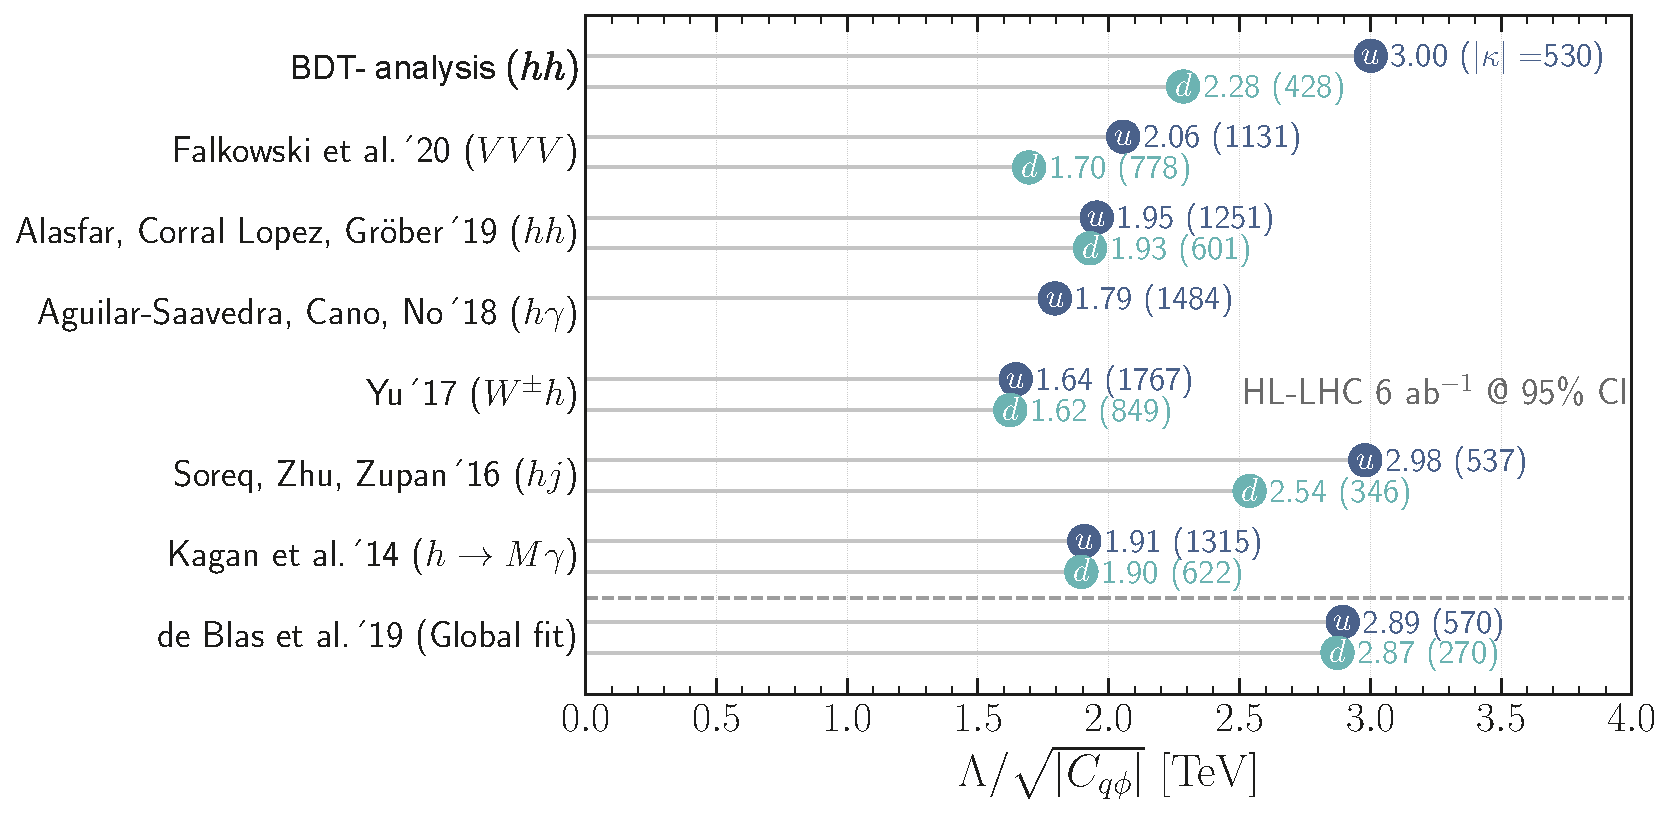
\includegraphics[width=\linewidth]{figures/ueberblick_ly.pdf}
	\caption{Summary of the $95\%$ CI/CL sensitivity bounds on the SMEFT Wilson coefficients $C_{u\phi}$ (blue), and $C_{d\phi}$ (green). The bounds are interpreted in terms of the NP scale $\Lambda$ that can be reached through the measurements of the Wilson coefficient at the HL-LHC at $6$ \invab, the corresponding $\kappa_q$'s are shown inside the parentheses. Single parameter fit $95\%$ CI bounds are used from this analysis for comparison with previous studies.}
	\label{fig:comparison}
\end{figure}
One of the main features of the effective couplings $hh q\bar q$ and $hhh q\bar q$ emerging from SMEFT operator $\mathcal O_{q\phi}$, or the EWChL for that matter, is that these couplings are either free from propagator suppression for $hh q\bar q$ or scale with energy for $hhh q\bar q$ while being safe from strong unitarity constraints. This feature gives processes with multiple Higgs and/or vector bosons $V= W^\pm, Z$ an advantage in constraining $\mathcal O_{q\phi}$. The latter constraints come from the longitudinal degrees of freedom of the gauge bosons, which can be understood from the Goldstone boson equivalence theorem. The use of the final state $VV$ as a probe for $\mathcal O_{q\phi}$ is difficult due to the large SM background. However, the three-boson final state $VVV$ gave strong projected bounds for light-quark Yukawa couplings for HL-LHC with 95\% CL bounds on $\kappa_u \sim 1600$and $\kappa_d\sim 1100$. A ten-fold improvement is expected at FCC-hh~\cite{Falkowski:2020znk} with bounds of order $\kappa_d\sim 30$. 
Higgs pair production has a smaller SM background compared to $VV$ production. Still, it has a significantly smaller cross-section, too, even when compared to $VVV$, as the latter process has already been observed at the LHC~\cite{Sciandra:2688061,CMS-PAS-SMP-19-014}.

On the contrary, Higgs pair production is inaccessible with the runs I-III of the LHC, but it is potentially accessible at the HL-LHC~\cite{Binoth:2006ym} having a $ \sigma \cdot BR\sim 1\mathrm{fb}^{-1}$. However, Higgs pair production, particularly the channel~$h \to b \bar b \gamma \gamma $, is of significant interest as it has unique features. The first is the ability to simultaneously constrain the trilinear and light-quark Yukawa couplings, as we have already seen in the previous sections. Secondly, Higgs pair production could probe non-linear relations between Yukawa interaction and~$hh q\bar q$ couplings~\cite{Contino:2012xk}. Lastly, Higgs pair production is expected to be significantly enhanced in specific models involving modification of light-quark Yukawa couplings (cf. ~\cite{Bar-Shalom:2018rjs,Bauer:2017cov,Egana-Ugrinovic:2021uew}).
A numerical comparison of the strongest bounds from HL-LHC on the first-generation Yukawa couplings from the studies discussed above in~\autoref{fig:comparison}. In contrast to the global fit bounds that have been obtained with no invisible or untagged Higgs decays allowed~\cite{deBlas:2019rxi}. For $C_{d\phi}$, the most stringent bound comes from the global fit and the $h+j$ channel as a model-independent bound, while this analysis provides the second most stringent model-independent bound. For $C_{u\phi}$, the BDT analysis presented here provided the most stringent constraint, while the bound from $h+j$ and the global analysis are comparable. The figure is interpreted in terms of the reach of NP scale $\Lambda$ that can be achieved by measuring these Wilson coefficients. For future colliders, like the FCC-hh at $100$ TeV, in addition to Higgs pair production, triple Higgs production might be an interesting channel for constraining the operators with Wilson coefficient $C_{u\phi}$ and $C_{d\phi}$ due to the energy increase of a Feynman diagram coupling the quarks to three Higgs bosons.\\
For future colliders, like the FCC-hh at $100$ TeV, in addition to Higgs pair production, triple Higgs production might be an interesting channel for constraining the operators with Wilson coefficient $C_{u\phi}$ and $C_{d\phi}$ due to the energy increase of a Feynman diagram coupling the quarks to three Higgs bosons.   In this case, a similar study to this one should be performed to investigate this potential further, also, in this case, it will be essential to do a combined fit on the light quark Yukawa couplings together with the trilinear and quartic Higgs self-couplings.\footnote{In~\cite{Papaefstathiou:2047255}, it was shown that $\sim \mathcal{O}(1)$ bounds on the quartic Higgs self-coupling can be reached at the FCC-hh.}
Finally, it should be noted that there are also non-collider signatures for enhanced light-quark Yukawa couplings, manifesting in frequency shifts in atomic clocks from Higgs forces at the atomic level~\cite{Delaunay:2016brc}. 
%%%%%%%%%%%%%%%%%%%%%%%%%%%%%%%
\section{Discussion and conclusion \label{sec:concly}}
%%%%%%%%%%%%%%%%%%%%%%%%%%%%%%%
The chapter walked through the potential of Higgs pair production to glean information about the elusive Yukawa couplings of the first generation quarks from the final state~$b\bar{b}\gamma \gamma$. This has been done in two different approaches: The first is the traditional cut and count method. Later on, I have showcased a significant improvement in the analysis by using interpretable machine learning.   To maintain harmony with other chapters of this thesis, the enhancements of light Yukawa couplings were parametrised within the SMEFT framework. \\ 
Despite the limitations of the cut-based analysis for the Higgs pair, it was still possible to estimate notable sensitivity for both up-and down-type Yukawa coupling to the Higgs boson, comparable with other channels and the model-dependent global fit.  Superior estimated bounds, particularly for the up quark, emanated from fully exploiting the kinematical shapes and their correlations in a multivariate analysis. This was achieved by using a high-level kinematical distribution as a feature in a BDT classification. The ML is interfaced with an explainer layer based on Shapley's values. \\ The precedence of using an interpretable ML framework over DNNs stems from optimising the training procedure by employing physics-motivated dimensionality reduction by excluding less important features.  Interpretable ML not only outperforms black-box models but also provides a physics understanding of the processes at hand, pointing to kinematic variables like $H_T$ and $m_{\gamma\gamma}$ as being important variables that instrument this separation. Lastly, but most importantly,  interpretable models provide higher confidence in the results of their classification or regression.\\
%%%%
The use of a BDT classifier was not only beneficial for increasing the $hh$ signal selection efficiency but also to classify the signal channels strata, such that it is possible to parametrise it in terms of $C_{\phi}$, $C_{u\phi}$ and $C_{d \phi}$, by decomposing the ggF channel into its sub-topologies depending on their $C_\phi$ parametrisation.   The outcome of this technique is the ability to perform two and three-parameter fits, including all of the Wilson coefficients in question. \\
%%
With the HL-LHC Higgs pair searches, it is expected to constrain the Higgs trilinear coupling to ~ $\mathcal{O}(1)$ of the SM prediction. A result matched by other sensitivity analyses based on ML analysis done by experimentalists at the CMS and ATLAS~\cite{ATL-PHYS-PUB-2018-053,ATLAS:2018rvj,CMS-PAS-FTR-18-011}. This highlights the desideratum of Higgs pair production observation for understanding the Higgs potential. Despite light Yukawa modifiers like $C_{q\phi}$ being typically overlooked when studying Higgs pair production, this study showed that they could dilute the bounds on the trilinear Higgs coupling. Thus these coefficients need to be considered in any phenomenological studies of the Higgs pair. These Wilson coefficients are weakly bounded from other measurements, unlike other coefficients constrained from single-Higgs, EWPO or top quark data. \\
%%
There exist a handful of potential UV-complete models in which both light Yukawa as well as the Higgs trilinear couplings are enhanced. For example, a model proposed in ref~\cite{Bar-Shalom:2018rjs} based on vector-like quarks~(VLQ) with AFV assumptions. The original assumption of this model is excluded, as the authors assumed an enhancement of all light quark-Higgs couplings to be equal to the beauty quark Yukawa. One could still get significant enhancement to light Yukawa from VLQ masses of $ \sim 2$ TeV, which is well above the current direct searches excluding VLQ of masses~$ M_{VLQ} < 1.6$ TeV ~\cite{Unal:2777832,CMS:2019eqb} for the hadronic final state, and $M_{VLQ}< 1.2$ TeV for the leptonic one~\cite{CMS:2018wpl}. Due to the AFV manifested in this model, the VLQ could be made not to couple to the third generation quarks and evade the tree-level EWPO bounds ~\cite{Dawson:2020oco}. In addition, the trilinear Higgs coupling could be modified by the inclusion of an additional scalar singlet cf.~\cite{DiLuzio:2017tfn, Falkowski:2019tft, Chang:2019vez}.  Another example of models with enhanced light Yukawa is a two-Higgs-doublet model (2HDM) model proposed in refs.~\cite{Egana-Ugrinovic:2019dqu,Egana-Ugrinovic:2021uew}. This model has a special kind of AFV, known as spontaneous flavour violation~(SFV).  Enhancements to light Yukawa couplings come from the second Higgs Yukawa couplings, which are made diagonal in the flavour space ~$K_{q}$ ($q=u,d$). SFV has the constraint that either the up-type or the down-type couplings can be enhanced, while the couplings of the other type maintain the SM hierarchy. 
\begin{figure}[!t]
	\centering
	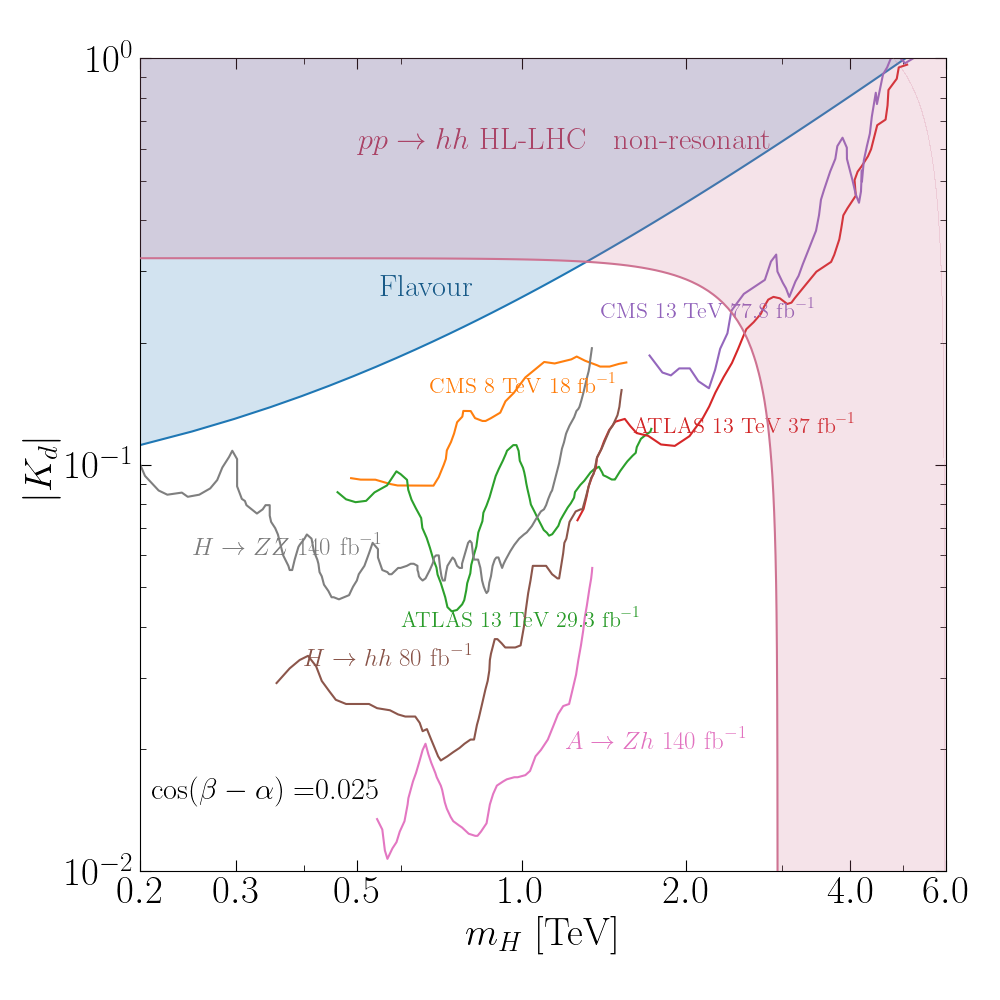
\includegraphics[width = 0.5\textwidth]{./fig/2HDM-bound_full}
	\vspace{-0.5 cm}
	\caption{Example of constraints on the 2HDM with SFV presented in~\cite{Egana-Ugrinovic:2019dqu,Egana-Ugrinovic:2021uew} from flavour observables, LHC dijet , $Zh$,$ZZ$ and resonant $hh$ searches. The region shaded in Red is the bounds projected for the HL-LHC from the analysis presented in this chapter. This plot is based on the results quoted in ref.~\cite{Egana-Ugrinovic:2021uew}. } % verify the notation
	\label{fig_uv_qqhh}
\end{figure}
The addition of the second doublet modifies the Higgs potential, and consequently, the Higgs self-coupling will be modified as well.  Like any other 2HDM, the parameter space is rather large. The bounds on this model will depend on the region of its parameter space we are interested in.  ~\autoref{fig_uv_qqhh} shows the bounds on this model for a point near the alignment limit. For a small mass of the ``heavy'' Higgs $H$ and large Yukawa coupling~$K_d$ flavour bounds dominate, while for larger $m_H$, the dijet searches~\cite{Aaboud:2019zxd,Aad:2019hjw,Sirunyan:2019vgj}  would dominate due to the decay $ H \to d \bar d$.  On the contrary, the decay $ H \to hh$ would become dominant from smaller values of $K_d$ and larger $H$ mass, but still $ m_H < 2$ TeV. In this regime, resonant Higgs pair searches give string constraints for light Yukawa enhancement~\cite{Sirunyan:2018ayu, Aad:2019uzh}. Similar  light Yukawa bounds in this region of the parameter space could also be derived from  $Zh$~\cite{ATLAS:2020pgp} and $ZZ$~\cite{Aad:2020fpj, Sirunyan:2018qlb} searches.  Lastly, for $ m_H > 2$ TeV, the non-resonant Higgs pair production will become the dominant bound on light Yukawa enhancement, coming from the analysis of this chapter.  


